\documentclass[a4paper,11pt,twoside,openright,bibtotoc,liststotoc,tablecaptionabove]{fsd}
\renewcommand*{\familydefault}{\sfdefault}
\usepackage{helvet}
\newcommand{\mytitle}{Rigid Track Position Tracking}
\newcommand{\myauthor}{Florian Wachter}
\newcommand{\pagez}{73}
\usepackage[utf8]{inputenc}
\usepackage{amsmath}
\usepackage{amssymb}
\usepackage{amsfonts}
\usepackage{amssymb}
\usepackage{ltxtable} 
\usepackage{longtable}
\usepackage[table]{xcolor}
\usepackage{graphicx}
\usepackage[absolute, overlay]{textpos}
 \setlength{\TPHorizModule}{1mm}
 \setlength{\TPVertModule}{1mm}
\usepackage{acronym}
\usepackage[pdfpagelayout=TwoPageRight, breaklinks]{hyperref}
\usepackage[hyphenbreaks]{breakurl}
\usepackage{eurosym}
\usepackage{float}
\usepackage{blindtext}
\usepackage{paralist}
\usepackage{tabto}
\usepackage{placeins}
\usepackage[toc,page]{appendix}
\usepackage{listings}
\usepackage{booktabs}
\usepackage{rotating}
\usepackage{multirow}
\usepackage{setspace}
\usepackage{wrapfig}
\usepackage{svg}
\usepackage{wasysym}
\usepackage{import}
\usepackage{epstopdf}
\usepackage{footnote}
\usepackage{scrextend}
\usepackage{eso-pic}
\usepackage{siunitx}
\usepackage{forest}
\usepackage{pdfpages}

% Hurenkinder und Schusterjungen verhindern
\clubpenalty = 10000
\widowpenalty = 10000
\displaywidowpenalty = 10000

\setlength{\parindent}{0pt}

\usepackage{nicefrac}
\setlength{\parskip}{0.em}

\newcommand{\sh}{{}}
		
\usepackage[autostyle,english=american]{csquotes}


\def\Size{4pt}

	
\newcommand{\tabitem}{~~\llap{\textbullet}~~}


\newcommand{\ANSISafety}[2]{
	\vbox{%
	\paragraph{}
	\begin{addmargin}[7em]{0.1em}
	\hspace{-7em}
	\IfEqCase{#1}{
	{Warning}{
		\includegraphics[height = 1.2em]{Grafiken/warning.pdf}\hspace{1em}{#2}
	}
	{Danger}{
		\includegraphics[height = 1.2em]{Grafiken/danger.pdf}\hspace{1em}{#2}
	}
	{Caution}{
		\includegraphics[height = 1.2em]{Grafiken/caution.pdf}\hspace{1em}{#2}
	}
	{Notice}{
		\includegraphics[height = 1.2em]{Grafiken/notice.pdf}\hspace{1em}{#2}
	}
	}
	\end{addmargin}
	\vspace{1em}
}
}


\bibliography{MA.bib}

\usepackage{etoolbox}
\makeatletter
\makeatother



\newcommand*{\fullref}[1]{\hyperref[{#1}]{\autoref*{#1} (\nameref*{#1})}} % One single link

% Packages required by doxygen
\usepackage{fixltx2e}
\usepackage{calc}
\usepackage{doxygen}
\usepackage[export]{adjustbox} % also loads graphicx
\usepackage{graphicx}
\usepackage[utf8]{inputenc}
\usepackage{makeidx}
\usepackage{multicol}
\usepackage{multirow}
\PassOptionsToPackage{warn}{textcomp}
\usepackage{textcomp}
\usepackage{sectsty}

\newcommand{\+}{\discretionary{\mbox{\scriptsize$\hookleftarrow$}}{}{}}


\renewcommand{\sectionmark}[1]{%
	\markright{\thesection\ #1}%
}


% Hyperlinks (required, but should be loaded last)
\usepackage{ifpdf}
\hypersetup{%
	colorlinks=true,%
	linkcolor=blue,%
	citecolor=blue,%
	unicode%
}

% Custom commands
\newcommand{\clearemptydoublepage}{%
	\newpage{\pagestyle{empty}\cleardoublepage}%
}

\usepackage{caption}
\captionsetup{labelsep=space,justification=centering,font={bf},singlelinecheck=off,skip=4pt,position=top}



\begin{document}
%	\AddToShipoutPicture{\BackgroundPic} 



\thispagestyle{empty}
\begin{textblock}{70}(25,26)
	\centering
	\fontsize{14}{18}
	\hspace{1.3cm}\scalebox{1.12}[1]{Technische Universität München}\\
	\vspace{0.488cm}\hspace{0.97cm}
	\includegraphics[height=1.82cm]{Grafiken/TUMLogo_oZ_Vollfl_blau_CMYK}
\end{textblock}
\begin{textblock}{80}(105,26)
	\centering
	\fontsize{14}{18}
	\hspace{0.2cm}\scalebox{1.12}[1]{Institute for Flight System Dynamics}\\
	\vspace{0.41cm}\hspace{-0.1cm}
	\includegraphics[height=1.83cm]{grafiken/fsd_logo}
\end{textblock}


\begin{center}
	\hspace*{1.5cm}
\begin{minipage}{0.7\linewidth}
    \centering
    \vspace{5.45cm}
%Thesis title
    {\uppercase {\Huge \mytitle\par}}
    \vspace{0.635cm}
    \rule{0.035\textwidth}{2pt}
    \vspace{0.8cm}\\
   Doxygen Generated Documentation\\
    \vspace{1cm}
    \Huge \scalebox{0.9}[0.95]{Documentation}
    \vspace{4.7cm}
    
	\large 

	Author: Florian Wachter\\
	\vspace{0.32cm}
	Matriculation Number: 3628475
	
	
\end{minipage}
\end{center}
\clearpage

\newpage
\thispagestyle{fancy}
\fancyhf{}

\mbox{}


\setcounter{page}{1}
\tableofcontents

\pagestyle{plain}

\mbox{}



%--- Begin generated contents ---
\chapter{Rigid Track Doxygen Documentation}
\label{index}\hypertarget{index}{}\hypertarget{index_intro_sec}{}\section{Introduction}\label{index_intro_sec}
Rigid Track is a software that provides, combined with an Opti\+Track camera, the pose estimation of one object in three dimensional space. This is achieved with only one camera in combination with reflective markers. Those are attached to the object ought to be tracked. The accuracy in the range of millimeters and the high update rate of 100 Hz enable use cases for fast and agile objects. The main application is navigation for drones that rely on high precision position data. Where G\+PS is not available, e.\+g. indoors or due to a lacking G\+PS receiver, this setup substitutes for it. Another use case is the pure pose logging when the drone does not depend on the position, e.\+g. when it is remote piloted by hand. While this setup contains one Opti\+Track Flex 3 camera, every other model of Opti\+Track should work, despite not tested. With better camera models, e.\+g. the Prime Series, even outdoor usage is possible. When the capabilities are not sufficient please refer to Opti\+Tracks Software Motive. But keep in mind that this solution needs at least 3 cameras as Rigid Track works with only one.\hypertarget{index_softInstall_sec}{}\section{Rigid Track Installation}\label{index_softInstall_sec}
Start the Rigid\+Track\+\_\+setup.\+exe from the enclosed SD card and follow the instructions given in the installation assistant. Default parameters like installation directory or shortcuts to be created can be chosen. But normally clicking Next and keeping the default values should be sufficient. When the installation is completed a shortcut in the start menu and the desktop can be used to start Rigid Track. The program is then successfully installed in C\+:/\+Program Files (x86)/\+TU Munich F\+S\+D/\+Rigid Track.\hypertarget{index_source_code}{}\section{Source Code}\label{index_source_code}
The most interesting file for you is \hyperlink{main_8cpp}{main.\+cpp}. It contains the relevant functions for pose estimation. Camera calibration and other functional aspects are also implemented there. The G\+UI program code is found in \hyperlink{_rigid_track_8cpp}{Rigid\+Track.\+cpp}. \hyperlink{communication_8cpp_source}{communication.\+cpp} deals only with communication from \hyperlink{main_8cpp}{main.\+cpp} to the G\+UI. 
\chapter{File Index}
\section{File List}
Here is a list of all files with brief descriptions\+:\begin{DoxyCompactList}
\item\contentsline{section}{Rigid\+Track/\hyperlink{__modelest_8h}{\+\_\+modelest.\+h} }{\pageref{__modelest_8h}}{}
\item\contentsline{section}{Rigid\+Track/\hyperlink{communication_8cpp}{communication.\+cpp} }{\pageref{communication_8cpp}}{}
\item\contentsline{section}{Rigid\+Track/\hyperlink{communication_8h}{communication.\+h} }{\pageref{communication_8h}}{}
\item\contentsline{section}{Rigid\+Track/\hyperlink{_import_log_8m}{Import\+Log.\+m} }{\pageref{_import_log_8m}}{}
\item\contentsline{section}{Rigid\+Track/\hyperlink{main_8cpp}{main.\+cpp} }{\pageref{main_8cpp}}{}
\item\contentsline{section}{Rigid\+Track/\hyperlink{main_8h}{main.\+h} }{\pageref{main_8h}}{}
\item\contentsline{section}{Rigid\+Track/\hyperlink{precomp_8hpp}{precomp.\+hpp} }{\pageref{precomp_8hpp}}{}
\item\contentsline{section}{Rigid\+Track/\hyperlink{resource_8h}{resource.\+h} }{\pageref{resource_8h}}{}
\item\contentsline{section}{Rigid\+Track/\hyperlink{_rigid_track_8cpp}{Rigid\+Track.\+cpp} }{\pageref{_rigid_track_8cpp}}{}
\item\contentsline{section}{Rigid\+Track/\hyperlink{_rigid_track_8h}{Rigid\+Track.\+h} }{\pageref{_rigid_track_8h}}{}
\item\contentsline{section}{Rigid\+Track/\hyperlink{simpleplot_8m}{simpleplot.\+m} }{\pageref{simpleplot_8m}}{}
\item\contentsline{section}{Rigid\+Track/\hyperlink{supportcode_8cpp}{supportcode.\+cpp} }{\pageref{supportcode_8cpp}}{}
\item\contentsline{section}{Rigid\+Track/\hyperlink{supportcode_8h}{supportcode.\+h} }{\pageref{supportcode_8h}}{}
\item\contentsline{section}{Rigid\+Track/\+Generated\+Files/\hyperlink{qrc___rigid_track_8cpp}{qrc\+\_\+\+Rigid\+Track.\+cpp} }{\pageref{qrc___rigid_track_8cpp}}{}
\item\contentsline{section}{Rigid\+Track/\+Generated\+Files/\hyperlink{ui___rigid_track_8h}{ui\+\_\+\+Rigid\+Track.\+h} }{\pageref{ui___rigid_track_8h}}{}
\item\contentsline{section}{Rigid\+Track/\+Generated\+Files/\+Debug/\hyperlink{_debug_2moc__communication_8cpp}{moc\+\_\+communication.\+cpp} }{\pageref{_debug_2moc__communication_8cpp}}{}
\item\contentsline{section}{Rigid\+Track/\+Generated\+Files/\+Debug/\hyperlink{_debug_2moc___rigid_track_8cpp}{moc\+\_\+\+Rigid\+Track.\+cpp} }{\pageref{_debug_2moc___rigid_track_8cpp}}{}
\item\contentsline{section}{Rigid\+Track/\+Generated\+Files/\+Release/\hyperlink{_release_2moc__communication_8cpp}{moc\+\_\+communication.\+cpp} }{\pageref{_release_2moc__communication_8cpp}}{}
\item\contentsline{section}{Rigid\+Track/\+Generated\+Files/\+Release/\hyperlink{_release_2moc___rigid_track_8cpp}{moc\+\_\+\+Rigid\+Track.\+cpp} }{\pageref{_release_2moc___rigid_track_8cpp}}{}
\end{DoxyCompactList}

\chapter{File Documentation}
\hypertarget{main_8cpp}{}\section{Rigid\+Track/main.cpp File Reference}
\label{main_8cpp}\index{Rigid\+Track/main.\+cpp@{Rigid\+Track/main.\+cpp}}
{\ttfamily \#include \char`\"{}Rigid\+Track.\+h\char`\"{}}\newline
{\ttfamily \#include \char`\"{}main.\+h\char`\"{}}\newline
{\ttfamily \#include \char`\"{}communication.\+h\char`\"{}}\newline
{\ttfamily \#include \char`\"{}cameralibrary.\+h\char`\"{}}\newline
{\ttfamily \#include \char`\"{}modulevector.\+h\char`\"{}}\newline
{\ttfamily \#include \char`\"{}modulevectorprocessing.\+h\char`\"{}}\newline
{\ttfamily \#include \char`\"{}coremath.\+h\char`\"{}}\newline
{\ttfamily \#include $<$Qt\+Widgets/\+Q\+Application$>$}\newline
{\ttfamily \#include $<$Q\+Desktop\+Services$>$}\newline
{\ttfamily \#include $<$Q\+Input\+Dialog$>$}\newline
{\ttfamily \#include $<$Q\+Url$>$}\newline
{\ttfamily \#include $<$Q\+Thread$>$}\newline
{\ttfamily \#include $<$Q\+Udp\+Socket$>$}\newline
{\ttfamily \#include $<$Q\+File\+Dialog$>$}\newline
{\ttfamily \#include $<$opencv\textbackslash{}cv.\+h$>$}\newline
{\ttfamily \#include \char`\"{}opencv2\textbackslash{}core.\+hpp\char`\"{}}\newline
{\ttfamily \#include \char`\"{}opencv2\textbackslash{}calib3d.\+hpp\char`\"{}}\newline
{\ttfamily \#include $<$opencv2/imgproc/imgproc.\+hpp$>$}\newline
{\ttfamily \#include $<$opencv2/calib3d/calib3d.\+hpp$>$}\newline
{\ttfamily \#include $<$opencv2/highgui/highgui.\+hpp$>$}\newline
{\ttfamily \#include $<$opencv2\textbackslash{}video\textbackslash{}tracking.\+hpp$>$}\newline
{\ttfamily \#include $<$fstream$>$}\newline
{\ttfamily \#include $<$windows.\+h$>$}\newline
{\ttfamily \#include $<$conio.\+h$>$}\newline
{\ttfamily \#include $<$tchar.\+h$>$}\newline
{\ttfamily \#include $<$stdio.\+h$>$}\newline
{\ttfamily \#include $<$iostream$>$}\newline
{\ttfamily \#include $<$stdarg.\+h$>$}\newline
{\ttfamily \#include $<$ctype.\+h$>$}\newline
{\ttfamily \#include $<$stdlib.\+h$>$}\newline
{\ttfamily \#include $<$gl/glu.\+h$>$}\newline
{\ttfamily \#include $<$sstream$>$}\newline
{\ttfamily \#include $<$time.\+h$>$}\newline
{\ttfamily \#include $<$cmath$>$}\newline
{\ttfamily \#include $<$vector$>$}\newline
{\ttfamily \#include $<$algorithm$>$}\newline
{\ttfamily \#include $<$random$>$}\newline
{\ttfamily \#include $<$thread$>$}\newline
{\ttfamily \#include $<$strsafe.\+h$>$}\newline
Include dependency graph for main.\+cpp\+:\nopagebreak
\begin{figure}[H]
\begin{center}
\leavevmode
\includegraphics[width=350pt]{main_8cpp__incl}
\end{center}
\end{figure}
\subsection*{Functions}
\begin{DoxyCompactItemize}
\item 
int \hyperlink{main_8cpp_a0ddf1224851353fc92bfbff6f499fa97}{main} (int argc, char $\ast$argv\mbox{[}$\,$\mbox{]})
\begin{DoxyCompactList}\small\item\em main initialises the G\+UI and values for the marker position etc \end{DoxyCompactList}\item 
Q\+Pixmap \hyperlink{main_8cpp_a3e3cc959a7ab6f93ea52863d86373ce5}{Mat2\+Q\+Pixmap} (cv\+::\+Mat src)
\item 
void \hyperlink{main_8cpp_a0a7f48017dbb3d64bfc1a171631ad7d7}{calc\+Board\+Corner\+Positions} (Size board\+Size, float square\+Size, std\+::vector$<$ Point3f $>$ \&corners)
\item 
void \hyperlink{main_8cpp_ab2b71933055cf32cc8e5e2100fd7723f}{get\+Euler\+Angles} (Mat \&rot\+Camer\+Matrix, Vec3d \&\hyperlink{main_8cpp_a0a53d01e06c71d6360afcb0fabf2aa8e}{euler\+Angles})
\item 
int \hyperlink{main_8cpp_a3d3afd29ce54eb7fc5cc7e74ab666586}{start\+Tracking} ()
\item 
void \hyperlink{main_8cpp_a25183e8d0b386ef12b557efc712a0261}{start\+Stop\+Camera} ()
\begin{DoxyCompactList}\small\item\em Start or stop the tracking depending on if the camera is currently running or not. \end{DoxyCompactList}\item 
int \hyperlink{main_8cpp_a1e6662e0f16887fe97c7bebe05065972}{set\+Reference} ()
\item 
int \hyperlink{main_8cpp_a5f7c5996cd5a271d0277e0741f73a5b4}{calibrate\+Camera} ()
\begin{DoxyCompactList}\small\item\em Start the camera calibration routine that computes the camera matrix and distortion coefficients. \end{DoxyCompactList}\item 
void \hyperlink{main_8cpp_ad39626702ff983d5fdab4b703bfaf964}{load\+Calibration} (int method)
\item 
void \hyperlink{main_8cpp_a847c0fbd3e513fb76ff145b31a9f5c37}{test\+Algorithms} ()
\item 
void \hyperlink{main_8cpp_a2104a5d9d6b9f1e29bc4cd858c59882e}{project\+Coordinate\+Frame} (Mat picture\+Frame)
\item 
void \hyperlink{main_8cpp_ae624b0189bc5e32cbbb1f178b9f1a360}{set\+Up\+U\+DP} ()
\begin{DoxyCompactList}\small\item\em Open the U\+DP ports for communication. \end{DoxyCompactList}\item 
void \hyperlink{main_8cpp_ad19da4e648bbdc80d3123eb94711588e}{set\+Heading\+Offset} (double d)
\item 
void \hyperlink{main_8cpp_a54b6b6db348b48d21e1265e22829c61f}{send\+Data\+U\+DP} (cv\+::\+Vec3d \&Position, cv\+::\+Vec3d \&Euler)
\item 
void \hyperlink{main_8cpp_af2a8b7de0b15dc17198c147ba39e85f3}{close\+U\+DP} ()
\item 
void \hyperlink{main_8cpp_a56c7f641859cb2b6b99b0947d03be800}{load\+Marker\+Config} (int method)
\item 
void \hyperlink{main_8cpp_af6430ad2592a955a3618549547dfc5be}{draw\+Position\+Text} (cv\+::\+Mat \&Picture, cv\+::\+Vec3d \&Position, cv\+::\+Vec3d \&Euler, double error)
\item 
void \hyperlink{main_8cpp_af39fa6c3a36ad6bc24a327db7a9d73c2}{load\+Camera\+Position} ()
\item 
int \hyperlink{main_8cpp_a0416912fce6274568e80019b10ba294f}{determine\+Exposure} ()
\item 
void \hyperlink{main_8cpp_a11ff459289305229597defd39f510959}{determine\+Order} ()
\item 
int \hyperlink{main_8cpp_a7ad2e3cfb5056dbab2098e0dd3bd353f}{calibrate\+Ground} ()
\end{DoxyCompactItemize}
\subsection*{Variables}
\begin{DoxyCompactItemize}
\item 
\hyperlink{classcomm_object}{comm\+Object} \hyperlink{main_8cpp_af29e7fc07ae0979d5fb61b473241d33d}{comm\+Obj}
\begin{DoxyCompactList}\small\item\em class that handles the communication from \hyperlink{main_8cpp}{main.\+cpp} to the G\+UI \end{DoxyCompactList}\item 
bool \hyperlink{main_8cpp_aa6266eedab8b3c011be53baffbfc42ab}{safety\+Enable} = false
\begin{DoxyCompactList}\small\item\em is the safety feature enabled \end{DoxyCompactList}\item 
bool \hyperlink{main_8cpp_a436fb814ccc3f02617dade4dc6511143}{safety2\+Enable} = false
\begin{DoxyCompactList}\small\item\em is the second receiver enabled \end{DoxyCompactList}\item 
double \hyperlink{main_8cpp_a2c1b807fcb2de5a6759bd60ccae6dd7e}{safety\+Box\+Length} = 1.\+5
\begin{DoxyCompactList}\small\item\em length of the safety area cube in meters \end{DoxyCompactList}\item 
int \hyperlink{main_8cpp_ae65386c3310ab826e84fba757296de9a}{safety\+Angle} = 30
\begin{DoxyCompactList}\small\item\em bank and pitch angle protection in degrees \end{DoxyCompactList}\item 
bool \hyperlink{main_8cpp_a6b1342fd3f76c3ce13245825cff8e400}{exit\+Requested} = true
\begin{DoxyCompactList}\small\item\em variable if tracking loop should be exited \end{DoxyCompactList}\item 
int \hyperlink{main_8cpp_a5cc3bd09f5801804b7ae65846e0b9824}{invertZ} = 1
\begin{DoxyCompactList}\small\item\em dummy variable to invert Z direction on request \end{DoxyCompactList}\item 
double \hyperlink{main_8cpp_ada7a8f4e3e45f929a512ffb0d9ff9012}{frame\+Time} = 0.\+01
\begin{DoxyCompactList}\small\item\em 100 Hz Co\+Sy rate, is later on replaced with the hardware timestamp delivered by the camera \end{DoxyCompactList}\item 
double \hyperlink{main_8cpp_acf4e0d12f76439e42c1ce9fd3d2bcbc8}{time\+Old} = 0.\+0
\begin{DoxyCompactList}\small\item\em old time for finite differences velocity calculation. Is later on replaced with the hardware timestamp delivered by the camera \end{DoxyCompactList}\item 
double \hyperlink{main_8cpp_ac7de3790df75e7d70bfe280b9af47a56}{time\+First\+Frame} = 0
\begin{DoxyCompactList}\small\item\em Time stamp of the first frame. This value is then subtracted for every other frame so the time in the log start at zero. \end{DoxyCompactList}\item 
Vec3d \hyperlink{main_8cpp_ac6dab448fd1f9b3aed1205fbd8179f5d}{position} = Vec3d()
\begin{DoxyCompactList}\small\item\em position vector x,y,z for object position in O-\/\+Co\+Sy, unit is meter \end{DoxyCompactList}\item 
Vec3d \hyperlink{main_8cpp_a0a53d01e06c71d6360afcb0fabf2aa8e}{euler\+Angles} = Vec3d()
\begin{DoxyCompactList}\small\item\em Roll Pitch Heading in this order, units in degrees. \end{DoxyCompactList}\item 
Vec3d \hyperlink{main_8cpp_a1d543a183197268bcb54a06bf157852c}{position\+Old} = Vec3d()
\begin{DoxyCompactList}\small\item\em old position in O-\/\+Co\+Sy for finite differences velocity calculation \end{DoxyCompactList}\item 
Vec3d \hyperlink{main_8cpp_a700b8df52e2beb702d06651ed6130e73}{velocity} = Vec3d()
\begin{DoxyCompactList}\small\item\em velocity vector of object in o-\/\+Co\+Sy in respect to o-\/\+Co\+Sy \end{DoxyCompactList}\item 
Vec3d \hyperlink{main_8cpp_a9d2e25dbfda0ebcdbb488652c8b15fad}{pos\+Ref} = Vec3d()
\begin{DoxyCompactList}\small\item\em initial position of object in camera Co\+Sy \end{DoxyCompactList}\item 
Vec3d \hyperlink{main_8cpp_acd6966c004a57c4080ba204152200e7f}{euler\+Ref} = Vec3d()
\begin{DoxyCompactList}\small\item\em initial euler angle of object respectivley to camera Co\+Sy \end{DoxyCompactList}\item 
double \hyperlink{main_8cpp_a377d62efbf6892902616cb71a4a5d5d7}{heading\+Offset} = 0
\begin{DoxyCompactList}\small\item\em heading offset variable for aligning I\+NS heading with tracking heading \end{DoxyCompactList}\item 
int \hyperlink{main_8cpp_a4e18b0b26ecc511ca7d2f2205313e537}{int\+Intensity} = 15
\begin{DoxyCompactList}\small\item\em max infrared spot light intensity is 15 1-\/6 is strobe 7-\/15 is continuous 13 and 14 are meaningless \end{DoxyCompactList}\item 
int \hyperlink{main_8cpp_afcaebd6cfd12b2e558363a06db8396ea}{int\+Exposure} = 1
\begin{DoxyCompactList}\small\item\em max is 480 increase if markers are badly visible but should be determined automatically during \hyperlink{main_8cpp_a1e6662e0f16887fe97c7bebe05065972}{set\+Reference()} \end{DoxyCompactList}\item 
int \hyperlink{main_8cpp_aa5b833b78b107a1a04eb4edba151c0ba}{int\+Frame\+Rate} = 100
\begin{DoxyCompactList}\small\item\em Co\+Sy rate of camera, maximum is 100 fps. \end{DoxyCompactList}\item 
int \hyperlink{main_8cpp_ac61559ce6020b8ec00161bc3a994ddcc}{int\+Threshold} = 200
\begin{DoxyCompactList}\small\item\em threshold value for marker detection. If markers are badly visible lower this value but should not be necessary \end{DoxyCompactList}\item 
Mat \hyperlink{main_8cpp_adb13e6a4e95f0640adf01ada840748d9}{Rmat} = (cv\+::\+Mat\+\_\+$<$double$>$(3, 1) $<$$<$ 0.\+0, 0.\+0, 0.\+0)
\begin{DoxyCompactList}\small\item\em Rotation, translation etc. matrix for PnP results. \end{DoxyCompactList}\item 
Mat \hyperlink{main_8cpp_a4ee4d2abbe47b92c21b81c5c4389086e}{Rmat\+Ref} = (cv\+::\+Mat\+\_\+$<$double$>$(3, 3) $<$$<$ 1., 0., 0., 0., 1., 0., 0., 0., 1.)
\begin{DoxyCompactList}\small\item\em reference rotation matrix from camera Co\+Sy to marker Co\+Sy \end{DoxyCompactList}\item 
Mat \hyperlink{main_8cpp_af604b9538ec8923428a78439eaf55f8e}{M\+\_\+\+CN} = cv\+::\+Mat\+\_\+$<$double$>$(3, 3)
\begin{DoxyCompactList}\small\item\em rotation matrix from camera to ground, fixed for given camera position \end{DoxyCompactList}\item 
Mat \hyperlink{main_8cpp_a7b0c222d472eacfd5b0d73ed769baae0}{M\+\_\+\+Heading\+Offset} = cv\+::\+Mat\+\_\+$<$double$>$(3, 3)
\begin{DoxyCompactList}\small\item\em rotation matrix that turns the ground system to the I\+NS magnetic heading for alignment \end{DoxyCompactList}\item 
Mat \hyperlink{main_8cpp_ae095f10a005e68d20233dc15b4077ca6}{Rvec} = (cv\+::\+Mat\+\_\+$<$double$>$(3, 1) $<$$<$ 0.\+0, 0.\+0, 0.\+0)
\begin{DoxyCompactList}\small\item\em rotation vector (axis-\/angle notation) from camera Co\+Sy to marker Co\+Sy \end{DoxyCompactList}\item 
Mat \hyperlink{main_8cpp_a9215ba881de0242c883e5b065d6d2ff9}{Tvec} = (cv\+::\+Mat\+\_\+$<$double$>$(3, 1) $<$$<$ 0.\+0, 0.\+0, 0.\+0)
\begin{DoxyCompactList}\small\item\em translation vector from camera Co\+Sy to marker Co\+Sy in camera Co\+Sy \end{DoxyCompactList}\item 
Mat \hyperlink{main_8cpp_ae101daeaec726e27690c862b7edea825}{Rvec\+Original}
\begin{DoxyCompactList}\small\item\em initial values as start values for algorithms and algorithm tests \end{DoxyCompactList}\item 
Mat \hyperlink{main_8cpp_a043bf1deaf5d42d47e0cce8982c1f18b}{Tvec\+Original}
\begin{DoxyCompactList}\small\item\em initial values as start values for algorithms and algorithm tests \end{DoxyCompactList}\item 
bool \hyperlink{main_8cpp_ab1cc9be1ff0871bc5de1eb4c2811ae3e}{use\+Guess} = true
\begin{DoxyCompactList}\small\item\em set to true and the algorithm uses the last result as starting value \end{DoxyCompactList}\item 
int \hyperlink{main_8cpp_ab5e634b66221f494504aea1557af5df9}{method\+P\+NP} = 0
\begin{DoxyCompactList}\small\item\em solve\+P\+NP algorithm 0 = iterative 1 = E\+P\+NP 2 = P3P 4 = U\+P\+NP //!$<$ 4 and 1 are the same and not implemented correctly by Open\+CV \end{DoxyCompactList}\item 
int \hyperlink{main_8cpp_ae1d37a43f631aefe76b6e540da786064}{number\+Markers} = 4
\begin{DoxyCompactList}\small\item\em number of markers. Is loaded during start up from the marker configuration file \end{DoxyCompactList}\item 
std\+::vector$<$ Point3d $>$ \hyperlink{main_8cpp_a933edb4ba1c0589d59020164c2f1ff87}{list\+\_\+points3d}
\begin{DoxyCompactList}\small\item\em marker positions in marker Co\+Sy \end{DoxyCompactList}\item 
std\+::vector$<$ Point2d $>$ \hyperlink{main_8cpp_ad583e75f176dafdb7de3f214673851de}{list\+\_\+points2d}
\begin{DoxyCompactList}\small\item\em marker positions projected in 2D in camera image Co\+Sy \end{DoxyCompactList}\item 
std\+::vector$<$ Point2d $>$ \hyperlink{main_8cpp_a85d3d8c8a0e3e9cfb6157c247470d934}{list\+\_\+points2d\+Old}
\begin{DoxyCompactList}\small\item\em marker positions in previous picture in 2D in camera image Co\+Sy \end{DoxyCompactList}\item 
std\+::vector$<$ double $>$ \hyperlink{main_8cpp_aea88a68a83d84419dd1c5a93b21b1958}{list\+\_\+points2d\+Difference}
\begin{DoxyCompactList}\small\item\em difference of the old and new 2D marker position to determine the order of the points \end{DoxyCompactList}\item 
std\+::vector$<$ Point2d $>$ \hyperlink{main_8cpp_a7b88d0425a68875639d40a17079df819}{list\+\_\+points2d\+Projected}
\begin{DoxyCompactList}\small\item\em 3D marker points projected to 2D in camera image Co\+Sy with the algorithm project\+Points \end{DoxyCompactList}\item 
std\+::vector$<$ Point2d $>$ \hyperlink{main_8cpp_a54cb682bd037283c18b5a9a447ff5e5e}{list\+\_\+points2d\+Unsorted}
\begin{DoxyCompactList}\small\item\em marker points in 2D camera image Co\+Sy, sorted with increasing x (camera image Co\+Sy) but not sorted to correspond with list\+\_\+points3d \end{DoxyCompactList}\item 
std\+::vector$<$ Point3d $>$ \hyperlink{main_8cpp_ab34a04f5429de54d618fe1c9bd363c4e}{coordinate\+Frame}
\begin{DoxyCompactList}\small\item\em coordinate visualisazion of marker Co\+Sy \end{DoxyCompactList}\item 
std\+::vector$<$ Point2d $>$ \hyperlink{main_8cpp_a25a0b285905c7882d629b8f561425a2f}{coordinate\+Frame\+Projected}
\begin{DoxyCompactList}\small\item\em marker Co\+Sy projected from 3D to 2D camera image Co\+Sy \end{DoxyCompactList}\item 
int \hyperlink{main_8cpp_ac06fee052099b9fc9f0826315bb64a4a}{point\+Order\+Indices} \mbox{[}$\,$\mbox{]} = \{ 0, 1, 2, 3 \}
\begin{DoxyCompactList}\small\item\em old correspondence from list\+\_\+points3d and list\+\_\+points\+\_\+2d \end{DoxyCompactList}\item 
int \hyperlink{main_8cpp_acc9e758efd664582db86f976cec195fa}{point\+Order\+Indices\+New} \mbox{[}$\,$\mbox{]} = \{ 0, 1, 2, 3 \}
\begin{DoxyCompactList}\small\item\em new correspondence from list\+\_\+points3d and list\+\_\+points\+\_\+2d \end{DoxyCompactList}\item 
double \hyperlink{main_8cpp_afe37bd67ad83a2d897cf5977cba70ef3}{current\+Point\+Distance} = 5000
\begin{DoxyCompactList}\small\item\em distance from the projected 3D points (hence in 2d) to the real 2d marker positions in camera image Co\+Sy \end{DoxyCompactList}\item 
double \hyperlink{main_8cpp_ab826a7ca5876afdd6c0bccf04b73b30b}{min\+Point\+Distance} = 5000
\begin{DoxyCompactList}\small\item\em minimum distance from the projected 3D points (hence in 2d) to the real 2d marker positions in camera image Co\+Sy \end{DoxyCompactList}\item 
int \hyperlink{main_8cpp_aab43b8d9291897d1c150bac0a940efba}{current\+Min\+Index} = 0
\begin{DoxyCompactList}\small\item\em helper variable set to the point order that holds the current minimum point distance \end{DoxyCompactList}\item 
bool \hyperlink{main_8cpp_acf655f393e3996144226399a338e8d3b}{got\+Order} = false
\begin{DoxyCompactList}\small\item\em order of the list\+\_\+points3d and list\+\_\+points3d already tetermined or not, has to be done once \end{DoxyCompactList}\item 
bool \hyperlink{main_8cpp_abaff8b0ee6c1e5a95211c7981b025955}{camera\+\_\+started} = false
\begin{DoxyCompactList}\small\item\em variable thats needed to exit the main while loop \end{DoxyCompactList}\item 
Mat \hyperlink{main_8cpp_a53e8957a459b639ca82d938157f3b085}{camera\+Matrix}
\begin{DoxyCompactList}\small\item\em camera matrix of the camera \end{DoxyCompactList}\item 
Mat \hyperlink{main_8cpp_a8d67876da148be9118bba1c0d017fb57}{dist\+Coeffs}
\begin{DoxyCompactList}\small\item\em distortion coefficients of the camera \end{DoxyCompactList}\item 
Core\+::\+Distortion\+Model \hyperlink{main_8cpp_a9fba099569a2da23e458c2571f69652a}{dist\+Model}
\begin{DoxyCompactList}\small\item\em distortion model of the camera \end{DoxyCompactList}\item 
Q\+Udp\+Socket $\ast$ \hyperlink{main_8cpp_ae628b9aba095776b7134cf188486e174}{udp\+Socket\+Object}
\begin{DoxyCompactList}\small\item\em socket for the communication with receiver 1 \end{DoxyCompactList}\item 
Q\+Udp\+Socket $\ast$ \hyperlink{main_8cpp_a6aa0c3a69dc10d5c4432dcf62e2155d3}{udp\+Socket\+Safety}
\begin{DoxyCompactList}\small\item\em socket for the communication with safety receiver \end{DoxyCompactList}\item 
Q\+Udp\+Socket $\ast$ \hyperlink{main_8cpp_a4260e46da4e0e430642b2d8d8d3c7dd1}{udp\+Socket\+Safety2}
\begin{DoxyCompactList}\small\item\em socket for the communication with receiver 3 \end{DoxyCompactList}\item 
Q\+Host\+Address \hyperlink{main_8cpp_ab97ac0d82b1753d0eef37089be17e5e1}{I\+P\+Adress\+Object} = Q\+Host\+Address(\char`\"{}127.\+0.\+0.\+1\char`\"{})
\begin{DoxyCompactList}\small\item\em I\+Pv4 adress of receiver 1. \end{DoxyCompactList}\item 
Q\+Host\+Address \hyperlink{main_8cpp_afefb1102a8a4a71b55d6f24f46404cc5}{I\+P\+Adress\+Safety} = Q\+Host\+Address(\char`\"{}192.\+168.\+4.\+1\char`\"{})
\begin{DoxyCompactList}\small\item\em I\+Pv4 adress of safety receiver. \end{DoxyCompactList}\item 
Q\+Host\+Address \hyperlink{main_8cpp_a354806cf8cbface3575f2541d8fbcbda}{I\+P\+Adress\+Safety2} = Q\+Host\+Address(\char`\"{}192.\+168.\+4.\+4\char`\"{})
\begin{DoxyCompactList}\small\item\em I\+Pv4 adress of receiver 2. \end{DoxyCompactList}\item 
int \hyperlink{main_8cpp_a9a00043c93a3362969c1c1fcd3a70fea}{port\+Object} = 9155
\begin{DoxyCompactList}\small\item\em Port of receiver 1. \end{DoxyCompactList}\item 
int \hyperlink{main_8cpp_a137bc8cc9d53ad9b176c988a99bc7142}{port\+Safety} = 9155
\begin{DoxyCompactList}\small\item\em Port of the safety receiver. \end{DoxyCompactList}\item 
int \hyperlink{main_8cpp_a2601be9c226be24c71ec8282f632e723}{port\+Safety2} = 9155
\begin{DoxyCompactList}\small\item\em Port of receiver 2. \end{DoxyCompactList}\item 
Q\+Byte\+Array \hyperlink{main_8cpp_af38b495bf1b0e0651895215823059d30}{datagram}
\begin{DoxyCompactList}\small\item\em data package that is sent to receiver 1 and 2 \end{DoxyCompactList}\item 
Q\+Byte\+Array \hyperlink{main_8cpp_ad44c6ce322034044d573e6d4678d630b}{data}
\begin{DoxyCompactList}\small\item\em data package that\textquotesingle{}s sent to the safety receiver \end{DoxyCompactList}\item 
const int \hyperlink{main_8cpp_ae144f2eb508ffc763c259d875c600ab2}{B\+A\+C\+K\+B\+U\+F\+F\+E\+R\+\_\+\+B\+I\+T\+S\+P\+E\+R\+P\+I\+X\+EL} = 8
\begin{DoxyCompactList}\small\item\em 8 bit per pixel and greyscale image from camera \end{DoxyCompactList}\item 
std\+::string \hyperlink{main_8cpp_a7b795a27447192fa68ef7c2d8ee1adab}{str\+Buf}
\begin{DoxyCompactList}\small\item\em buffer that holds the strings that are sent to the Qt G\+UI \end{DoxyCompactList}\item 
std\+::stringstream \hyperlink{main_8cpp_a8fc3524f4e679a41dcc8d0f302d637ed}{ss}
\begin{DoxyCompactList}\small\item\em stream that sends the str\+Buf buffer to the Qt G\+UI \end{DoxyCompactList}\item 
Q\+String \hyperlink{main_8cpp_a10895c5c32e9441213c79f05d2b5ba45}{log\+File\+Name}
\begin{DoxyCompactList}\small\item\em Filename for the logfiles. \end{DoxyCompactList}\item 
std\+::string \hyperlink{main_8cpp_a7a642b2c947e62ff5ec692ec95783bd0}{log\+Name}
\begin{DoxyCompactList}\small\item\em Filename for the logfiles as standard string. \end{DoxyCompactList}\item 
S\+Y\+S\+T\+E\+M\+T\+I\+ME \hyperlink{main_8cpp_aba7ea4b1074abf42199ab9ab295e9c33}{log\+Date}
\begin{DoxyCompactList}\small\item\em Systemtime struct that saves the current date and time thats needed for the log file name creation. \end{DoxyCompactList}\item 
std\+::ofstream \hyperlink{main_8cpp_a267046e6c367b4c2dec18b9b772ab67a}{logfile}
\begin{DoxyCompactList}\small\item\em file handler for writing the log file \end{DoxyCompactList}\end{DoxyCompactItemize}


\subsection{Function Documentation}
\mbox{\Hypertarget{main_8cpp_a0a7f48017dbb3d64bfc1a171631ad7d7}\label{main_8cpp_a0a7f48017dbb3d64bfc1a171631ad7d7}} 
\index{main.\+cpp@{main.\+cpp}!calc\+Board\+Corner\+Positions@{calc\+Board\+Corner\+Positions}}
\index{calc\+Board\+Corner\+Positions@{calc\+Board\+Corner\+Positions}!main.\+cpp@{main.\+cpp}}
\subsubsection{\texorpdfstring{calc\+Board\+Corner\+Positions()}{calcBoardCornerPositions()}}
{\footnotesize\ttfamily void calc\+Board\+Corner\+Positions (\begin{DoxyParamCaption}\item[{Size}]{board\+Size,  }\item[{float}]{square\+Size,  }\item[{std\+::vector$<$ Point3f $>$ \&}]{corners }\end{DoxyParamCaption})}

Calculate the chess board corner positions, used for the camera calibration. 
\begin{DoxyParams}[1]{Parameters}
\mbox{\tt in}  & {\em board\+Size} & denotes how many squares are in each direction. \\
\hline
\mbox{\tt in}  & {\em square\+Size} & is the square length in millimeters. \\
\hline
\mbox{\tt out}  & {\em corners} & returns the square corners in millimeters. \\
\hline
\end{DoxyParams}


Definition at line 224 of file main.\+cpp.


\begin{DoxyCode}
225 \{
226     corners.clear();
227 
228     \textcolor{keywordflow}{for} (\textcolor{keywordtype}{int} i = 0; i < boardSize.height; ++i)
229         \textcolor{keywordflow}{for} (\textcolor{keywordtype}{int} j = 0; j < boardSize.width; ++j)
230             corners.push\_back(Point3f(\textcolor{keywordtype}{float}(j*squareSize), \textcolor{keywordtype}{float}(i*squareSize), 0));
231 \}
\end{DoxyCode}
Here is the caller graph for this function\+:\nopagebreak
\begin{figure}[H]
\begin{center}
\leavevmode
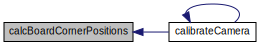
\includegraphics[width=350pt]{main_8cpp_a0a7f48017dbb3d64bfc1a171631ad7d7_icgraph}
\end{center}
\end{figure}
\mbox{\Hypertarget{main_8cpp_a5f7c5996cd5a271d0277e0741f73a5b4}\label{main_8cpp_a5f7c5996cd5a271d0277e0741f73a5b4}} 
\index{main.\+cpp@{main.\+cpp}!calibrate\+Camera@{calibrate\+Camera}}
\index{calibrate\+Camera@{calibrate\+Camera}!main.\+cpp@{main.\+cpp}}
\subsubsection{\texorpdfstring{calibrate\+Camera()}{calibrateCamera()}}
{\footnotesize\ttfamily int calibrate\+Camera (\begin{DoxyParamCaption}{ }\end{DoxyParamCaption})}



Start the camera calibration routine that computes the camera matrix and distortion coefficients. 



Definition at line 769 of file main.\+cpp.


\begin{DoxyCode}
770 \{
771     \hyperlink{main_8cpp_af29e7fc07ae0979d5fb61b473241d33d}{commObj}.\hyperlink{classcomm_object_aec354c7099b3039083cc4224e071e022}{addLog}(\textcolor{stringliteral}{"Started camera calibration. 80 pictures are going to be captured."});
772     CameraLibrary\_EnableDevelopment();
773 \textcolor{comment}{}
774 \textcolor{comment}{    //! Initialize Camera SDK ==--}
775 \textcolor{comment}{}    CameraLibrary::CameraManager::X();
776 \textcolor{comment}{}
777 \textcolor{comment}{    //! At this point the Camera SDK is actively looking for all connected cameras and will initialize}
778 \textcolor{comment}{    //! them on it's own.}
779 \textcolor{comment}{}\textcolor{comment}{}
780 \textcolor{comment}{    //! Get a connected camera ================----}
781 \textcolor{comment}{}    CameraManager::X().WaitForInitialization();
782 
783     Camera *camera = CameraManager::X().GetCamera();
784     \textcolor{keywordflow}{if} (camera == 0)
785     \{
786         \hyperlink{main_8cpp_af29e7fc07ae0979d5fb61b473241d33d}{commObj}.\hyperlink{classcomm_object_aec354c7099b3039083cc4224e071e022}{addLog}(\textcolor{stringliteral}{"No camera found!"});
787         \textcolor{keywordflow}{return} 1;
788     \}
789 \textcolor{comment}{}
790 \textcolor{comment}{    //! Determine camera resolution}
791 \textcolor{comment}{}    \textcolor{keywordtype}{int} cameraWidth = camera->Width();
792     \textcolor{keywordtype}{int} cameraHeight = camera->Height();
793 \textcolor{comment}{}
794 \textcolor{comment}{    //! Set Video Mode ==--}
795 \textcolor{comment}{}\textcolor{comment}{}
796 \textcolor{comment}{    //! We set the camera to Segment Mode here.  This mode is support by all of our products.}
797 \textcolor{comment}{    //! Depending on what device you have connected you might want to consider a different}
798 \textcolor{comment}{    //! video mode to achieve the best possible tracking quality.  All devices that support a}
799 \textcolor{comment}{    //! mode that will achieve a better quality output with a mode other than Segment Mode are}
800 \textcolor{comment}{    //! listed here along with what mode you should use if you're looking for the best head}
801 \textcolor{comment}{    //! tracking:}
802 \textcolor{comment}{    //!}
803 \textcolor{comment}{    //!     V100:R1/R2    Precision Mode}
804 \textcolor{comment}{    //!     TrackIR 5     Bit-Packed Precision Mode}
805 \textcolor{comment}{    //!     V120          Precision Mode}
806 \textcolor{comment}{    //!     TBar          Precision Mode}
807 \textcolor{comment}{    //!     S250e         Precision Mode}
808 \textcolor{comment}{    //!}
809 \textcolor{comment}{    //! If you have questions about a new device that might be conspicuously missing here or}
810 \textcolor{comment}{    //! have any questions about head tracking, email support or participate in our forums.}
811 \textcolor{comment}{}
812     camera->SetVideoType(Core::GrayscaleMode);
813 \textcolor{comment}{}
814 \textcolor{comment}{    //! Start camera output ==--}
815 \textcolor{comment}{}    camera->Start();
816 \textcolor{comment}{}
817 \textcolor{comment}{    //! Camera Matrix creation  ==--}
818 \textcolor{comment}{}    \hyperlink{main_8cpp_a53e8957a459b639ca82d938157f3b085}{cameraMatrix} = Mat::eye(3, 3, CV\_64F);
819     \hyperlink{main_8cpp_a8d67876da148be9118bba1c0d017fb57}{distCoeffs} = Mat::zeros(8, 1, CV\_64F);
820 \textcolor{comment}{}
821 \textcolor{comment}{    //! Ok, start main loop.  This loop fetches and displays   ===---}
822 \textcolor{comment}{    //! camera frames.                                         ===---}
823 \textcolor{comment}{    //! But first set some camera parameters}
824 \textcolor{comment}{}    camera->SetAGC(\textcolor{keyword}{false});
825     camera->SetAEC(\textcolor{keyword}{false});
826     camera->SetExposure(200);
827     camera->SetIntensity(4);
828     camera->SetFrameRate(30);
829     camera->SetIRFilter(\textcolor{keyword}{true});
830     camera->SetContinuousIR(\textcolor{keyword}{false});
831     camera->SetHighPowerMode(\textcolor{keyword}{false});
832 
833     \textcolor{keywordtype}{int} number\_samples = 0;
834     \textcolor{keywordtype}{int} imagesToSample = 80;
835 
836     std::vector<std::vector<Point2f> > imagePoints;
837     std::vector<Point2f> pointBuf;
838     \textcolor{keywordtype}{bool} found;
839     Size boardSize(9, 6);
840     Size imageSize(cameraWidth, cameraHeight);
841     Mat \hyperlink{main_8cpp_ae095f10a005e68d20233dc15b4077ca6}{Rvec}(3, 1, DataType<double>::type);
842     Mat \hyperlink{main_8cpp_a9215ba881de0242c883e5b065d6d2ff9}{Tvec}(3, 1, DataType<double>::type);
843 \textcolor{comment}{}
844 \textcolor{comment}{    //! the user has to provide the size of one square in mm}
845 \textcolor{comment}{}    \textcolor{keywordtype}{bool} ok;
846     \textcolor{keywordtype}{int} qsquareSize = QInputDialog::getInt(\textcolor{keyword}{nullptr}, \textcolor{stringliteral}{"Chessboard size in mm"}, \textcolor{stringliteral}{"Chessboard size in mm"}, 23, 1
      , 60, 1, &ok);
847     \textcolor{keywordtype}{float} squareSize = 23;
848 
849     \textcolor{keywordflow}{if} (ok)
850     \{
851         squareSize = qsquareSize;
852     \}
853 
854     QPixmap QPFrame;
855     \hyperlink{main_8cpp_af29e7fc07ae0979d5fb61b473241d33d}{commObj}.\hyperlink{classcomm_object_acfc97f4310e2b7d841ecb8cf8be0088e}{progressUpdate}(0);
856     \textcolor{keywordflow}{while} (number\_samples < imagesToSample)
857     \{\textcolor{comment}{}
858 \textcolor{comment}{        //! Fetch a new frame from the camera ===---}
859 \textcolor{comment}{}        cv::Mat matFrame(cv::Size(cameraWidth, cameraHeight), CV\_8UC1);
860 \textcolor{comment}{}
861 \textcolor{comment}{        //! which is why we also set this constant to 8 }
862 \textcolor{comment}{}        \textcolor{keyword}{const} \textcolor{keywordtype}{int} \hyperlink{main_8cpp_ae144f2eb508ffc763c259d875c600ab2}{BACKBUFFER\_BITSPERPIXEL} = 8;
863 \textcolor{comment}{}
864 \textcolor{comment}{        //! later on, when we get the frame as usual:}
865 \textcolor{comment}{}        CameraLibrary::Frame * frame = camera->GetFrame();
866 
867         \textcolor{keywordflow}{if} (frame)
868         \{\textcolor{comment}{}
869 \textcolor{comment}{            //! Lets have the Camera Library raster the camera's}
870 \textcolor{comment}{            //! image into our texture.}
871 \textcolor{comment}{}
872             frame->Rasterize(cameraWidth, cameraHeight, matFrame.step, BACKBUFFER\_BITSPERPIXEL, matFrame.
      data);
873             QPFrame = \hyperlink{main_8cpp_a3e3cc959a7ab6f93ea52863d86373ce5}{Mat2QPixmap}(matFrame);
874             \hyperlink{main_8cpp_af29e7fc07ae0979d5fb61b473241d33d}{commObj}.\hyperlink{classcomm_object_a6f81522c2aa1668fa402f08710e6206b}{changeImage}(QPFrame);
875             found = findChessboardCorners(matFrame, boardSize, pointBuf, CV\_CALIB\_CB\_ADAPTIVE\_THRESH | 
      CV\_CALIB\_CB\_FAST\_CHECK | CV\_CALIB\_CB\_NORMALIZE\_IMAGE);
876 
877             \textcolor{keywordflow}{if} (found)                \textcolor{comment}{//!< If done with success,}
878 \textcolor{comment}{}            \{\textcolor{comment}{}
879 \textcolor{comment}{                //! improve the found corners' coordinate accuracy for chessboard}
880 \textcolor{comment}{}                cornerSubPix(matFrame, pointBuf, Size(11, 11), Size(-1, -1), TermCriteria(CV\_TERMCRIT\_EPS +
       CV\_TERMCRIT\_ITER, 30, 0.1));
881 
882                 imagePoints.push\_back(pointBuf);
883                 number\_samples += 1;
884                 \hyperlink{main_8cpp_af29e7fc07ae0979d5fb61b473241d33d}{commObj}.\hyperlink{classcomm_object_aec354c7099b3039083cc4224e071e022}{addLog}(QString::fromStdString(\hyperlink{main_8cpp_a8fc3524f4e679a41dcc8d0f302d637ed}{ss}.str()));
885                 QCoreApplication::processEvents();
886             \}
887             frame->Release();
888             \hyperlink{main_8cpp_a8fc3524f4e679a41dcc8d0f302d637ed}{ss}.str(\textcolor{stringliteral}{""});
889             \hyperlink{main_8cpp_a8fc3524f4e679a41dcc8d0f302d637ed}{ss} << \textcolor{stringliteral}{"Samples found  =  "} << number\_samples;
890             \hyperlink{main_8cpp_af29e7fc07ae0979d5fb61b473241d33d}{commObj}.\hyperlink{classcomm_object_acfc97f4310e2b7d841ecb8cf8be0088e}{progressUpdate}(number\_samples * 100 / imagesToSample);
891         \}
892         Sleep(2);
893     \}
894 
895     std::vector<std::vector<Point3f> > objectPoints(1);
896     \hyperlink{main_8cpp_a0a7f48017dbb3d64bfc1a171631ad7d7}{calcBoardCornerPositions}(boardSize, squareSize, objectPoints[0]);
897     objectPoints.resize(imagePoints.size(), objectPoints[0]);
898 
899     \textcolor{keywordtype}{double} rms = \hyperlink{main_8cpp_a5f7c5996cd5a271d0277e0741f73a5b4}{calibrateCamera}(objectPoints, imagePoints, imageSize, 
      \hyperlink{main_8cpp_a53e8957a459b639ca82d938157f3b085}{cameraMatrix}, \hyperlink{main_8cpp_a8d67876da148be9118bba1c0d017fb57}{distCoeffs}, \hyperlink{main_8cpp_ae095f10a005e68d20233dc15b4077ca6}{Rvec}, \hyperlink{main_8cpp_a9215ba881de0242c883e5b065d6d2ff9}{Tvec});
900     \hyperlink{main_8cpp_af29e7fc07ae0979d5fb61b473241d33d}{commObj}.\hyperlink{classcomm_object_acfc97f4310e2b7d841ecb8cf8be0088e}{progressUpdate}(0);\textcolor{comment}{}
901 \textcolor{comment}{    //! Release camera ==--}
902 \textcolor{comment}{}    camera->Release();
903 \textcolor{comment}{}
904 \textcolor{comment}{    //! Save the obtained calibration coefficients in a file for later use}
905 \textcolor{comment}{}    QString fileName = QFileDialog::getSaveFileName(\textcolor{keyword}{nullptr}, \textcolor{stringliteral}{"Save calibration file"}, \textcolor{stringliteral}{""}, \textcolor{stringliteral}{"Calibration File
       (*.xml);;All Files (*)"});
906     FileStorage fs(fileName.toUtf8().constData(), FileStorage::WRITE);
907     fs << \textcolor{stringliteral}{"CameraMatrix"} << \hyperlink{main_8cpp_a53e8957a459b639ca82d938157f3b085}{cameraMatrix};
908     fs << \textcolor{stringliteral}{"DistCoeff"} << \hyperlink{main_8cpp_a8d67876da148be9118bba1c0d017fb57}{distCoeffs};
909     fs << \textcolor{stringliteral}{"RMS"} << rms;
910     \hyperlink{main_8cpp_a7b795a27447192fa68ef7c2d8ee1adab}{strBuf} = fs.releaseAndGetString();
911     \hyperlink{main_8cpp_af29e7fc07ae0979d5fb61b473241d33d}{commObj}.\hyperlink{classcomm_object_a1f4b8dd22ecc46bab619f6b1fe1a5144}{changeStatus}(QString::fromStdString(\hyperlink{main_8cpp_a7b795a27447192fa68ef7c2d8ee1adab}{strBuf}));
912     \hyperlink{main_8cpp_af29e7fc07ae0979d5fb61b473241d33d}{commObj}.\hyperlink{classcomm_object_aec354c7099b3039083cc4224e071e022}{addLog}(\textcolor{stringliteral}{"Saved calibration!"});
913     \textcolor{keywordflow}{return} 0;
914 \}
\end{DoxyCode}
Here is the call graph for this function\+:\nopagebreak
\begin{figure}[H]
\begin{center}
\leavevmode
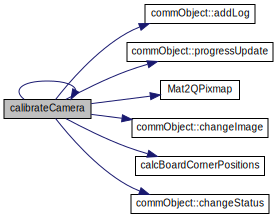
\includegraphics[width=341pt]{main_8cpp_a5f7c5996cd5a271d0277e0741f73a5b4_cgraph}
\end{center}
\end{figure}
Here is the caller graph for this function\+:\nopagebreak
\begin{figure}[H]
\begin{center}
\leavevmode
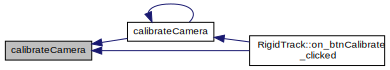
\includegraphics[width=350pt]{main_8cpp_a5f7c5996cd5a271d0277e0741f73a5b4_icgraph}
\end{center}
\end{figure}
\mbox{\Hypertarget{main_8cpp_a7ad2e3cfb5056dbab2098e0dd3bd353f}\label{main_8cpp_a7ad2e3cfb5056dbab2098e0dd3bd353f}} 
\index{main.\+cpp@{main.\+cpp}!calibrate\+Ground@{calibrate\+Ground}}
\index{calibrate\+Ground@{calibrate\+Ground}!main.\+cpp@{main.\+cpp}}
\subsubsection{\texorpdfstring{calibrate\+Ground()}{calibrateGround()}}
{\footnotesize\ttfamily int calibrate\+Ground (\begin{DoxyParamCaption}{ }\end{DoxyParamCaption})}

Get the pose of the camera w.\+r.\+t the ground calibration frame. This frame sets the navigation frame for later results. The pose is averaged over 200 samples and then saved in the file reference\+Data.\+xml. This routine is basically the same as set\+Reference. 

Definition at line 1558 of file main.\+cpp.


\begin{DoxyCode}
1559 \{\textcolor{comment}{}
1560 \textcolor{comment}{    //! initialize the variables with starting values}
1561 \textcolor{comment}{}    \hyperlink{main_8cpp_acf655f393e3996144226399a338e8d3b}{gotOrder} = \textcolor{keyword}{false};
1562     \hyperlink{main_8cpp_a9d2e25dbfda0ebcdbb488652c8b15fad}{posRef} = 0;
1563     \hyperlink{main_8cpp_acd6966c004a57c4080ba204152200e7f}{eulerRef} = 0;
1564     \hyperlink{main_8cpp_a4ee4d2abbe47b92c21b81c5c4389086e}{RmatRef} = 0;
1565     \hyperlink{main_8cpp_ae095f10a005e68d20233dc15b4077ca6}{Rvec} = \hyperlink{main_8cpp_ae101daeaec726e27690c862b7edea825}{RvecOriginal};
1566     \hyperlink{main_8cpp_a9215ba881de0242c883e5b065d6d2ff9}{Tvec} = \hyperlink{main_8cpp_a043bf1deaf5d42d47e0cce8982c1f18b}{TvecOriginal};
1567 
1568     \hyperlink{main_8cpp_a0416912fce6274568e80019b10ba294f}{determineExposure}();
1569 
1570     \hyperlink{main_8cpp_a8fc3524f4e679a41dcc8d0f302d637ed}{ss}.str(\textcolor{stringliteral}{""});
1571     \hyperlink{main_8cpp_af29e7fc07ae0979d5fb61b473241d33d}{commObj}.\hyperlink{classcomm_object_aec354c7099b3039083cc4224e071e022}{addLog}(\textcolor{stringliteral}{"Started ground calibration"});
1572 
1573     CameraLibrary\_EnableDevelopment();\textcolor{comment}{}
1574 \textcolor{comment}{    //! Initialize Camera SDK ==--}
1575 \textcolor{comment}{}    CameraLibrary::CameraManager::X();
1576 \textcolor{comment}{}
1577 \textcolor{comment}{    //! At this point the Camera SDK is actively looking for all connected cameras and will initialize}
1578 \textcolor{comment}{    //! them on it's own.}
1579 \textcolor{comment}{}\textcolor{comment}{}
1580 \textcolor{comment}{    //! Get a connected camera ================----}
1581 \textcolor{comment}{}    CameraManager::X().WaitForInitialization();
1582     Camera *camera = CameraManager::X().GetCamera();
1583 \textcolor{comment}{}
1584 \textcolor{comment}{    //! If no device connected, pop a message box and exit ==--}
1585 \textcolor{comment}{}    \textcolor{keywordflow}{if} (camera == 0)
1586     \{
1587         \hyperlink{main_8cpp_af29e7fc07ae0979d5fb61b473241d33d}{commObj}.\hyperlink{classcomm_object_aec354c7099b3039083cc4224e071e022}{addLog}(\textcolor{stringliteral}{"No camera found!"});
1588         \textcolor{keywordflow}{return} 1;
1589     \}
1590 \textcolor{comment}{}
1591 \textcolor{comment}{    //! Determine camera resolution to size application window ==----}
1592 \textcolor{comment}{}    \textcolor{keywordtype}{int} cameraWidth = camera->Width();
1593     \textcolor{keywordtype}{int} cameraHeight = camera->Height();
1594     camera->GetDistortionModel(\hyperlink{main_8cpp_a9fba099569a2da23e458c2571f69652a}{distModel});
1595     cv::Mat matFrame(cv::Size(cameraWidth, cameraHeight), CV\_8UC1);
1596 \textcolor{comment}{}
1597 \textcolor{comment}{    //! Set camera mode to precision mode, it directly provides marker coordinates}
1598 \textcolor{comment}{}    camera->SetVideoType(Core::PrecisionMode);
1599 \textcolor{comment}{}
1600 \textcolor{comment}{    //! Start camera output ==--}
1601 \textcolor{comment}{}    camera->Start();
1602 \textcolor{comment}{}
1603 \textcolor{comment}{    //! Turn on some overlay text so it's clear things are     ===---}
1604 \textcolor{comment}{    //! working even if there is nothing in the camera's view. ===---}
1605 \textcolor{comment}{    //! Set some other parameters as well of the camera}
1606 \textcolor{comment}{}    camera->SetTextOverlay(\textcolor{keyword}{true});
1607     camera->SetFrameRate(\hyperlink{main_8cpp_aa5b833b78b107a1a04eb4edba151c0ba}{intFrameRate});
1608     camera->SetIntensity(\hyperlink{main_8cpp_a4e18b0b26ecc511ca7d2f2205313e537}{intIntensity});
1609     camera->SetIRFilter(\textcolor{keyword}{true});
1610     camera->SetContinuousIR(\textcolor{keyword}{false});
1611     camera->SetHighPowerMode(\textcolor{keyword}{false});
1612 \textcolor{comment}{}
1613 \textcolor{comment}{    //! sample some frames and calculate the position and attitude. then average those values and use that
       as zero position}
1614 \textcolor{comment}{}    \textcolor{keywordtype}{int} numberSamples = 0;
1615     \textcolor{keywordtype}{int} numberToSample = 200;
1616     \textcolor{keywordtype}{double} projectionError = 0;
1617 
1618     \textcolor{keywordflow}{while} (numberSamples < numberToSample)
1619     \{\textcolor{comment}{}
1620 \textcolor{comment}{        //! Fetch a new frame from the camera ===---}
1621 \textcolor{comment}{}        Frame *frame = camera->GetFrame();
1622 
1623         \textcolor{keywordflow}{if} (frame)
1624         \{\textcolor{comment}{}
1625 \textcolor{comment}{            //! Ok, we've received a new frame, lets do something}
1626 \textcolor{comment}{            //! with it.}
1627 \textcolor{comment}{}            \textcolor{keywordflow}{if} (frame->ObjectCount() == \hyperlink{main_8cpp_ae1d37a43f631aefe76b6e540da786064}{numberMarkers})
1628             \{\textcolor{comment}{}
1629 \textcolor{comment}{                //!for(int i=0; i<frame->ObjectCount(); i++)}
1630 \textcolor{comment}{}                \textcolor{keywordflow}{for} (\textcolor{keywordtype}{int} i = 0; i < \hyperlink{main_8cpp_ae1d37a43f631aefe76b6e540da786064}{numberMarkers}; i++)
1631                 \{
1632                     cObject *obj = frame->Object(i);
1633                     \hyperlink{main_8cpp_a54cb682bd037283c18b5a9a447ff5e5e}{list\_points2dUnsorted}[i] = cv::Point2d(obj->X(), obj->Y());
1634                 \}
1635 
1636                 \textcolor{keywordflow}{if} (\hyperlink{main_8cpp_acf655f393e3996144226399a338e8d3b}{gotOrder} == \textcolor{keyword}{false})
1637                 \{
1638                     \hyperlink{main_8cpp_a11ff459289305229597defd39f510959}{determineOrder}();
1639                 \}
1640 \textcolor{comment}{}
1641 \textcolor{comment}{                //! sort the 2d points with the correct indices as found in the preceeding order
       determination algorithm}
1642 \textcolor{comment}{}                \textcolor{keywordflow}{for} (\textcolor{keywordtype}{int} w = 0; w < \hyperlink{main_8cpp_ae1d37a43f631aefe76b6e540da786064}{numberMarkers}; w++)
1643                 \{
1644                     \hyperlink{main_8cpp_ad583e75f176dafdb7de3f214673851de}{list\_points2d}[w] = \hyperlink{main_8cpp_a54cb682bd037283c18b5a9a447ff5e5e}{list\_points2dUnsorted}[
      \hyperlink{main_8cpp_ac06fee052099b9fc9f0826315bb64a4a}{pointOrderIndices}[w]];
1645                 \}
1646                 \hyperlink{main_8cpp_a85d3d8c8a0e3e9cfb6157c247470d934}{list\_points2dOld} = \hyperlink{main_8cpp_a54cb682bd037283c18b5a9a447ff5e5e}{list\_points2dUnsorted};
1647 \textcolor{comment}{}
1648 \textcolor{comment}{                //!Compute the pose from the 3D-2D corresponses}
1649 \textcolor{comment}{}                solvePnP(\hyperlink{main_8cpp_a933edb4ba1c0589d59020164c2f1ff87}{list\_points3d}, \hyperlink{main_8cpp_ad583e75f176dafdb7de3f214673851de}{list\_points2d}, 
      \hyperlink{main_8cpp_a53e8957a459b639ca82d938157f3b085}{cameraMatrix}, \hyperlink{main_8cpp_a8d67876da148be9118bba1c0d017fb57}{distCoeffs}, \hyperlink{main_8cpp_ae095f10a005e68d20233dc15b4077ca6}{Rvec}, \hyperlink{main_8cpp_a9215ba881de0242c883e5b065d6d2ff9}{Tvec}, \hyperlink{main_8cpp_ab1cc9be1ff0871bc5de1eb4c2811ae3e}{useGuess}, 
      \hyperlink{main_8cpp_ab5e634b66221f494504aea1557af5df9}{methodPNP});
1650 \textcolor{comment}{}
1651 \textcolor{comment}{                //! project the marker 3d points with the solution into the camera image CoSy and calculate
       difference to true camera image}
1652 \textcolor{comment}{}                projectPoints(\hyperlink{main_8cpp_a933edb4ba1c0589d59020164c2f1ff87}{list\_points3d}, \hyperlink{main_8cpp_ae095f10a005e68d20233dc15b4077ca6}{Rvec}, \hyperlink{main_8cpp_a9215ba881de0242c883e5b065d6d2ff9}{Tvec}, 
      \hyperlink{main_8cpp_a53e8957a459b639ca82d938157f3b085}{cameraMatrix}, \hyperlink{main_8cpp_a8d67876da148be9118bba1c0d017fb57}{distCoeffs}, \hyperlink{main_8cpp_a7b88d0425a68875639d40a17079df819}{list\_points2dProjected});
1653                 projectionError = norm(\hyperlink{main_8cpp_a7b88d0425a68875639d40a17079df819}{list\_points2dProjected}, 
      \hyperlink{main_8cpp_ad583e75f176dafdb7de3f214673851de}{list\_points2d});
1654 
1655                 \textcolor{keywordflow}{if} (projectionError > 3)
1656                 \{
1657                     \hyperlink{main_8cpp_af29e7fc07ae0979d5fb61b473241d33d}{commObj}.\hyperlink{classcomm_object_aec354c7099b3039083cc4224e071e022}{addLog}(\textcolor{stringliteral}{"Reprojection error is bigger than 3 pixel. Correct marker
       configuration loaded?\(\backslash\)nMarker position measured precisely?"});
1658                     frame->Release();
1659                     \textcolor{keywordflow}{return} 1;
1660                 \}
1661 
1662                 \textcolor{keywordtype}{double} maxValue = 0;
1663                 \textcolor{keywordtype}{double} minValue = 0;
1664                 minMaxLoc(\hyperlink{main_8cpp_a9215ba881de0242c883e5b065d6d2ff9}{Tvec}.at<\textcolor{keywordtype}{double}>(2), &minValue, &maxValue);
1665 
1666                 \textcolor{keywordflow}{if} (maxValue > 10000 || minValue < 0)
1667                 \{
1668 
1669 
1670                     \hyperlink{main_8cpp_af29e7fc07ae0979d5fb61b473241d33d}{commObj}.\hyperlink{classcomm_object_aec354c7099b3039083cc4224e071e022}{addLog}(\textcolor{stringliteral}{"Negative z distance, thats not possible. Start the set
       zero routine again and check marker configurations."});
1671                     frame->Release();
1672                     \textcolor{keywordflow}{return} 1;
1673                 \}
1674 
1675                 \textcolor{keywordflow}{if} (norm(\hyperlink{main_8cpp_a1d543a183197268bcb54a06bf157852c}{positionOld}) - norm(\hyperlink{main_8cpp_a9215ba881de0242c883e5b065d6d2ff9}{Tvec}) < 0.05)   \textcolor{comment}{//!<Iterative Method needs time
       to converge to solution}
1676 \textcolor{comment}{}                \{
1677                     add(\hyperlink{main_8cpp_a9d2e25dbfda0ebcdbb488652c8b15fad}{posRef}, \hyperlink{main_8cpp_a9215ba881de0242c883e5b065d6d2ff9}{Tvec}, \hyperlink{main_8cpp_a9d2e25dbfda0ebcdbb488652c8b15fad}{posRef});
1678                     add(\hyperlink{main_8cpp_acd6966c004a57c4080ba204152200e7f}{eulerRef}, \hyperlink{main_8cpp_ae095f10a005e68d20233dc15b4077ca6}{Rvec}, \hyperlink{main_8cpp_acd6966c004a57c4080ba204152200e7f}{eulerRef}); \textcolor{comment}{//!< That are not the values of yaw,
       roll and pitch yet! Rodriguez has to be called first. }
1679 \textcolor{comment}{}                    numberSamples++;    \textcolor{comment}{//!<-- one sample more :D}
1680 \textcolor{comment}{}                    \hyperlink{main_8cpp_af29e7fc07ae0979d5fb61b473241d33d}{commObj}.\hyperlink{classcomm_object_acfc97f4310e2b7d841ecb8cf8be0088e}{progressUpdate}(numberSamples * 100 / numberToSample);
1681                 \}
1682                 \hyperlink{main_8cpp_a1d543a183197268bcb54a06bf157852c}{positionOld} = \hyperlink{main_8cpp_a9215ba881de0242c883e5b065d6d2ff9}{Tvec};
1683 
1684                 Mat cFrame(480, 640, CV\_8UC3, Scalar(0, 0, 0));
1685                 \textcolor{keywordflow}{for} (\textcolor{keywordtype}{int} i = 0; i < \hyperlink{main_8cpp_ae1d37a43f631aefe76b6e540da786064}{numberMarkers}; i++)
1686                 \{
1687                     circle(cFrame, Point(\hyperlink{main_8cpp_ad583e75f176dafdb7de3f214673851de}{list\_points2d}[i].x, 
      \hyperlink{main_8cpp_ad583e75f176dafdb7de3f214673851de}{list\_points2d}[i].y), 6, Scalar(0, 225, 0), 3);
1688                 \}
1689                 \hyperlink{main_8cpp_a2104a5d9d6b9f1e29bc4cd858c59882e}{projectCoordinateFrame}(cFrame);
1690                 projectPoints(\hyperlink{main_8cpp_a933edb4ba1c0589d59020164c2f1ff87}{list\_points3d}, \hyperlink{main_8cpp_ae095f10a005e68d20233dc15b4077ca6}{Rvec}, \hyperlink{main_8cpp_a9215ba881de0242c883e5b065d6d2ff9}{Tvec}, 
      \hyperlink{main_8cpp_a53e8957a459b639ca82d938157f3b085}{cameraMatrix}, \hyperlink{main_8cpp_a8d67876da148be9118bba1c0d017fb57}{distCoeffs}, \hyperlink{main_8cpp_ad583e75f176dafdb7de3f214673851de}{list\_points2d});
1691                 \textcolor{keywordflow}{for} (\textcolor{keywordtype}{int} i = 0; i < \hyperlink{main_8cpp_ae1d37a43f631aefe76b6e540da786064}{numberMarkers}; i++)
1692                 \{
1693                     circle(cFrame, Point(\hyperlink{main_8cpp_ad583e75f176dafdb7de3f214673851de}{list\_points2d}[i].x, 
      \hyperlink{main_8cpp_ad583e75f176dafdb7de3f214673851de}{list\_points2d}[i].y), 3, Scalar(225, 0, 0), 3);
1694                 \}
1695 
1696                 QPixmap QPFrame;
1697                 QPFrame = \hyperlink{main_8cpp_a3e3cc959a7ab6f93ea52863d86373ce5}{Mat2QPixmap}(cFrame);
1698                 \hyperlink{main_8cpp_af29e7fc07ae0979d5fb61b473241d33d}{commObj}.\hyperlink{classcomm_object_a6f81522c2aa1668fa402f08710e6206b}{changeImage}(QPFrame);
1699                 QCoreApplication::processEvents();
1700 
1701             \}
1702             frame->Release();
1703         \}
1704     \}\textcolor{comment}{}
1705 \textcolor{comment}{    //! Release camera ==--}
1706 \textcolor{comment}{}    camera->Release();
1707 \textcolor{comment}{}
1708 \textcolor{comment}{    //!Divide by the number of samples to get the mean of the reference position}
1709 \textcolor{comment}{}    divide(\hyperlink{main_8cpp_a9d2e25dbfda0ebcdbb488652c8b15fad}{posRef}, numberToSample, \hyperlink{main_8cpp_a9d2e25dbfda0ebcdbb488652c8b15fad}{posRef});
1710     divide(\hyperlink{main_8cpp_acd6966c004a57c4080ba204152200e7f}{eulerRef}, numberToSample, \hyperlink{main_8cpp_acd6966c004a57c4080ba204152200e7f}{eulerRef}); \textcolor{comment}{//!< eulerRef is here in Axis Angle
       notation}
1711 \textcolor{comment}{}
1712     Rodrigues(\hyperlink{main_8cpp_acd6966c004a57c4080ba204152200e7f}{eulerRef}, \hyperlink{main_8cpp_a4ee4d2abbe47b92c21b81c5c4389086e}{RmatRef});                \textcolor{comment}{//!< axis angle to rotation matrix}
1713 \textcolor{comment}{}
1714     \hyperlink{main_8cpp_ab2b71933055cf32cc8e5e2100fd7723f}{getEulerAngles}(\hyperlink{main_8cpp_a4ee4d2abbe47b92c21b81c5c4389086e}{RmatRef}, \hyperlink{main_8cpp_acd6966c004a57c4080ba204152200e7f}{eulerRef}); \textcolor{comment}{//!<  rotation matrix to euler}
1715 \textcolor{comment}{}    \hyperlink{main_8cpp_a8fc3524f4e679a41dcc8d0f302d637ed}{ss}.str(\textcolor{stringliteral}{""});
1716     \hyperlink{main_8cpp_a8fc3524f4e679a41dcc8d0f302d637ed}{ss} << \textcolor{stringliteral}{"RmatRef is:\(\backslash\)n"};
1717     \hyperlink{main_8cpp_a8fc3524f4e679a41dcc8d0f302d637ed}{ss} << \hyperlink{main_8cpp_a4ee4d2abbe47b92c21b81c5c4389086e}{RmatRef} << \textcolor{stringliteral}{"\(\backslash\)n"};
1718     \hyperlink{main_8cpp_a8fc3524f4e679a41dcc8d0f302d637ed}{ss} << \textcolor{stringliteral}{"Reference Position is:\(\backslash\)n"};
1719     \hyperlink{main_8cpp_a8fc3524f4e679a41dcc8d0f302d637ed}{ss} << \hyperlink{main_8cpp_a9d2e25dbfda0ebcdbb488652c8b15fad}{posRef} << \textcolor{stringliteral}{"[mm] \(\backslash\)n"};
1720     \hyperlink{main_8cpp_a8fc3524f4e679a41dcc8d0f302d637ed}{ss} << \textcolor{stringliteral}{"Reference Euler angles are:\(\backslash\)n"};
1721     \hyperlink{main_8cpp_a8fc3524f4e679a41dcc8d0f302d637ed}{ss} << \hyperlink{main_8cpp_acd6966c004a57c4080ba204152200e7f}{eulerRef} << \textcolor{stringliteral}{"[deg] \(\backslash\)n"};
1722 \textcolor{comment}{}
1723 \textcolor{comment}{    //! Save the obtained calibration coefficients in a file for later use}
1724 \textcolor{comment}{}    QString fileName = QFileDialog::getSaveFileName(\textcolor{keyword}{nullptr}, \textcolor{stringliteral}{"Save ground calibration file"}, \textcolor{stringliteral}{"
      referenceData.xml"}, \textcolor{stringliteral}{"Calibration File (*.xml);;All Files (*)"});
1725     FileStorage fs(fileName.toUtf8().constData(), FileStorage::WRITE);
1726     fs << \textcolor{stringliteral}{"M\_NC"} << \hyperlink{main_8cpp_a4ee4d2abbe47b92c21b81c5c4389086e}{RmatRef};
1727     fs << \textcolor{stringliteral}{"eulerRef"} << \hyperlink{main_8cpp_acd6966c004a57c4080ba204152200e7f}{eulerRef};
1728     \hyperlink{main_8cpp_a7b795a27447192fa68ef7c2d8ee1adab}{strBuf} = fs.releaseAndGetString();
1729     \hyperlink{main_8cpp_af29e7fc07ae0979d5fb61b473241d33d}{commObj}.\hyperlink{classcomm_object_a1f4b8dd22ecc46bab619f6b1fe1a5144}{changeStatus}(QString::fromStdString(\hyperlink{main_8cpp_a7b795a27447192fa68ef7c2d8ee1adab}{strBuf}));
1730     \hyperlink{main_8cpp_af29e7fc07ae0979d5fb61b473241d33d}{commObj}.\hyperlink{classcomm_object_aec354c7099b3039083cc4224e071e022}{addLog}(\textcolor{stringliteral}{"Saved ground calibration!"});
1731     \hyperlink{main_8cpp_af29e7fc07ae0979d5fb61b473241d33d}{commObj}.\hyperlink{classcomm_object_acfc97f4310e2b7d841ecb8cf8be0088e}{progressUpdate}(0);
1732     \textcolor{keywordflow}{return} 0;
1733 \}
\end{DoxyCode}
Here is the call graph for this function\+:\nopagebreak
\begin{figure}[H]
\begin{center}
\leavevmode
\includegraphics[width=350pt]{main_8cpp_a7ad2e3cfb5056dbab2098e0dd3bd353f_cgraph}
\end{center}
\end{figure}
Here is the caller graph for this function\+:\nopagebreak
\begin{figure}[H]
\begin{center}
\leavevmode
\includegraphics[width=337pt]{main_8cpp_a7ad2e3cfb5056dbab2098e0dd3bd353f_icgraph}
\end{center}
\end{figure}
\mbox{\Hypertarget{main_8cpp_af2a8b7de0b15dc17198c147ba39e85f3}\label{main_8cpp_af2a8b7de0b15dc17198c147ba39e85f3}} 
\index{main.\+cpp@{main.\+cpp}!close\+U\+DP@{close\+U\+DP}}
\index{close\+U\+DP@{close\+U\+DP}!main.\+cpp@{main.\+cpp}}
\subsubsection{\texorpdfstring{close\+U\+D\+P()}{closeUDP()}}
{\footnotesize\ttfamily void close\+U\+DP (\begin{DoxyParamCaption}{ }\end{DoxyParamCaption})}

Close the U\+DP ports again to release network interfaces etc. If this is not done the network resources are still occupied and the program can\textquotesingle{}t exit properly. 

Definition at line 1168 of file main.\+cpp.


\begin{DoxyCode}
1169 \{\textcolor{comment}{}
1170 \textcolor{comment}{    //! check if the socket is open and if yes close it}
1171 \textcolor{comment}{}    \textcolor{keywordflow}{if} (\hyperlink{main_8cpp_ae628b9aba095776b7134cf188486e174}{udpSocketObject}->isOpen())
1172     \{
1173         \hyperlink{main_8cpp_ae628b9aba095776b7134cf188486e174}{udpSocketObject}->close();
1174     \}
1175 
1176     \textcolor{keywordflow}{if} (\hyperlink{main_8cpp_a6aa0c3a69dc10d5c4432dcf62e2155d3}{udpSocketSafety}->isOpen())
1177     \{
1178         \hyperlink{main_8cpp_a6aa0c3a69dc10d5c4432dcf62e2155d3}{udpSocketSafety}->close();
1179     \}
1180 
1181     \textcolor{keywordflow}{if} (\hyperlink{main_8cpp_a4260e46da4e0e430642b2d8d8d3c7dd1}{udpSocketSafety2}->isOpen())
1182     \{
1183         \hyperlink{main_8cpp_a4260e46da4e0e430642b2d8d8d3c7dd1}{udpSocketSafety2}->close();
1184     \}
1185     \hyperlink{main_8cpp_af29e7fc07ae0979d5fb61b473241d33d}{commObj}.\hyperlink{classcomm_object_aec354c7099b3039083cc4224e071e022}{addLog}(\textcolor{stringliteral}{"Closed all UDP ports."});
1186 \}
\end{DoxyCode}
Here is the call graph for this function\+:\nopagebreak
\begin{figure}[H]
\begin{center}
\leavevmode
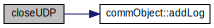
\includegraphics[width=286pt]{main_8cpp_af2a8b7de0b15dc17198c147ba39e85f3_cgraph}
\end{center}
\end{figure}
Here is the caller graph for this function\+:\nopagebreak
\begin{figure}[H]
\begin{center}
\leavevmode
\includegraphics[width=350pt]{main_8cpp_af2a8b7de0b15dc17198c147ba39e85f3_icgraph}
\end{center}
\end{figure}
\mbox{\Hypertarget{main_8cpp_a0416912fce6274568e80019b10ba294f}\label{main_8cpp_a0416912fce6274568e80019b10ba294f}} 
\index{main.\+cpp@{main.\+cpp}!determine\+Exposure@{determine\+Exposure}}
\index{determine\+Exposure@{determine\+Exposure}!main.\+cpp@{main.\+cpp}}
\subsubsection{\texorpdfstring{determine\+Exposure()}{determineExposure()}}
{\footnotesize\ttfamily int determine\+Exposure (\begin{DoxyParamCaption}{ }\end{DoxyParamCaption})}

Get the optimal exposure for the camera. For that find the minimum and maximum exposure were the right number of markers are detected. Then the mean of those two values is used as exposure. 

Definition at line 1357 of file main.\+cpp.


\begin{DoxyCode}
1358 \{\textcolor{comment}{}
1359 \textcolor{comment}{    //! For OptiTrack Ethernet cameras, it's important to enable development mode if you}
1360 \textcolor{comment}{    //! want to stop execution for an extended time while debugging without disconnecting}
1361 \textcolor{comment}{    //! the Ethernet devices.  Lets do that now:}
1362 \textcolor{comment}{}
1363     CameraLibrary\_EnableDevelopment();
1364 \textcolor{comment}{}
1365 \textcolor{comment}{    //! Initialize Camera SDK ==--}
1366 \textcolor{comment}{}    CameraLibrary::CameraManager::X();
1367 \textcolor{comment}{}
1368 \textcolor{comment}{    //! At this point the Camera SDK is actively looking for all connected cameras and will initialize}
1369 \textcolor{comment}{    //! them on it's own.}
1370 \textcolor{comment}{}\textcolor{comment}{}
1371 \textcolor{comment}{    //! Get a connected camera ================----}
1372 \textcolor{comment}{}    CameraManager::X().WaitForInitialization();
1373     Camera *camera = CameraManager::X().GetCamera();
1374 \textcolor{comment}{}
1375 \textcolor{comment}{    //! If no device connected, pop a message box and exit ==--}
1376 \textcolor{comment}{}    \textcolor{keywordflow}{if} (camera == 0)
1377     \{
1378         \hyperlink{main_8cpp_af29e7fc07ae0979d5fb61b473241d33d}{commObj}.\hyperlink{classcomm_object_aec354c7099b3039083cc4224e071e022}{addLog}(\textcolor{stringliteral}{"No camera found!"});
1379         \textcolor{keywordflow}{return} 1;
1380     \}
1381 \textcolor{comment}{}
1382 \textcolor{comment}{    //! Determine camera resolution to size application window ==----}
1383 \textcolor{comment}{}    \textcolor{keywordtype}{int} cameraWidth = camera->Width();
1384     \textcolor{keywordtype}{int} cameraHeight = camera->Height();
1385 
1386     camera->SetVideoType(Core::PrecisionMode);  \textcolor{comment}{//! set the camera mode to precision mode, it used
       greyscale imformation for marker property calculations}
1387 \textcolor{comment}{}\textcolor{comment}{}
1388 \textcolor{comment}{                                                //! Start camera output ==--}
1389 \textcolor{comment}{}    camera->Start();
1390 \textcolor{comment}{}
1391 \textcolor{comment}{    //! Turn on some overlay text so it's clear things are     ===---}
1392 \textcolor{comment}{    //! working even if there is nothing in the camera's view. ===---}
1393 \textcolor{comment}{}    camera->SetTextOverlay(\textcolor{keyword}{true});
1394     camera->SetExposure(\hyperlink{main_8cpp_afcaebd6cfd12b2e558363a06db8396ea}{intExposure});    \textcolor{comment}{//! set the camera exposure}
1395 \textcolor{comment}{}    camera->SetIntensity(\hyperlink{main_8cpp_a4e18b0b26ecc511ca7d2f2205313e537}{intIntensity}); \textcolor{comment}{//! set the camera infrared LED intensity}
1396 \textcolor{comment}{}    camera->SetFrameRate(\hyperlink{main_8cpp_aa5b833b78b107a1a04eb4edba151c0ba}{intFrameRate}); \textcolor{comment}{//! set the camera framerate to 100 Hz}
1397 \textcolor{comment}{}    camera->SetIRFilter(\textcolor{keyword}{true});  \textcolor{comment}{//! enable the filter that blocks visible light and only passes infrared
       light}
1398 \textcolor{comment}{}    camera->SetHighPowerMode(\textcolor{keyword}{true}); \textcolor{comment}{//! enable high power mode of the leds}
1399 \textcolor{comment}{}    camera->SetContinuousIR(\textcolor{keyword}{false}); \textcolor{comment}{//! enable continuous LED light}
1400 \textcolor{comment}{}    camera->SetThreshold(\hyperlink{main_8cpp_ac61559ce6020b8ec00161bc3a994ddcc}{intThreshold}); \textcolor{comment}{//! set threshold for marker detection}
1401 \textcolor{comment}{}\textcolor{comment}{}
1402 \textcolor{comment}{    //!set exposure such that num markers are visible}
1403 \textcolor{comment}{}    \textcolor{keywordtype}{int} numberObjects = 0;  \textcolor{comment}{//! Number of objects (markers) found in the current picture with the given
       exposure    }
1404 \textcolor{comment}{}    \textcolor{keywordtype}{int} minExposure = 1;    \textcolor{comment}{//! exposure when objects detected the first time is numberMarkers }
1405 \textcolor{comment}{}    \textcolor{keywordtype}{int} maxExposure = 480;  \textcolor{comment}{//! exposure when objects detected is first time numberMarkers+1}
1406 \textcolor{comment}{}    \hyperlink{main_8cpp_afcaebd6cfd12b2e558363a06db8396ea}{intExposure} = minExposure;   \textcolor{comment}{//! set the exposure to the smallest value possible}
1407 \textcolor{comment}{}    \textcolor{keywordtype}{int} numberTries = 0;    \textcolor{comment}{//! if the markers arent found after numberTries then there might be no markers
       at all in the real world}
1408 \textcolor{comment}{}\textcolor{comment}{}
1409 \textcolor{comment}{                            //! Determine minimum exposure, hence when are numberMarkers objects detected}
1410 \textcolor{comment}{}    camera->SetExposure(\hyperlink{main_8cpp_afcaebd6cfd12b2e558363a06db8396ea}{intExposure});
1411     \textcolor{keywordflow}{while} (numberObjects != \hyperlink{main_8cpp_ae1d37a43f631aefe76b6e540da786064}{numberMarkers} && numberTries < 48)
1412     \{\textcolor{comment}{}
1413 \textcolor{comment}{        //! get a new camera frame}
1414 \textcolor{comment}{}        Frame *frame = camera->GetFrame();
1415         \textcolor{keywordflow}{if} (frame) \textcolor{comment}{//! frame received}
1416 \textcolor{comment}{}        \{
1417             numberObjects = frame->ObjectCount();   \textcolor{comment}{//! how many objects are detected in the image}
1418 \textcolor{comment}{}            \textcolor{keywordflow}{if} (numberObjects == \hyperlink{main_8cpp_ae1d37a43f631aefe76b6e540da786064}{numberMarkers}) \{ minExposure = 
      \hyperlink{main_8cpp_afcaebd6cfd12b2e558363a06db8396ea}{intExposure}; frame->Release(); \textcolor{keywordflow}{break}; \} \textcolor{comment}{//! if the right amount if markers is found, exit while
       loop}
1419 \textcolor{comment}{}\textcolor{comment}{            //! not the right amount of markers was found so increase the exposure and try again}
1420 \textcolor{comment}{}            numberTries++;
1421             \hyperlink{main_8cpp_afcaebd6cfd12b2e558363a06db8396ea}{intExposure} += 10;
1422             camera->SetExposure(\hyperlink{main_8cpp_afcaebd6cfd12b2e558363a06db8396ea}{intExposure});
1423             \hyperlink{main_8cpp_a8fc3524f4e679a41dcc8d0f302d637ed}{ss}.str(\textcolor{stringliteral}{""});
1424             \hyperlink{main_8cpp_a8fc3524f4e679a41dcc8d0f302d637ed}{ss} << \textcolor{stringliteral}{"Exposure: "} << \hyperlink{main_8cpp_afcaebd6cfd12b2e558363a06db8396ea}{intExposure} << \textcolor{stringliteral}{"\(\backslash\)t"};
1425             \hyperlink{main_8cpp_a8fc3524f4e679a41dcc8d0f302d637ed}{ss} << \textcolor{stringliteral}{"Objects found: "} << numberObjects;
1426             \hyperlink{main_8cpp_af29e7fc07ae0979d5fb61b473241d33d}{commObj}.\hyperlink{classcomm_object_aec354c7099b3039083cc4224e071e022}{addLog}(QString::fromStdString(\hyperlink{main_8cpp_a8fc3524f4e679a41dcc8d0f302d637ed}{ss}.str()));
1427             frame->Release();
1428         \}
1429     \}
1430 \textcolor{comment}{}
1431 \textcolor{comment}{    //! Now determine maximum exposure, hence when are numberMarkers+1 objects detected}
1432 \textcolor{comment}{}    numberTries = 0;    \textcolor{comment}{//! if the markers arent found after numberTries then there might be no markers at
       all in the real world}
1433 \textcolor{comment}{}    intExposure = maxExposure;
1434     camera->SetExposure(intExposure);
1435     numberObjects = 0;
1436     \textcolor{keywordflow}{while} (numberObjects != \hyperlink{main_8cpp_ae1d37a43f631aefe76b6e540da786064}{numberMarkers} && numberTries < 48)
1437     \{
1438         Frame *frame = camera->GetFrame();
1439         \textcolor{keywordflow}{if} (frame)
1440         \{
1441             numberObjects = frame->ObjectCount(); \textcolor{comment}{//! how many objects are detected in the image}
1442 \textcolor{comment}{}            \textcolor{keywordflow}{if} (numberObjects == \hyperlink{main_8cpp_ae1d37a43f631aefe76b6e540da786064}{numberMarkers}) \{ maxExposure = 
      \hyperlink{main_8cpp_afcaebd6cfd12b2e558363a06db8396ea}{intExposure}; frame->Release(); \textcolor{keywordflow}{break}; \} \textcolor{comment}{//! if the right amount if markers is found, exit while
       loop}
1443 \textcolor{comment}{}\textcolor{comment}{}
1444 \textcolor{comment}{            //! not the right amount of markers was found so decrease the exposure and try again}
1445 \textcolor{comment}{}            intExposure -= 10;
1446             numberTries++;
1447             camera->SetExposure(intExposure);
1448             \hyperlink{main_8cpp_a8fc3524f4e679a41dcc8d0f302d637ed}{ss}.str(\textcolor{stringliteral}{""});
1449             \hyperlink{main_8cpp_a8fc3524f4e679a41dcc8d0f302d637ed}{ss} << \textcolor{stringliteral}{"Exposure: "} << intExposure << \textcolor{stringliteral}{"\(\backslash\)t"};
1450             \hyperlink{main_8cpp_a8fc3524f4e679a41dcc8d0f302d637ed}{ss} << \textcolor{stringliteral}{"Objects found: "} << numberObjects;
1451             \hyperlink{main_8cpp_af29e7fc07ae0979d5fb61b473241d33d}{commObj}.\hyperlink{classcomm_object_aec354c7099b3039083cc4224e071e022}{addLog}(QString::fromStdString(\hyperlink{main_8cpp_a8fc3524f4e679a41dcc8d0f302d637ed}{ss}.str()));
1452             frame->Release();
1453         \}
1454     \}
1455 \textcolor{comment}{}
1456 \textcolor{comment}{    //! set the exposure to the mean of min and max exposure determined}
1457 \textcolor{comment}{}    camera->SetExposure((minExposure + maxExposure) / 2.0);
1458 \textcolor{comment}{}
1459 \textcolor{comment}{    //! and now check if the correct amount of markers is detected with that new value}
1460 \textcolor{comment}{}    \textcolor{keywordflow}{while} (1)
1461     \{
1462         Frame *frame = camera->GetFrame();
1463         \textcolor{keywordflow}{if} (frame)
1464         \{
1465             numberObjects = frame->ObjectCount(); \textcolor{comment}{//! how many objects are detected in the image}
1466 \textcolor{comment}{}            \textcolor{keywordflow}{if} (numberObjects != \hyperlink{main_8cpp_ae1d37a43f631aefe76b6e540da786064}{numberMarkers}) \textcolor{comment}{//! are all markers and not more or less
       detected in the image}
1467 \textcolor{comment}{}            \{
1468                 frame->Release();
1469                 \hyperlink{main_8cpp_af29e7fc07ae0979d5fb61b473241d33d}{commObj}.\hyperlink{classcomm_object_aec354c7099b3039083cc4224e071e022}{addLog}(\textcolor{stringliteral}{"Was not able to detect the right amount of markers."});\textcolor{comment}{}
1470 \textcolor{comment}{                //! Release camera ==--}
1471 \textcolor{comment}{}                camera->Release();
1472                 \textcolor{keywordflow}{return} 1;
1473             \}
1474             \textcolor{keywordflow}{else}  \textcolor{comment}{//! all markers and not more or less are found}
1475 \textcolor{comment}{}            \{
1476                 frame->Release();
1477                 intExposure = (minExposure + maxExposure) / 2.0;
1478                 \hyperlink{main_8cpp_af29e7fc07ae0979d5fb61b473241d33d}{commObj}.\hyperlink{classcomm_object_aec354c7099b3039083cc4224e071e022}{addLog}(\textcolor{stringliteral}{"Found the correct number of markers."});
1479                 \hyperlink{main_8cpp_af29e7fc07ae0979d5fb61b473241d33d}{commObj}.\hyperlink{classcomm_object_aec354c7099b3039083cc4224e071e022}{addLog}(\textcolor{stringliteral}{"Exposure set to:"});
1480                 \hyperlink{main_8cpp_af29e7fc07ae0979d5fb61b473241d33d}{commObj}.\hyperlink{classcomm_object_aec354c7099b3039083cc4224e071e022}{addLog}(QString::number(intExposure));
1481                 \textcolor{keywordflow}{break};
1482             \}
1483         \}
1484     \}
1485 
1486     camera->Release();
1487     \textcolor{keywordflow}{return} 0;
1488 
1489 \}
\end{DoxyCode}
Here is the call graph for this function\+:\nopagebreak
\begin{figure}[H]
\begin{center}
\leavevmode
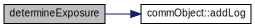
\includegraphics[width=327pt]{main_8cpp_a0416912fce6274568e80019b10ba294f_cgraph}
\end{center}
\end{figure}
Here is the caller graph for this function\+:\nopagebreak
\begin{figure}[H]
\begin{center}
\leavevmode
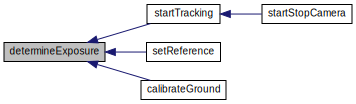
\includegraphics[width=350pt]{main_8cpp_a0416912fce6274568e80019b10ba294f_icgraph}
\end{center}
\end{figure}
\mbox{\Hypertarget{main_8cpp_a11ff459289305229597defd39f510959}\label{main_8cpp_a11ff459289305229597defd39f510959}} 
\index{main.\+cpp@{main.\+cpp}!determine\+Order@{determine\+Order}}
\index{determine\+Order@{determine\+Order}!main.\+cpp@{main.\+cpp}}
\subsubsection{\texorpdfstring{determine\+Order()}{determineOrder()}}
{\footnotesize\ttfamily void determine\+Order (\begin{DoxyParamCaption}{ }\end{DoxyParamCaption})}

Compute the order of the marker points in 2D so they are the same as in the 3D array. Hence marker 1 must be in first place for both, list\+\_\+points2d and list\+\_\+points3d. 

Definition at line 1493 of file main.\+cpp.


\begin{DoxyCode}
1494 \{\textcolor{comment}{}
1495 \textcolor{comment}{    //! determine the 3D-2D correspondences that are crucial for the PnP algorithm}
1496 \textcolor{comment}{    //! Try every possible correspondence and solve PnP}
1497 \textcolor{comment}{    //! Then project the 3D marker points into the 2D camera image and check the difference }
1498 \textcolor{comment}{    //! between projected points and points as seen by the camera}
1499 \textcolor{comment}{    //! the corresponce with the smallest difference is probably the correct one}
1500 \textcolor{comment}{}\textcolor{comment}{}
1501 \textcolor{comment}{        //! the difference between true 2D points and projected points is super big}
1502 \textcolor{comment}{}    \hyperlink{main_8cpp_ab826a7ca5876afdd6c0bccf04b73b30b}{minPointDistance} = 5000;
1503     std::sort(\hyperlink{main_8cpp_ac06fee052099b9fc9f0826315bb64a4a}{pointOrderIndices}, \hyperlink{main_8cpp_ac06fee052099b9fc9f0826315bb64a4a}{pointOrderIndices} + 4);
1504 \textcolor{comment}{}
1505 \textcolor{comment}{    //! now try every possible permutation of correspondence}
1506 \textcolor{comment}{}    \textcolor{keywordflow}{do} \{\textcolor{comment}{}
1507 \textcolor{comment}{        //! reset the starting values for solvePnP}
1508 \textcolor{comment}{}        \hyperlink{main_8cpp_ae095f10a005e68d20233dc15b4077ca6}{Rvec} = \hyperlink{main_8cpp_ae101daeaec726e27690c862b7edea825}{RvecOriginal};
1509         \hyperlink{main_8cpp_a9215ba881de0242c883e5b065d6d2ff9}{Tvec} = \hyperlink{main_8cpp_a043bf1deaf5d42d47e0cce8982c1f18b}{TvecOriginal};
1510 \textcolor{comment}{}
1511 \textcolor{comment}{        //! sort the 2d points with the current permutation}
1512 \textcolor{comment}{}        \textcolor{keywordflow}{for} (\textcolor{keywordtype}{int} m = 0; m < \hyperlink{main_8cpp_ae1d37a43f631aefe76b6e540da786064}{numberMarkers}; m++)
1513         \{
1514             \hyperlink{main_8cpp_ad583e75f176dafdb7de3f214673851de}{list\_points2d}[m] = \hyperlink{main_8cpp_a54cb682bd037283c18b5a9a447ff5e5e}{list\_points2dUnsorted}[
      \hyperlink{main_8cpp_ac06fee052099b9fc9f0826315bb64a4a}{pointOrderIndices}[m]];
1515         \}
1516 \textcolor{comment}{}
1517 \textcolor{comment}{        //! Call solve PNP with P3P since its more robust and sufficient for start value determination}
1518 \textcolor{comment}{}        solvePnP(\hyperlink{main_8cpp_a933edb4ba1c0589d59020164c2f1ff87}{list\_points3d}, \hyperlink{main_8cpp_ad583e75f176dafdb7de3f214673851de}{list\_points2d}, 
      \hyperlink{main_8cpp_a53e8957a459b639ca82d938157f3b085}{cameraMatrix}, \hyperlink{main_8cpp_a8d67876da148be9118bba1c0d017fb57}{distCoeffs}, \hyperlink{main_8cpp_ae095f10a005e68d20233dc15b4077ca6}{Rvec}, \hyperlink{main_8cpp_a9215ba881de0242c883e5b065d6d2ff9}{Tvec}, \hyperlink{main_8cpp_ab1cc9be1ff0871bc5de1eb4c2811ae3e}{useGuess}, SOLVEPNP\_P3P);
1519 \textcolor{comment}{}
1520 \textcolor{comment}{        //! set the current difference of all point correspondences to zero}
1521 \textcolor{comment}{}        \hyperlink{main_8cpp_afe37bd67ad83a2d897cf5977cba70ef3}{currentPointDistance} = 0;
1522 \textcolor{comment}{}
1523 \textcolor{comment}{        //! project the 3D points with the solvePnP solution onto 2D}
1524 \textcolor{comment}{}        projectPoints(\hyperlink{main_8cpp_a933edb4ba1c0589d59020164c2f1ff87}{list\_points3d}, \hyperlink{main_8cpp_ae095f10a005e68d20233dc15b4077ca6}{Rvec}, \hyperlink{main_8cpp_a9215ba881de0242c883e5b065d6d2ff9}{Tvec}, 
      \hyperlink{main_8cpp_a53e8957a459b639ca82d938157f3b085}{cameraMatrix}, \hyperlink{main_8cpp_a8d67876da148be9118bba1c0d017fb57}{distCoeffs}, \hyperlink{main_8cpp_a7b88d0425a68875639d40a17079df819}{list\_points2dProjected});
1525 \textcolor{comment}{}
1526 \textcolor{comment}{        //! now compute the absolute difference (error)}
1527 \textcolor{comment}{}        \textcolor{keywordflow}{for} (\textcolor{keywordtype}{int} n = 0; n < \hyperlink{main_8cpp_ae1d37a43f631aefe76b6e540da786064}{numberMarkers}; n++)
1528         \{
1529             \hyperlink{main_8cpp_afe37bd67ad83a2d897cf5977cba70ef3}{currentPointDistance} += norm(\hyperlink{main_8cpp_ad583e75f176dafdb7de3f214673851de}{list\_points2d}[n] - 
      \hyperlink{main_8cpp_a7b88d0425a68875639d40a17079df819}{list\_points2dProjected}[n]);
1530         \}
1531 \textcolor{comment}{}
1532 \textcolor{comment}{        //! if the difference with the current permutation is smaller than the smallest value till now}
1533 \textcolor{comment}{        //! it is probably the more correct permutation}
1534 \textcolor{comment}{}        \textcolor{keywordflow}{if} (\hyperlink{main_8cpp_afe37bd67ad83a2d897cf5977cba70ef3}{currentPointDistance} < \hyperlink{main_8cpp_ab826a7ca5876afdd6c0bccf04b73b30b}{minPointDistance})
1535         \{
1536             \hyperlink{main_8cpp_ab826a7ca5876afdd6c0bccf04b73b30b}{minPointDistance} = \hyperlink{main_8cpp_afe37bd67ad83a2d897cf5977cba70ef3}{currentPointDistance};    \textcolor{comment}{//!< set the
       smallest value of difference to the current one}
1537 \textcolor{comment}{}            \textcolor{keywordflow}{for} (\textcolor{keywordtype}{int} b = 0; b < \hyperlink{main_8cpp_ae1d37a43f631aefe76b6e540da786064}{numberMarkers}; b++)    \textcolor{comment}{//!< now safe the better permutation}
1538 \textcolor{comment}{}            \{
1539                 \hyperlink{main_8cpp_acc9e758efd664582db86f976cec195fa}{pointOrderIndicesNew}[b] = \hyperlink{main_8cpp_ac06fee052099b9fc9f0826315bb64a4a}{pointOrderIndices}[b];
1540             \}
1541         \}
1542 
1543 
1544     \}\textcolor{comment}{}
1545 \textcolor{comment}{    //! try every permutation }
1546 \textcolor{comment}{}    \textcolor{keywordflow}{while} (std::next\_permutation(\hyperlink{main_8cpp_ac06fee052099b9fc9f0826315bb64a4a}{pointOrderIndices}, 
      \hyperlink{main_8cpp_ac06fee052099b9fc9f0826315bb64a4a}{pointOrderIndices} + 4));
1547 \textcolor{comment}{}
1548 \textcolor{comment}{    //! now that the correct order is found assign it to the indices array}
1549 \textcolor{comment}{}    \textcolor{keywordflow}{for} (\textcolor{keywordtype}{int} w = 0; w < \hyperlink{main_8cpp_ae1d37a43f631aefe76b6e540da786064}{numberMarkers}; w++)
1550     \{
1551         \hyperlink{main_8cpp_ac06fee052099b9fc9f0826315bb64a4a}{pointOrderIndices}[w] = \hyperlink{main_8cpp_acc9e758efd664582db86f976cec195fa}{pointOrderIndicesNew}[w];
1552     \}
1553     \hyperlink{main_8cpp_acf655f393e3996144226399a338e8d3b}{gotOrder} = \textcolor{keyword}{true};
1554 \}
\end{DoxyCode}
Here is the caller graph for this function\+:\nopagebreak
\begin{figure}[H]
\begin{center}
\leavevmode
\includegraphics[width=350pt]{main_8cpp_a11ff459289305229597defd39f510959_icgraph}
\end{center}
\end{figure}
\mbox{\Hypertarget{main_8cpp_af6430ad2592a955a3618549547dfc5be}\label{main_8cpp_af6430ad2592a955a3618549547dfc5be}} 
\index{main.\+cpp@{main.\+cpp}!draw\+Position\+Text@{draw\+Position\+Text}}
\index{draw\+Position\+Text@{draw\+Position\+Text}!main.\+cpp@{main.\+cpp}}
\subsubsection{\texorpdfstring{draw\+Position\+Text()}{drawPositionText()}}
{\footnotesize\ttfamily void draw\+Position\+Text (\begin{DoxyParamCaption}\item[{cv\+::\+Mat \&}]{Picture,  }\item[{cv\+::\+Vec3d \&}]{Position,  }\item[{cv\+::\+Vec3d \&}]{Euler,  }\item[{double}]{error }\end{DoxyParamCaption})}

Draw the position, attitude and reprojection error in the picture. 
\begin{DoxyParams}[1]{Parameters}
\mbox{\tt in}  & {\em Picture} & is the camera image in Open\+CV matrix format. \\
\hline
\mbox{\tt in}  & {\em Position} & is the position of the tracked object in navigation Co\+Sy. \\
\hline
\mbox{\tt in}  & {\em Euler} & are the Euler angles with respect to the navigation frame. \\
\hline
\mbox{\tt in}  & {\em error} & is the reprojection error of the pose estimation. \\
\hline
\end{DoxyParams}


Definition at line 1310 of file main.\+cpp.


\begin{DoxyCode}
1311 \{
1312     \hyperlink{main_8cpp_a8fc3524f4e679a41dcc8d0f302d637ed}{ss}.str(\textcolor{stringliteral}{""});
1313     \hyperlink{main_8cpp_a8fc3524f4e679a41dcc8d0f302d637ed}{ss} << \textcolor{stringliteral}{"X: "} << Position[0] << \textcolor{stringliteral}{" m"};
1314     putText(Picture, \hyperlink{main_8cpp_a8fc3524f4e679a41dcc8d0f302d637ed}{ss}.str(), cv::Point(200, 440), 1, 1, cv::Scalar(255, 255, 255));
1315 
1316     \hyperlink{main_8cpp_a8fc3524f4e679a41dcc8d0f302d637ed}{ss}.str(\textcolor{stringliteral}{""});
1317     \hyperlink{main_8cpp_a8fc3524f4e679a41dcc8d0f302d637ed}{ss} << \textcolor{stringliteral}{"Y: "} << Position[1] << \textcolor{stringliteral}{" m"};
1318     putText(Picture, \hyperlink{main_8cpp_a8fc3524f4e679a41dcc8d0f302d637ed}{ss}.str(), cv::Point(200, 455), 1, 1, cv::Scalar(255, 255, 255));
1319 
1320     \hyperlink{main_8cpp_a8fc3524f4e679a41dcc8d0f302d637ed}{ss}.str(\textcolor{stringliteral}{""});
1321     \hyperlink{main_8cpp_a8fc3524f4e679a41dcc8d0f302d637ed}{ss} << \textcolor{stringliteral}{"Z: "} << Position[2] << \textcolor{stringliteral}{" m"};
1322     putText(Picture, \hyperlink{main_8cpp_a8fc3524f4e679a41dcc8d0f302d637ed}{ss}.str(), cv::Point(200, 470), 1, 1, cv::Scalar(255, 255, 255));
1323 
1324     \hyperlink{main_8cpp_a8fc3524f4e679a41dcc8d0f302d637ed}{ss}.str(\textcolor{stringliteral}{""});
1325     \hyperlink{main_8cpp_a8fc3524f4e679a41dcc8d0f302d637ed}{ss} << \textcolor{stringliteral}{"Heading: "} << Euler[2] << \textcolor{stringliteral}{" deg"};
1326     putText(Picture, \hyperlink{main_8cpp_a8fc3524f4e679a41dcc8d0f302d637ed}{ss}.str(), cv::Point(350, 440), 1, 1, cv::Scalar(255, 255, 255));
1327 
1328     \hyperlink{main_8cpp_a8fc3524f4e679a41dcc8d0f302d637ed}{ss}.str(\textcolor{stringliteral}{""});
1329     \hyperlink{main_8cpp_a8fc3524f4e679a41dcc8d0f302d637ed}{ss} << \textcolor{stringliteral}{"Pitch: "} << Euler[1] << \textcolor{stringliteral}{" deg"};
1330     putText(Picture, \hyperlink{main_8cpp_a8fc3524f4e679a41dcc8d0f302d637ed}{ss}.str(), cv::Point(350, 455), 1, 1, cv::Scalar(255, 255, 255));
1331 
1332     \hyperlink{main_8cpp_a8fc3524f4e679a41dcc8d0f302d637ed}{ss}.str(\textcolor{stringliteral}{""});
1333     \hyperlink{main_8cpp_a8fc3524f4e679a41dcc8d0f302d637ed}{ss} << \textcolor{stringliteral}{"Roll: "} << Euler[0] << \textcolor{stringliteral}{" deg"};
1334     putText(Picture, \hyperlink{main_8cpp_a8fc3524f4e679a41dcc8d0f302d637ed}{ss}.str(), cv::Point(350, 470), 1, 1, cv::Scalar(255, 255, 255));
1335 
1336     \hyperlink{main_8cpp_a8fc3524f4e679a41dcc8d0f302d637ed}{ss}.str(\textcolor{stringliteral}{""});
1337     \hyperlink{main_8cpp_a8fc3524f4e679a41dcc8d0f302d637ed}{ss} << \textcolor{stringliteral}{"Error: "} << error << \textcolor{stringliteral}{" px"};
1338     putText(Picture, \hyperlink{main_8cpp_a8fc3524f4e679a41dcc8d0f302d637ed}{ss}.str(), cv::Point(10, 470), 1, 1, cv::Scalar(255, 255, 255));
1339 \}
\end{DoxyCode}
Here is the caller graph for this function\+:\nopagebreak
\begin{figure}[H]
\begin{center}
\leavevmode
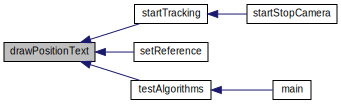
\includegraphics[width=350pt]{main_8cpp_af6430ad2592a955a3618549547dfc5be_icgraph}
\end{center}
\end{figure}
\mbox{\Hypertarget{main_8cpp_ab2b71933055cf32cc8e5e2100fd7723f}\label{main_8cpp_ab2b71933055cf32cc8e5e2100fd7723f}} 
\index{main.\+cpp@{main.\+cpp}!get\+Euler\+Angles@{get\+Euler\+Angles}}
\index{get\+Euler\+Angles@{get\+Euler\+Angles}!main.\+cpp@{main.\+cpp}}
\subsubsection{\texorpdfstring{get\+Euler\+Angles()}{getEulerAngles()}}
{\footnotesize\ttfamily void get\+Euler\+Angles (\begin{DoxyParamCaption}\item[{Mat \&}]{rot\+Camer\+Matrix,  }\item[{Vec3d \&}]{euler\+Angles }\end{DoxyParamCaption})}

Get the euler angles from a rotation matrix 
\begin{DoxyParams}[1]{Parameters}
\mbox{\tt in}  & {\em rot\+Camer\+Matrix} & is a projection matrix, here normally only the extrinsic values. \\
\hline
\mbox{\tt out}  & {\em euler\+Angles} & contains the Euler angles that result in the same rotation matrix as rot\+Camer\+Matrix. \\
\hline
\end{DoxyParams}


Definition at line 236 of file main.\+cpp.


\begin{DoxyCode}
236                                                              \{
237 
238     Mat \hyperlink{main_8cpp_a53e8957a459b639ca82d938157f3b085}{cameraMatrix}, rotMatrix, transVect, rotMatrixX, rotMatrixY, rotMatrixZ;
239     \textcolor{keywordtype}{double}* \_r = rotCamerMatrix.ptr<\textcolor{keywordtype}{double}>();
240     \textcolor{keywordtype}{double} projMatrix[12] = \{ \_r[0],\_r[1],\_r[2],0,
241         \_r[3],\_r[4],\_r[5],0,
242         \_r[6],\_r[7],\_r[8],0 \};
243 
244     decomposeProjectionMatrix(Mat(3, 4, CV\_64FC1, projMatrix),
245         cameraMatrix,
246         rotMatrix,
247         transVect,
248         rotMatrixX,
249         rotMatrixY,
250         rotMatrixZ,
251         \hyperlink{main_8cpp_a0a53d01e06c71d6360afcb0fabf2aa8e}{eulerAngles});
252 \}
\end{DoxyCode}
Here is the caller graph for this function\+:\nopagebreak
\begin{figure}[H]
\begin{center}
\leavevmode
\includegraphics[width=350pt]{main_8cpp_ab2b71933055cf32cc8e5e2100fd7723f_icgraph}
\end{center}
\end{figure}
\mbox{\Hypertarget{main_8cpp_ad39626702ff983d5fdab4b703bfaf964}\label{main_8cpp_ad39626702ff983d5fdab4b703bfaf964}} 
\index{main.\+cpp@{main.\+cpp}!load\+Calibration@{load\+Calibration}}
\index{load\+Calibration@{load\+Calibration}!main.\+cpp@{main.\+cpp}}
\subsubsection{\texorpdfstring{load\+Calibration()}{loadCalibration()}}
{\footnotesize\ttfamily void load\+Calibration (\begin{DoxyParamCaption}\item[{int}]{method }\end{DoxyParamCaption})}

Load a previously saved camera calibration from a file. 
\begin{DoxyParams}[1]{Parameters}
\mbox{\tt in}  & {\em method} & whether or not load the camera calibration from calibration.\+xml. If ==0 then yes, if != 0 then let the user select a different file. \\
\hline
\end{DoxyParams}


Definition at line 918 of file main.\+cpp.


\begin{DoxyCode}
918                                  \{
919 
920     QString fileName;
921     \textcolor{keywordflow}{if} (method == 0)
922     \{
923         fileName = \textcolor{stringliteral}{"calibration.xml"};
924     \}
925     \textcolor{keywordflow}{else}
926     \{
927         fileName = QFileDialog::getOpenFileName(\textcolor{keyword}{nullptr}, \textcolor{stringliteral}{"Choose a previous saved calibration file"}, \textcolor{stringliteral}{""}, \textcolor{stringliteral}{"
      Calibration Files (*.xml);;All Files (*)"});
928         \textcolor{keywordflow}{if} (fileName.length() == 0)
929         \{
930             fileName = \textcolor{stringliteral}{"calibration.xml"};
931         \}
932     \}
933     FileStorage fs;
934     fs.open(fileName.toUtf8().constData(), FileStorage::READ);
935     fs[\textcolor{stringliteral}{"CameraMatrix"}] >> \hyperlink{main_8cpp_a53e8957a459b639ca82d938157f3b085}{cameraMatrix};
936     fs[\textcolor{stringliteral}{"DistCoeff"}] >> \hyperlink{main_8cpp_a8d67876da148be9118bba1c0d017fb57}{distCoeffs};
937     \hyperlink{main_8cpp_af29e7fc07ae0979d5fb61b473241d33d}{commObj}.\hyperlink{classcomm_object_aec354c7099b3039083cc4224e071e022}{addLog}(\textcolor{stringliteral}{"Loaded calibration from file:"});
938     \hyperlink{main_8cpp_af29e7fc07ae0979d5fb61b473241d33d}{commObj}.\hyperlink{classcomm_object_aec354c7099b3039083cc4224e071e022}{addLog}(fileName);
939     \hyperlink{main_8cpp_a8fc3524f4e679a41dcc8d0f302d637ed}{ss}.str(\textcolor{stringliteral}{""});
940     \hyperlink{main_8cpp_a8fc3524f4e679a41dcc8d0f302d637ed}{ss} << \textcolor{stringliteral}{"\(\backslash\)nCamera Matrix is"} << \textcolor{stringliteral}{"\(\backslash\)n"} << cameraMatrix << \textcolor{stringliteral}{"\(\backslash\)n"};
941     \hyperlink{main_8cpp_a8fc3524f4e679a41dcc8d0f302d637ed}{ss} << \textcolor{stringliteral}{"\(\backslash\)nDistortion Coefficients are"} << \textcolor{stringliteral}{"\(\backslash\)n"} << distCoeffs << \textcolor{stringliteral}{"\(\backslash\)n"};
942     \hyperlink{main_8cpp_af29e7fc07ae0979d5fb61b473241d33d}{commObj}.\hyperlink{classcomm_object_aec354c7099b3039083cc4224e071e022}{addLog}(QString::fromStdString(\hyperlink{main_8cpp_a8fc3524f4e679a41dcc8d0f302d637ed}{ss}.str()));
943 \}
\end{DoxyCode}
Here is the call graph for this function\+:\nopagebreak
\begin{figure}[H]
\begin{center}
\leavevmode
\includegraphics[width=306pt]{main_8cpp_ad39626702ff983d5fdab4b703bfaf964_cgraph}
\end{center}
\end{figure}
Here is the caller graph for this function\+:\nopagebreak
\begin{figure}[H]
\begin{center}
\leavevmode
\includegraphics[width=350pt]{main_8cpp_ad39626702ff983d5fdab4b703bfaf964_icgraph}
\end{center}
\end{figure}
\mbox{\Hypertarget{main_8cpp_af39fa6c3a36ad6bc24a327db7a9d73c2}\label{main_8cpp_af39fa6c3a36ad6bc24a327db7a9d73c2}} 
\index{main.\+cpp@{main.\+cpp}!load\+Camera\+Position@{load\+Camera\+Position}}
\index{load\+Camera\+Position@{load\+Camera\+Position}!main.\+cpp@{main.\+cpp}}
\subsubsection{\texorpdfstring{load\+Camera\+Position()}{loadCameraPosition()}}
{\footnotesize\ttfamily void load\+Camera\+Position (\begin{DoxyParamCaption}{ }\end{DoxyParamCaption})}

Load the rotation matrix from camera Co\+Sy to ground Co\+Sy It is determined during \hyperlink{main_8cpp_a7ad2e3cfb5056dbab2098e0dd3bd353f}{calibrate\+Ground()} and stays the same once the camera is mounted and fixed. 

Definition at line 1343 of file main.\+cpp.


\begin{DoxyCode}
1344 \{\textcolor{comment}{}
1345 \textcolor{comment}{    //! Open the referenceData.xml that contains the rotation from camera CoSy to ground CoSy}
1346 \textcolor{comment}{}    FileStorage fs;
1347     fs.open(\textcolor{stringliteral}{"referenceData.xml"}, FileStorage::READ);
1348     fs[\textcolor{stringliteral}{"M\_NC"}] >> \hyperlink{main_8cpp_af604b9538ec8923428a78439eaf55f8e}{M\_CN};
1349     fs[\textcolor{stringliteral}{"M\_NC"}] >> \hyperlink{main_8cpp_a4ee4d2abbe47b92c21b81c5c4389086e}{RmatRef};
1350     fs[\textcolor{stringliteral}{"posRef"}] >> \hyperlink{main_8cpp_a9d2e25dbfda0ebcdbb488652c8b15fad}{posRef};
1351     fs[\textcolor{stringliteral}{"eulerRef"}] >> \hyperlink{main_8cpp_acd6966c004a57c4080ba204152200e7f}{eulerRef};
1352     \hyperlink{main_8cpp_af29e7fc07ae0979d5fb61b473241d33d}{commObj}.\hyperlink{classcomm_object_aec354c7099b3039083cc4224e071e022}{addLog}(\textcolor{stringliteral}{"Loaded reference pose."});
1353 \}
\end{DoxyCode}
Here is the call graph for this function\+:\nopagebreak
\begin{figure}[H]
\begin{center}
\leavevmode
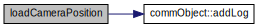
\includegraphics[width=330pt]{main_8cpp_af39fa6c3a36ad6bc24a327db7a9d73c2_cgraph}
\end{center}
\end{figure}
Here is the caller graph for this function\+:\nopagebreak
\begin{figure}[H]
\begin{center}
\leavevmode
\includegraphics[width=350pt]{main_8cpp_af39fa6c3a36ad6bc24a327db7a9d73c2_icgraph}
\end{center}
\end{figure}
\mbox{\Hypertarget{main_8cpp_a56c7f641859cb2b6b99b0947d03be800}\label{main_8cpp_a56c7f641859cb2b6b99b0947d03be800}} 
\index{main.\+cpp@{main.\+cpp}!load\+Marker\+Config@{load\+Marker\+Config}}
\index{load\+Marker\+Config@{load\+Marker\+Config}!main.\+cpp@{main.\+cpp}}
\subsubsection{\texorpdfstring{load\+Marker\+Config()}{loadMarkerConfig()}}
{\footnotesize\ttfamily void load\+Marker\+Config (\begin{DoxyParamCaption}\item[{int}]{method }\end{DoxyParamCaption})}

Load a marker configuration from file. This file has to be created by hand, use the standard marker configuration file as template. 
\begin{DoxyParams}[1]{Parameters}
\mbox{\tt in}  & {\em method} & whether or not load the configuration from the marker\+Standard.\+xml. If ==0 load it, if != 0 let the user select a different file. \\
\hline
\end{DoxyParams}


Definition at line 1190 of file main.\+cpp.


\begin{DoxyCode}
1191 \{
1192     QString fileName;\textcolor{comment}{}
1193 \textcolor{comment}{    //! during start up of the programm load the standard marker configuration}
1194 \textcolor{comment}{}    \textcolor{keywordflow}{if} (method == 0)
1195     \{\textcolor{comment}{}
1196 \textcolor{comment}{        //! open the standard marker configuration file}
1197 \textcolor{comment}{}        FileStorage fs;
1198         fs.open(\textcolor{stringliteral}{"markerStandard.xml"}, FileStorage::READ);
1199 \textcolor{comment}{}
1200 \textcolor{comment}{        //! copy the values to the respective variables}
1201 \textcolor{comment}{}        fs[\textcolor{stringliteral}{"numberMarkers"}] >> \hyperlink{main_8cpp_ae1d37a43f631aefe76b6e540da786064}{numberMarkers};
1202 \textcolor{comment}{}
1203 \textcolor{comment}{        //! inizialise vectors with correct length depending on the number of markers}
1204 \textcolor{comment}{}        \hyperlink{main_8cpp_a933edb4ba1c0589d59020164c2f1ff87}{list\_points3d} = std::vector<Point3d>(\hyperlink{main_8cpp_ae1d37a43f631aefe76b6e540da786064}{numberMarkers});
1205         \hyperlink{main_8cpp_ad583e75f176dafdb7de3f214673851de}{list\_points2d} = std::vector<Point2d>(\hyperlink{main_8cpp_ae1d37a43f631aefe76b6e540da786064}{numberMarkers});
1206         \hyperlink{main_8cpp_a85d3d8c8a0e3e9cfb6157c247470d934}{list\_points2dOld} = std::vector<Point2d>(\hyperlink{main_8cpp_ae1d37a43f631aefe76b6e540da786064}{numberMarkers});
1207         \hyperlink{main_8cpp_aea88a68a83d84419dd1c5a93b21b1958}{list\_points2dDifference} = std::vector<double>(
      \hyperlink{main_8cpp_ae1d37a43f631aefe76b6e540da786064}{numberMarkers});
1208         \hyperlink{main_8cpp_a7b88d0425a68875639d40a17079df819}{list\_points2dProjected} = std::vector<Point2d>(
      \hyperlink{main_8cpp_ae1d37a43f631aefe76b6e540da786064}{numberMarkers});
1209         \hyperlink{main_8cpp_a54cb682bd037283c18b5a9a447ff5e5e}{list\_points2dUnsorted} = std::vector<Point2d>(
      \hyperlink{main_8cpp_ae1d37a43f631aefe76b6e540da786064}{numberMarkers});
1210 \textcolor{comment}{}
1211 \textcolor{comment}{        //! save the marker locations in the points3d vector}
1212 \textcolor{comment}{}        fs[\textcolor{stringliteral}{"list\_points3d"}] >> \hyperlink{main_8cpp_a933edb4ba1c0589d59020164c2f1ff87}{list\_points3d};
1213         fs.release();
1214         \hyperlink{main_8cpp_af29e7fc07ae0979d5fb61b473241d33d}{commObj}.\hyperlink{classcomm_object_aec354c7099b3039083cc4224e071e022}{addLog}(\textcolor{stringliteral}{"Loaded marker configuration from file:"});
1215         \hyperlink{main_8cpp_af29e7fc07ae0979d5fb61b473241d33d}{commObj}.\hyperlink{classcomm_object_aec354c7099b3039083cc4224e071e022}{addLog}(fileName);
1216 
1217 
1218 
1219     \}
1220     \textcolor{keywordflow}{else}
1221     \{\textcolor{comment}{}
1222 \textcolor{comment}{        //! if the load marker configuration button was clicked show a open file dialog }
1223 \textcolor{comment}{}        fileName = QFileDialog::getOpenFileName(\textcolor{keyword}{nullptr}, \textcolor{stringliteral}{"Choose a previous saved marker configuration file
      "}, \textcolor{stringliteral}{""}, \textcolor{stringliteral}{"marker configuratio files (*.xml);;All Files (*)"});
1224 \textcolor{comment}{}
1225 \textcolor{comment}{        //! was cancel or abort clicked }
1226 \textcolor{comment}{}        \textcolor{keywordflow}{if} (fileName.length() == 0)
1227         \{\textcolor{comment}{}
1228 \textcolor{comment}{            //! if yes load the standard marker configuration}
1229 \textcolor{comment}{}            fileName = \textcolor{stringliteral}{"markerStandard.xml"};
1230         \}
1231 \textcolor{comment}{}
1232 \textcolor{comment}{        //! open the selected marker configuration file}
1233 \textcolor{comment}{}        FileStorage fs;
1234         fs.open(fileName.toUtf8().constData(), FileStorage::READ);
1235 \textcolor{comment}{}
1236 \textcolor{comment}{        //! copy the values to the respective variables}
1237 \textcolor{comment}{}        fs[\textcolor{stringliteral}{"numberMarkers"}] >> \hyperlink{main_8cpp_ae1d37a43f631aefe76b6e540da786064}{numberMarkers};
1238 \textcolor{comment}{}
1239 \textcolor{comment}{        //! inizialise vectors with correct length depending on the number of markers}
1240 \textcolor{comment}{}        list\_points3d = std::vector<Point3d>(\hyperlink{main_8cpp_ae1d37a43f631aefe76b6e540da786064}{numberMarkers});
1241         list\_points2d = std::vector<Point2d>(\hyperlink{main_8cpp_ae1d37a43f631aefe76b6e540da786064}{numberMarkers});
1242         list\_points2dOld = std::vector<Point2d>(\hyperlink{main_8cpp_ae1d37a43f631aefe76b6e540da786064}{numberMarkers});
1243         list\_points2dDifference = std::vector<double>(\hyperlink{main_8cpp_ae1d37a43f631aefe76b6e540da786064}{numberMarkers});
1244         list\_points2dProjected = std::vector<Point2d>(\hyperlink{main_8cpp_ae1d37a43f631aefe76b6e540da786064}{numberMarkers});
1245         list\_points2dUnsorted = std::vector<Point2d>(\hyperlink{main_8cpp_ae1d37a43f631aefe76b6e540da786064}{numberMarkers});
1246 \textcolor{comment}{}
1247 \textcolor{comment}{        //! save the marker locations in the points3d vector}
1248 \textcolor{comment}{}        fs[\textcolor{stringliteral}{"list\_points3d"}] >> \hyperlink{main_8cpp_a933edb4ba1c0589d59020164c2f1ff87}{list\_points3d};
1249         fs.release();
1250         \hyperlink{main_8cpp_af29e7fc07ae0979d5fb61b473241d33d}{commObj}.\hyperlink{classcomm_object_aec354c7099b3039083cc4224e071e022}{addLog}(\textcolor{stringliteral}{"Loaded marker configuration from file:"});
1251         \hyperlink{main_8cpp_af29e7fc07ae0979d5fb61b473241d33d}{commObj}.\hyperlink{classcomm_object_aec354c7099b3039083cc4224e071e022}{addLog}(fileName);
1252 
1253     \}
1254 \textcolor{comment}{}
1255 \textcolor{comment}{    //! Print out the number of markers and their position to the GUI}
1256 \textcolor{comment}{}    \hyperlink{main_8cpp_a8fc3524f4e679a41dcc8d0f302d637ed}{ss}.str(\textcolor{stringliteral}{""});
1257     \hyperlink{main_8cpp_a8fc3524f4e679a41dcc8d0f302d637ed}{ss} << \textcolor{stringliteral}{"Number of Markers: "} << numberMarkers << \textcolor{stringliteral}{"\(\backslash\)n"};
1258     \hyperlink{main_8cpp_a8fc3524f4e679a41dcc8d0f302d637ed}{ss} << \textcolor{stringliteral}{"Marker 3D Points X,Y and Z [mm]: \(\backslash\)n"};
1259     \textcolor{keywordflow}{for} (\textcolor{keywordtype}{int} i = 0; i < \hyperlink{main_8cpp_ae1d37a43f631aefe76b6e540da786064}{numberMarkers}; i++)
1260     \{
1261         \hyperlink{main_8cpp_a8fc3524f4e679a41dcc8d0f302d637ed}{ss} << \textcolor{stringliteral}{"Marker "} << i + 1 << \textcolor{stringliteral}{":\(\backslash\)t"} << list\_points3d[i].x << \textcolor{stringliteral}{"\(\backslash\)t"} << list\_points3d[i].y << \textcolor{stringliteral}{"\(\backslash\)t"} << 
      list\_points3d[i].z << \textcolor{stringliteral}{"\(\backslash\)n"};
1262     \}
1263     \hyperlink{main_8cpp_af29e7fc07ae0979d5fb61b473241d33d}{commObj}.\hyperlink{classcomm_object_aec354c7099b3039083cc4224e071e022}{addLog}(QString::fromStdString(\hyperlink{main_8cpp_a8fc3524f4e679a41dcc8d0f302d637ed}{ss}.str()));
1264 \textcolor{comment}{}
1265 \textcolor{comment}{    //! check if P3P algorithm can be enabled, it needs exactly 4 marker points to work}
1266 \textcolor{comment}{}    \textcolor{keywordflow}{if} (numberMarkers == 4)
1267     \{\textcolor{comment}{}
1268 \textcolor{comment}{        //! if P3P is possible, let the user choose which algorithm he wants but keep iterative active}
1269 \textcolor{comment}{}        \hyperlink{main_8cpp_ab5e634b66221f494504aea1557af5df9}{methodPNP} = 0;
1270         \hyperlink{main_8cpp_af29e7fc07ae0979d5fb61b473241d33d}{commObj}.\hyperlink{classcomm_object_a7552116eb5e18c49c6dcf943de29af7a}{enableP3P}(\textcolor{keyword}{true});
1271     \}
1272     \textcolor{keywordflow}{else}
1273     \{\textcolor{comment}{}
1274 \textcolor{comment}{        //! More (or less) marker than 4 loaded, P3P is not possible, hence user cant select P3P in GUI}
1275 \textcolor{comment}{}        \hyperlink{main_8cpp_ab5e634b66221f494504aea1557af5df9}{methodPNP} = 0;
1276         \hyperlink{main_8cpp_af29e7fc07ae0979d5fb61b473241d33d}{commObj}.\hyperlink{classcomm_object_a7552116eb5e18c49c6dcf943de29af7a}{enableP3P}(\textcolor{keyword}{false});
1277         \hyperlink{main_8cpp_af29e7fc07ae0979d5fb61b473241d33d}{commObj}.\hyperlink{classcomm_object_aec354c7099b3039083cc4224e071e022}{addLog}(\textcolor{stringliteral}{"P3P algorithm disabled, only works with 4 markers."});
1278     \}
1279 \textcolor{comment}{}
1280 \textcolor{comment}{    //! now display the marker configuration in the camera view }
1281 \textcolor{comment}{}    Mat cFrame(480, 640, CV\_8UC3, Scalar(0, 0, 0));
1282 \textcolor{comment}{}
1283 \textcolor{comment}{    //! Set the camera pose parallel to the marker coordinate system}
1284 \textcolor{comment}{}    \hyperlink{main_8cpp_a9215ba881de0242c883e5b065d6d2ff9}{Tvec}.at<\textcolor{keywordtype}{double}>(0) = 0;
1285     \hyperlink{main_8cpp_a9215ba881de0242c883e5b065d6d2ff9}{Tvec}.at<\textcolor{keywordtype}{double}>(1) = 0;
1286     \hyperlink{main_8cpp_a9215ba881de0242c883e5b065d6d2ff9}{Tvec}.at<\textcolor{keywordtype}{double}>(2) = 4500;
1287     \hyperlink{main_8cpp_ae095f10a005e68d20233dc15b4077ca6}{Rvec}.at<\textcolor{keywordtype}{double}>(0) = 0 * 3.141592653589 / 180.0;
1288     \hyperlink{main_8cpp_ae095f10a005e68d20233dc15b4077ca6}{Rvec}.at<\textcolor{keywordtype}{double}>(1) = 0 * 3.141592653589 / 180.0;
1289     \hyperlink{main_8cpp_ae095f10a005e68d20233dc15b4077ca6}{Rvec}.at<\textcolor{keywordtype}{double}>(2) = -90. * 3.141592653589 / 180.0;
1290 
1291     projectPoints(list\_points3d, \hyperlink{main_8cpp_ae095f10a005e68d20233dc15b4077ca6}{Rvec}, \hyperlink{main_8cpp_a9215ba881de0242c883e5b065d6d2ff9}{Tvec}, \hyperlink{main_8cpp_a53e8957a459b639ca82d938157f3b085}{cameraMatrix}, 
      \hyperlink{main_8cpp_a8d67876da148be9118bba1c0d017fb57}{distCoeffs}, list\_points2dProjected);
1292     \textcolor{keywordflow}{for} (\textcolor{keywordtype}{int} i = 0; i < \hyperlink{main_8cpp_ae1d37a43f631aefe76b6e540da786064}{numberMarkers}; i++)
1293     \{
1294         circle(cFrame, Point(list\_points2dProjected[i].x, list\_points2dProjected[i].y), 3, Scalar(255, 0, 0
      ), 3);
1295     \}
1296 
1297     \hyperlink{main_8cpp_a2104a5d9d6b9f1e29bc4cd858c59882e}{projectCoordinateFrame}(cFrame);
1298     QPixmap QPFrame;
1299     QPFrame = \hyperlink{main_8cpp_a3e3cc959a7ab6f93ea52863d86373ce5}{Mat2QPixmap}(cFrame);
1300     \hyperlink{main_8cpp_af29e7fc07ae0979d5fb61b473241d33d}{commObj}.\hyperlink{classcomm_object_a6f81522c2aa1668fa402f08710e6206b}{changeImage}(QPFrame);
1301     QCoreApplication::processEvents();
1302 
1303 \}
\end{DoxyCode}
Here is the call graph for this function\+:\nopagebreak
\begin{figure}[H]
\begin{center}
\leavevmode
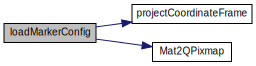
\includegraphics[width=344pt]{main_8cpp_a56c7f641859cb2b6b99b0947d03be800_cgraph}
\end{center}
\end{figure}
Here is the caller graph for this function\+:\nopagebreak
\begin{figure}[H]
\begin{center}
\leavevmode
\includegraphics[width=350pt]{main_8cpp_a56c7f641859cb2b6b99b0947d03be800_icgraph}
\end{center}
\end{figure}
\mbox{\Hypertarget{main_8cpp_a0ddf1224851353fc92bfbff6f499fa97}\label{main_8cpp_a0ddf1224851353fc92bfbff6f499fa97}} 
\index{main.\+cpp@{main.\+cpp}!main@{main}}
\index{main@{main}!main.\+cpp@{main.\+cpp}}
\subsubsection{\texorpdfstring{main()}{main()}}
{\footnotesize\ttfamily int main (\begin{DoxyParamCaption}\item[{int}]{argc,  }\item[{char $\ast$}]{argv\mbox{[}$\,$\mbox{]} }\end{DoxyParamCaption})}



main initialises the G\+UI and values for the marker position etc 

First the G\+UI is set up with Signals and Slots, see Qt docu for how that works. Then some variables are initialized with arbitrary values. At last calibration and marker configuration etc. are loaded from xml files. 
\begin{DoxyParams}[1]{Parameters}
\mbox{\tt in}  & {\em argc} & is not used. \\
\hline
\mbox{\tt in}  & {\em argv} & is also not used. \\
\hline
\end{DoxyParams}


Definition at line 151 of file main.\+cpp.


\begin{DoxyCode}
152 \{
153     QApplication a(argc, argv);
154     \hyperlink{class_rigid_track}{RigidTrack} w;
155     w.show();   \textcolor{comment}{//!< show the GUI}
156 \textcolor{comment}{}\textcolor{comment}{    //! connect the Qt slots and signals for event handling}
157 \textcolor{comment}{}    QObject::connect(&\hyperlink{main_8cpp_af29e7fc07ae0979d5fb61b473241d33d}{commObj}, SIGNAL(statusChanged(QString)), &w, SLOT(setStatus(QString)), 
      Qt::DirectConnection);
158     QObject::connect(&\hyperlink{main_8cpp_af29e7fc07ae0979d5fb61b473241d33d}{commObj}, SIGNAL(imageChanged(QPixmap)), &w, SLOT(setImage(QPixmap)), 
      Qt::DirectConnection);
159     QObject::connect(&\hyperlink{main_8cpp_af29e7fc07ae0979d5fb61b473241d33d}{commObj}, SIGNAL(logAdded(QString)), &w, SLOT(setLog(QString)), 
      Qt::DirectConnection);
160     QObject::connect(&\hyperlink{main_8cpp_af29e7fc07ae0979d5fb61b473241d33d}{commObj}, SIGNAL(logCleared()), &w, SLOT(clearLog(QString)), 
      Qt::DirectConnection);
161     QObject::connect(&\hyperlink{main_8cpp_af29e7fc07ae0979d5fb61b473241d33d}{commObj}, SIGNAL(P3Penabled(\textcolor{keywordtype}{bool})), &w, SLOT(enableP3P(\textcolor{keywordtype}{bool})), 
      Qt::DirectConnection);
162     QObject::connect(&\hyperlink{main_8cpp_af29e7fc07ae0979d5fb61b473241d33d}{commObj}, SIGNAL(progressUpdated(\textcolor{keywordtype}{int})), &w, SLOT(progressUpdate(\textcolor{keywordtype}{int})), 
      Qt::DirectConnection);
163 
164     \hyperlink{main_8cpp_af29e7fc07ae0979d5fb61b473241d33d}{commObj}.\hyperlink{classcomm_object_aec354c7099b3039083cc4224e071e022}{addLog}(\textcolor{stringliteral}{"RigidTrack Version:"});
165     \hyperlink{main_8cpp_af29e7fc07ae0979d5fb61b473241d33d}{commObj}.\hyperlink{classcomm_object_aec354c7099b3039083cc4224e071e022}{addLog}(QString::number(\_MSC\_FULL\_VER));
166     \hyperlink{main_8cpp_af29e7fc07ae0979d5fb61b473241d33d}{commObj}.\hyperlink{classcomm_object_aec354c7099b3039083cc4224e071e022}{addLog}(\textcolor{stringliteral}{"Built on:"});
167     \hyperlink{main_8cpp_af29e7fc07ae0979d5fb61b473241d33d}{commObj}.\hyperlink{classcomm_object_aec354c7099b3039083cc4224e071e022}{addLog}(QString(\_\_DATE\_\_));
168 \textcolor{comment}{}
169 \textcolor{comment}{    //! initial guesses for position and rotation, important for Iterative Method!}
170 \textcolor{comment}{}    \hyperlink{main_8cpp_a9215ba881de0242c883e5b065d6d2ff9}{Tvec}.at<\textcolor{keywordtype}{double}>(0) = 45;
171     \hyperlink{main_8cpp_a9215ba881de0242c883e5b065d6d2ff9}{Tvec}.at<\textcolor{keywordtype}{double}>(1) = 45;
172     \hyperlink{main_8cpp_a9215ba881de0242c883e5b065d6d2ff9}{Tvec}.at<\textcolor{keywordtype}{double}>(2) = 4500;
173     \hyperlink{main_8cpp_ae095f10a005e68d20233dc15b4077ca6}{Rvec}.at<\textcolor{keywordtype}{double}>(0) = 0 * 3.141592653589 / 180.0;
174     \hyperlink{main_8cpp_ae095f10a005e68d20233dc15b4077ca6}{Rvec}.at<\textcolor{keywordtype}{double}>(1) = 0 * 3.141592653589 / 180.0;
175     \hyperlink{main_8cpp_ae095f10a005e68d20233dc15b4077ca6}{Rvec}.at<\textcolor{keywordtype}{double}>(2) = -45 * 3.141592653589 / 180.0;
176 \textcolor{comment}{}
177 \textcolor{comment}{    //! Points that make up the marker CoSy axis system, hence one line in each axis direction}
178 \textcolor{comment}{}    \hyperlink{main_8cpp_ab34a04f5429de54d618fe1c9bd363c4e}{coordinateFrame} = std::vector<Point3d>(4);
179     \hyperlink{main_8cpp_a25a0b285905c7882d629b8f561425a2f}{coordinateFrameProjected} = std::vector<Point2d>(4);
180     coordinateFrame[0] = cv::Point3d(0, 0, 0);
181     coordinateFrame[1] = cv::Point3d(300, 0, 0);
182     coordinateFrame[2] = cv::Point3d(0, 300, 0);
183     coordinateFrame[3] = cv::Point3d(0, 0, 300);
184 
185     \hyperlink{main_8cpp_ac6dab448fd1f9b3aed1205fbd8179f5d}{position}[0] = 1.1234;     \textcolor{comment}{//!< set position initial values}
186 \textcolor{comment}{}    \hyperlink{main_8cpp_ac6dab448fd1f9b3aed1205fbd8179f5d}{position}[1] = 1.2345;     \textcolor{comment}{//!< set position initial values}
187 \textcolor{comment}{}    \hyperlink{main_8cpp_ac6dab448fd1f9b3aed1205fbd8179f5d}{position}[2] = 1.3456;     \textcolor{comment}{//!< set position initial values}
188 \textcolor{comment}{}
189     \hyperlink{main_8cpp_a700b8df52e2beb702d06651ed6130e73}{velocity}[0] = 0.123;    \textcolor{comment}{//!< set velocity initial values}
190 \textcolor{comment}{}    \hyperlink{main_8cpp_a700b8df52e2beb702d06651ed6130e73}{velocity}[1] = 0.234;    \textcolor{comment}{//!< set velocity initial values}
191 \textcolor{comment}{}    \hyperlink{main_8cpp_a700b8df52e2beb702d06651ed6130e73}{velocity}[2] = 0.345;    \textcolor{comment}{//!< set velocity initial values}
192 \textcolor{comment}{}
193     \hyperlink{main_8cpp_a0a53d01e06c71d6360afcb0fabf2aa8e}{eulerAngles}[0] = 1.002;  \textcolor{comment}{//!< set initial euler angles to arbitrary values for testing}
194 \textcolor{comment}{}    \hyperlink{main_8cpp_a0a53d01e06c71d6360afcb0fabf2aa8e}{eulerAngles}[1] = 1.003;  \textcolor{comment}{//!< set initial euler angles to arbitrary values for testing}
195 \textcolor{comment}{}    \hyperlink{main_8cpp_a0a53d01e06c71d6360afcb0fabf2aa8e}{eulerAngles}[2] = 1.004;  \textcolor{comment}{//!< set initial euler angles to arbitrary values for testing}
196 \textcolor{comment}{}
197     \hyperlink{main_8cpp_ad19da4e648bbdc80d3123eb94711588e}{setHeadingOffset}(0.0); \textcolor{comment}{//!< set the heading offset to 0 }
198 \textcolor{comment}{}
199     \hyperlink{main_8cpp_a8fc3524f4e679a41dcc8d0f302d637ed}{ss}.precision(4); \textcolor{comment}{//!< outputs in the log etc are limited to 3 decimal values}
200 \textcolor{comment}{}
201     \hyperlink{main_8cpp_af39fa6c3a36ad6bc24a327db7a9d73c2}{loadCameraPosition}(); \textcolor{comment}{//!< load the rotation matrix from camera CoSy to ground CoSy}
202 \textcolor{comment}{}    \hyperlink{main_8cpp_ad39626702ff983d5fdab4b703bfaf964}{loadCalibration}(0); \textcolor{comment}{//!< load the calibration file with the camera intrinsics}
203 \textcolor{comment}{}    \hyperlink{main_8cpp_a56c7f641859cb2b6b99b0947d03be800}{loadMarkerConfig}(0); \textcolor{comment}{//!< load the standard marker configuration}
204 \textcolor{comment}{}    \hyperlink{main_8cpp_a847c0fbd3e513fb76ff145b31a9f5c37}{testAlgorithms}(); \textcolor{comment}{//!< test the algorithms and their accuracy}
205 \textcolor{comment}{}
206     \textcolor{keywordflow}{return} a.exec();
207 \}
\end{DoxyCode}
Here is the call graph for this function\+:\nopagebreak
\begin{figure}[H]
\begin{center}
\leavevmode
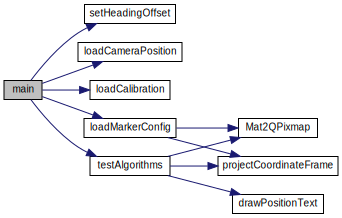
\includegraphics[width=350pt]{main_8cpp_a0ddf1224851353fc92bfbff6f499fa97_cgraph}
\end{center}
\end{figure}
Here is the caller graph for this function\+:\nopagebreak
\begin{figure}[H]
\begin{center}
\leavevmode
\includegraphics[width=350pt]{main_8cpp_a0ddf1224851353fc92bfbff6f499fa97_icgraph}
\end{center}
\end{figure}
\mbox{\Hypertarget{main_8cpp_a3e3cc959a7ab6f93ea52863d86373ce5}\label{main_8cpp_a3e3cc959a7ab6f93ea52863d86373ce5}} 
\index{main.\+cpp@{main.\+cpp}!Mat2\+Q\+Pixmap@{Mat2\+Q\+Pixmap}}
\index{Mat2\+Q\+Pixmap@{Mat2\+Q\+Pixmap}!main.\+cpp@{main.\+cpp}}
\subsubsection{\texorpdfstring{Mat2\+Q\+Pixmap()}{Mat2QPixmap()}}
{\footnotesize\ttfamily Q\+Pixmap Mat2\+Q\+Pixmap (\begin{DoxyParamCaption}\item[{cv\+::\+Mat}]{src }\end{DoxyParamCaption})}

Convert an opencv matrix that represents a picture to a Qt Pixmap object for the G\+UI. 
\begin{DoxyParams}[1]{Parameters}
\mbox{\tt in}  & {\em src} & is the camera image represented as Open\+CV matrix. \\
\hline
\end{DoxyParams}


Definition at line 211 of file main.\+cpp.


\begin{DoxyCode}
212 \{
213     QImage dest((\textcolor{keyword}{const} uchar *)src.data, src.cols, src.rows, src.step, QImage::Format\_RGB888);
214     dest.bits(); \textcolor{comment}{//! enforce deep copy, see documentation }
215 \textcolor{comment}{}\textcolor{comment}{                 //! of QImage::QImage ( const uchar * data, int width, int height, Format format )}
216 \textcolor{comment}{}    QPixmap pixmapDest = QPixmap::fromImage(dest);
217     \textcolor{keywordflow}{return} pixmapDest;
218 \}
\end{DoxyCode}
Here is the caller graph for this function\+:\nopagebreak
\begin{figure}[H]
\begin{center}
\leavevmode
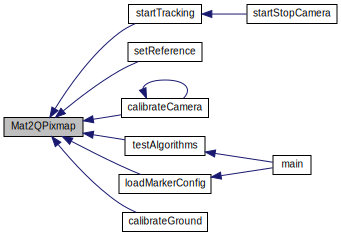
\includegraphics[width=350pt]{main_8cpp_a3e3cc959a7ab6f93ea52863d86373ce5_icgraph}
\end{center}
\end{figure}
\mbox{\Hypertarget{main_8cpp_a2104a5d9d6b9f1e29bc4cd858c59882e}\label{main_8cpp_a2104a5d9d6b9f1e29bc4cd858c59882e}} 
\index{main.\+cpp@{main.\+cpp}!project\+Coordinate\+Frame@{project\+Coordinate\+Frame}}
\index{project\+Coordinate\+Frame@{project\+Coordinate\+Frame}!main.\+cpp@{main.\+cpp}}
\subsubsection{\texorpdfstring{project\+Coordinate\+Frame()}{projectCoordinateFrame()}}
{\footnotesize\ttfamily void project\+Coordinate\+Frame (\begin{DoxyParamCaption}\item[{Mat}]{picture\+Frame }\end{DoxyParamCaption})}

Project the coordinate Co\+Sy origin and axis direction of the marker Co\+Sy with the rotation and translation of the object for visualization. 
\begin{DoxyParams}[1]{Parameters}
\mbox{\tt in}  & {\em picture\+Frame} & the image in which the Co\+Sy frame should be pasted. \\
\hline
\end{DoxyParams}


Definition at line 1076 of file main.\+cpp.


\begin{DoxyCode}
1077 \{
1078     projectPoints(\hyperlink{main_8cpp_ab34a04f5429de54d618fe1c9bd363c4e}{coordinateFrame}, \hyperlink{main_8cpp_ae095f10a005e68d20233dc15b4077ca6}{Rvec}, \hyperlink{main_8cpp_a9215ba881de0242c883e5b065d6d2ff9}{Tvec}, 
      \hyperlink{main_8cpp_a53e8957a459b639ca82d938157f3b085}{cameraMatrix}, \hyperlink{main_8cpp_a8d67876da148be9118bba1c0d017fb57}{distCoeffs}, \hyperlink{main_8cpp_a25a0b285905c7882d629b8f561425a2f}{coordinateFrameProjected});
1079     line(pictureFrame, \hyperlink{main_8cpp_a25a0b285905c7882d629b8f561425a2f}{coordinateFrameProjected}[0], 
      \hyperlink{main_8cpp_a25a0b285905c7882d629b8f561425a2f}{coordinateFrameProjected}[3], Scalar(0, 0, 255), 2); \textcolor{comment}{//!<z-axis}
1080 \textcolor{comment}{}    line(pictureFrame, \hyperlink{main_8cpp_a25a0b285905c7882d629b8f561425a2f}{coordinateFrameProjected}[0], 
      \hyperlink{main_8cpp_a25a0b285905c7882d629b8f561425a2f}{coordinateFrameProjected}[1], Scalar(255, 0, 0), 2); \textcolor{comment}{//!<x-axis}
1081 \textcolor{comment}{}    line(pictureFrame, \hyperlink{main_8cpp_a25a0b285905c7882d629b8f561425a2f}{coordinateFrameProjected}[0], 
      \hyperlink{main_8cpp_a25a0b285905c7882d629b8f561425a2f}{coordinateFrameProjected}[2], Scalar(0, 255, 0), 2); \textcolor{comment}{//!<y-axis}
1082 \textcolor{comment}{}\}
\end{DoxyCode}
Here is the caller graph for this function\+:\nopagebreak
\begin{figure}[H]
\begin{center}
\leavevmode
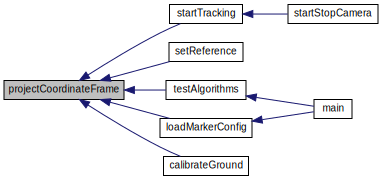
\includegraphics[width=350pt]{main_8cpp_a2104a5d9d6b9f1e29bc4cd858c59882e_icgraph}
\end{center}
\end{figure}
\mbox{\Hypertarget{main_8cpp_a54b6b6db348b48d21e1265e22829c61f}\label{main_8cpp_a54b6b6db348b48d21e1265e22829c61f}} 
\index{main.\+cpp@{main.\+cpp}!send\+Data\+U\+DP@{send\+Data\+U\+DP}}
\index{send\+Data\+U\+DP@{send\+Data\+U\+DP}!main.\+cpp@{main.\+cpp}}
\subsubsection{\texorpdfstring{send\+Data\+U\+D\+P()}{sendDataUDP()}}
{\footnotesize\ttfamily void send\+Data\+U\+DP (\begin{DoxyParamCaption}\item[{cv\+::\+Vec3d \&}]{Position,  }\item[{cv\+::\+Vec3d \&}]{Euler }\end{DoxyParamCaption})}

Send the position and attitude over U\+DP to every receiver, the safety receiver is handled on its own in the start\+Tracking function because its send rate is less than 100 Hz. 

Definition at line 1149 of file main.\+cpp.


\begin{DoxyCode}
1150 \{
1151     \hyperlink{main_8cpp_af38b495bf1b0e0651895215823059d30}{datagram}.clear();
1152     QDataStream out(&\hyperlink{main_8cpp_af38b495bf1b0e0651895215823059d30}{datagram}, QIODevice::WriteOnly);
1153     out.setVersion(QDataStream::Qt\_4\_3);
1154     out << (float)Position[0] << (\textcolor{keywordtype}{float})Position[1] << (float)Position[2];
1155     out << (float)Euler[0] << (\textcolor{keywordtype}{float})Euler[1] << (float)Euler[2]; \textcolor{comment}{//! Roll Pitch Heading}
1156 \textcolor{comment}{}    \hyperlink{main_8cpp_ae628b9aba095776b7134cf188486e174}{udpSocketObject}->writeDatagram(\hyperlink{main_8cpp_af38b495bf1b0e0651895215823059d30}{datagram}, 
      \hyperlink{main_8cpp_ab97ac0d82b1753d0eef37089be17e5e1}{IPAdressObject}, \hyperlink{main_8cpp_a9a00043c93a3362969c1c1fcd3a70fea}{portObject});
1157 \textcolor{comment}{}
1158 \textcolor{comment}{    //! if second receiver is activated send it also the tracking data}
1159 \textcolor{comment}{}    \textcolor{keywordflow}{if} (\hyperlink{main_8cpp_a436fb814ccc3f02617dade4dc6511143}{safety2Enable})
1160     \{
1161         \hyperlink{main_8cpp_a4260e46da4e0e430642b2d8d8d3c7dd1}{udpSocketSafety2}->writeDatagram(\hyperlink{main_8cpp_af38b495bf1b0e0651895215823059d30}{datagram}, 
      \hyperlink{main_8cpp_a354806cf8cbface3575f2541d8fbcbda}{IPAdressSafety2}, \hyperlink{main_8cpp_a2601be9c226be24c71ec8282f632e723}{portSafety2});
1162     \}
1163 
1164 \}
\end{DoxyCode}
Here is the caller graph for this function\+:\nopagebreak
\begin{figure}[H]
\begin{center}
\leavevmode
\includegraphics[width=350pt]{main_8cpp_a54b6b6db348b48d21e1265e22829c61f_icgraph}
\end{center}
\end{figure}
\mbox{\Hypertarget{main_8cpp_ad19da4e648bbdc80d3123eb94711588e}\label{main_8cpp_ad19da4e648bbdc80d3123eb94711588e}} 
\index{main.\+cpp@{main.\+cpp}!set\+Heading\+Offset@{set\+Heading\+Offset}}
\index{set\+Heading\+Offset@{set\+Heading\+Offset}!main.\+cpp@{main.\+cpp}}
\subsubsection{\texorpdfstring{set\+Heading\+Offset()}{setHeadingOffset()}}
{\footnotesize\ttfamily void set\+Heading\+Offset (\begin{DoxyParamCaption}\item[{double}]{d }\end{DoxyParamCaption})}

Add a heading offset to the attitude for the case it is wanted by the user. 
\begin{DoxyParams}[1]{Parameters}
\mbox{\tt in}  & {\em d} & denotes heading offset in degrees. \\
\hline
\end{DoxyParams}


Definition at line 1117 of file main.\+cpp.


\begin{DoxyCode}
1118 \{
1119     \hyperlink{main_8cpp_a377d62efbf6892902616cb71a4a5d5d7}{headingOffset} = d;
1120     d = d * 3.141592653589 / 180.0; \textcolor{comment}{//! Convert heading offset from degrees to rad}
1121 \textcolor{comment}{}\textcolor{comment}{}
1122 \textcolor{comment}{    //! Calculate rotation about x axis}
1123 \textcolor{comment}{}    Mat R\_x = (Mat\_<double>(3, 3) <<
1124         1, 0, 0,
1125         0, 1, 0,
1126         0, 0, 1
1127         );
1128 \textcolor{comment}{}
1129 \textcolor{comment}{    //! Calculate rotation about y axis}
1130 \textcolor{comment}{}    Mat R\_y = (Mat\_<double>(3, 3) <<
1131         1, 0, 0,
1132         0, 1, 0,
1133         0, 0, 1
1134         );
1135 \textcolor{comment}{}
1136 \textcolor{comment}{    //! Calculate rotation about z axis}
1137 \textcolor{comment}{}    Mat R\_z = (Mat\_<double>(3, 3) <<
1138         cos(d), -sin(d), 0,
1139         sin(d), cos(d), 0,
1140         0, 0, 1);
1141 
1142 \textcolor{comment}{}
1143 \textcolor{comment}{    //! Combined rotation matrix}
1144 \textcolor{comment}{}    \hyperlink{main_8cpp_a7b0c222d472eacfd5b0d73ed769baae0}{M\_HeadingOffset} = R\_z * R\_y * R\_x;
1145 \}
\end{DoxyCode}
Here is the caller graph for this function\+:\nopagebreak
\begin{figure}[H]
\begin{center}
\leavevmode
\includegraphics[width=350pt]{main_8cpp_ad19da4e648bbdc80d3123eb94711588e_icgraph}
\end{center}
\end{figure}
\mbox{\Hypertarget{main_8cpp_a1e6662e0f16887fe97c7bebe05065972}\label{main_8cpp_a1e6662e0f16887fe97c7bebe05065972}} 
\index{main.\+cpp@{main.\+cpp}!set\+Reference@{set\+Reference}}
\index{set\+Reference@{set\+Reference}!main.\+cpp@{main.\+cpp}}
\subsubsection{\texorpdfstring{set\+Reference()}{setReference()}}
{\footnotesize\ttfamily int set\+Reference (\begin{DoxyParamCaption}{ }\end{DoxyParamCaption})}

Determine the initial position of the object that serves as reference point or as ground frame origin. Computes the pose 200 times and then averages it. The position and attitude are from now on used as navigation Co\+Sy. 

Definition at line 590 of file main.\+cpp.


\begin{DoxyCode}
591 \{\textcolor{comment}{}
592 \textcolor{comment}{    //! initialize the variables with starting values}
593 \textcolor{comment}{}    \hyperlink{main_8cpp_acf655f393e3996144226399a338e8d3b}{gotOrder} = \textcolor{keyword}{false};
594     \hyperlink{main_8cpp_a9d2e25dbfda0ebcdbb488652c8b15fad}{posRef} = 0;
595     \hyperlink{main_8cpp_acd6966c004a57c4080ba204152200e7f}{eulerRef} = 0;
596     \hyperlink{main_8cpp_a4ee4d2abbe47b92c21b81c5c4389086e}{RmatRef} = 0;
597     \hyperlink{main_8cpp_ae095f10a005e68d20233dc15b4077ca6}{Rvec} = \hyperlink{main_8cpp_ae101daeaec726e27690c862b7edea825}{RvecOriginal};
598     \hyperlink{main_8cpp_a9215ba881de0242c883e5b065d6d2ff9}{Tvec} = \hyperlink{main_8cpp_a043bf1deaf5d42d47e0cce8982c1f18b}{TvecOriginal};
599 
600     \hyperlink{main_8cpp_a0416912fce6274568e80019b10ba294f}{determineExposure}();
601 
602     \hyperlink{main_8cpp_a8fc3524f4e679a41dcc8d0f302d637ed}{ss}.str(\textcolor{stringliteral}{""});
603     \hyperlink{main_8cpp_af29e7fc07ae0979d5fb61b473241d33d}{commObj}.\hyperlink{classcomm_object_aec354c7099b3039083cc4224e071e022}{addLog}(\textcolor{stringliteral}{"Started reference coordinate determination."});
604 
605     CameraLibrary\_EnableDevelopment();\textcolor{comment}{}
606 \textcolor{comment}{    //! Initialize Camera SDK ==--}
607 \textcolor{comment}{}    CameraLibrary::CameraManager::X();
608 \textcolor{comment}{}
609 \textcolor{comment}{    //! At this point the Camera SDK is actively looking for all connected cameras and will initialize}
610 \textcolor{comment}{    //! them on it's own.}
611 \textcolor{comment}{}\textcolor{comment}{}
612 \textcolor{comment}{    //! Get a connected camera ================----}
613 \textcolor{comment}{}    CameraManager::X().WaitForInitialization();
614     Camera *camera = CameraManager::X().GetCamera();
615 \textcolor{comment}{}
616 \textcolor{comment}{    //! If no device connected, pop a message box and exit ==--}
617 \textcolor{comment}{}    \textcolor{keywordflow}{if} (camera == 0)
618     \{
619         \hyperlink{main_8cpp_af29e7fc07ae0979d5fb61b473241d33d}{commObj}.\hyperlink{classcomm_object_aec354c7099b3039083cc4224e071e022}{addLog}(\textcolor{stringliteral}{"No camera found!"});
620         \textcolor{keywordflow}{return} 1;
621     \}
622 \textcolor{comment}{}
623 \textcolor{comment}{    //! Determine camera resolution to size application window ==----}
624 \textcolor{comment}{}    \textcolor{keywordtype}{int} cameraWidth = camera->Width();
625     \textcolor{keywordtype}{int} cameraHeight = camera->Height();
626     camera->GetDistortionModel(\hyperlink{main_8cpp_a9fba099569a2da23e458c2571f69652a}{distModel});
627     cv::Mat matFrame(cv::Size(cameraWidth, cameraHeight), CV\_8UC1);
628 \textcolor{comment}{}
629 \textcolor{comment}{    //! Set camera mode to precision mode, it directly provides marker coordinates}
630 \textcolor{comment}{}    camera->SetVideoType(Core::PrecisionMode);
631 \textcolor{comment}{}
632 \textcolor{comment}{    //! Start camera output ==--}
633 \textcolor{comment}{}    camera->Start();
634 \textcolor{comment}{}
635 \textcolor{comment}{    //! Turn on some overlay text so it's clear things are     ===---}
636 \textcolor{comment}{    //! working even if there is nothing in the camera's view. ===---}
637 \textcolor{comment}{    //! Set some other parameters as well of the camera}
638 \textcolor{comment}{}    camera->SetTextOverlay(\textcolor{keyword}{true});
639     camera->SetFrameRate(\hyperlink{main_8cpp_aa5b833b78b107a1a04eb4edba151c0ba}{intFrameRate});
640     camera->SetIntensity(\hyperlink{main_8cpp_a4e18b0b26ecc511ca7d2f2205313e537}{intIntensity});
641     camera->SetIRFilter(\textcolor{keyword}{true});
642     camera->SetContinuousIR(\textcolor{keyword}{false});
643     camera->SetHighPowerMode(\textcolor{keyword}{false});
644 \textcolor{comment}{}
645 \textcolor{comment}{    //! sample some frames and calculate the position and attitude. then average those values and use that
       as zero position}
646 \textcolor{comment}{}    \textcolor{keywordtype}{int} numberSamples = 0;
647     \textcolor{keywordtype}{int} numberToSample = 200;
648     \textcolor{keywordtype}{double} projectionError = 0; \textcolor{comment}{//!< difference between the marker points as seen by the camera and the
       projected marker points with Rvec and Tvec}
649 \textcolor{comment}{}
650     \textcolor{keywordflow}{while} (numberSamples < numberToSample)
651     \{\textcolor{comment}{}
652 \textcolor{comment}{        //! Fetch a new frame from the camera ===---}
653 \textcolor{comment}{}        Frame *frame = camera->GetFrame();
654 
655         \textcolor{keywordflow}{if} (frame)
656         \{\textcolor{comment}{}
657 \textcolor{comment}{            //! Ok, we've received a new frame, lets do something}
658 \textcolor{comment}{            //! with it.}
659 \textcolor{comment}{}            \textcolor{keywordflow}{if} (frame->ObjectCount() == \hyperlink{main_8cpp_ae1d37a43f631aefe76b6e540da786064}{numberMarkers})
660             \{\textcolor{comment}{}
661 \textcolor{comment}{                //!for(int i=0; i<frame->ObjectCount(); i++)}
662 \textcolor{comment}{}                \textcolor{keywordflow}{for} (\textcolor{keywordtype}{int} i = 0; i < \hyperlink{main_8cpp_ae1d37a43f631aefe76b6e540da786064}{numberMarkers}; i++)
663                 \{
664                     cObject *obj = frame->Object(i);
665                     \hyperlink{main_8cpp_a54cb682bd037283c18b5a9a447ff5e5e}{list\_points2dUnsorted}[i] = cv::Point2d(obj->X(), obj->Y());
666                 \}
667 
668                 \textcolor{keywordflow}{if} (\hyperlink{main_8cpp_acf655f393e3996144226399a338e8d3b}{gotOrder} == \textcolor{keyword}{false})
669                 \{
670                     \hyperlink{main_8cpp_a11ff459289305229597defd39f510959}{determineOrder}();
671                 \}
672 \textcolor{comment}{}
673 \textcolor{comment}{                //! sort the 2d points with the correct indices as found in the preceeding order
       determination algorithm}
674 \textcolor{comment}{}                \textcolor{keywordflow}{for} (\textcolor{keywordtype}{int} w = 0; w < \hyperlink{main_8cpp_ae1d37a43f631aefe76b6e540da786064}{numberMarkers}; w++)
675                 \{
676                     \hyperlink{main_8cpp_ad583e75f176dafdb7de3f214673851de}{list\_points2d}[w] = \hyperlink{main_8cpp_a54cb682bd037283c18b5a9a447ff5e5e}{list\_points2dUnsorted}[
      \hyperlink{main_8cpp_ac06fee052099b9fc9f0826315bb64a4a}{pointOrderIndices}[w]];
677                 \}
678                 \hyperlink{main_8cpp_a85d3d8c8a0e3e9cfb6157c247470d934}{list\_points2dOld} = \hyperlink{main_8cpp_a54cb682bd037283c18b5a9a447ff5e5e}{list\_points2dUnsorted};
679 \textcolor{comment}{}
680 \textcolor{comment}{                //!Compute the pose from the 3D-2D corresponses}
681 \textcolor{comment}{}                solvePnP(\hyperlink{main_8cpp_a933edb4ba1c0589d59020164c2f1ff87}{list\_points3d}, \hyperlink{main_8cpp_ad583e75f176dafdb7de3f214673851de}{list\_points2d}, 
      \hyperlink{main_8cpp_a53e8957a459b639ca82d938157f3b085}{cameraMatrix}, \hyperlink{main_8cpp_a8d67876da148be9118bba1c0d017fb57}{distCoeffs}, \hyperlink{main_8cpp_ae095f10a005e68d20233dc15b4077ca6}{Rvec}, \hyperlink{main_8cpp_a9215ba881de0242c883e5b065d6d2ff9}{Tvec}, \hyperlink{main_8cpp_ab1cc9be1ff0871bc5de1eb4c2811ae3e}{useGuess}, 
      \hyperlink{main_8cpp_ab5e634b66221f494504aea1557af5df9}{methodPNP});
682 \textcolor{comment}{}
683 \textcolor{comment}{                //! project the marker 3d points with the solution into the camera image CoSy and calculate
       difference to true camera image}
684 \textcolor{comment}{}                projectPoints(\hyperlink{main_8cpp_a933edb4ba1c0589d59020164c2f1ff87}{list\_points3d}, \hyperlink{main_8cpp_ae095f10a005e68d20233dc15b4077ca6}{Rvec}, \hyperlink{main_8cpp_a9215ba881de0242c883e5b065d6d2ff9}{Tvec}, 
      \hyperlink{main_8cpp_a53e8957a459b639ca82d938157f3b085}{cameraMatrix}, \hyperlink{main_8cpp_a8d67876da148be9118bba1c0d017fb57}{distCoeffs}, \hyperlink{main_8cpp_a7b88d0425a68875639d40a17079df819}{list\_points2dProjected});
685                 projectionError = norm(\hyperlink{main_8cpp_a7b88d0425a68875639d40a17079df819}{list\_points2dProjected}, 
      \hyperlink{main_8cpp_ad583e75f176dafdb7de3f214673851de}{list\_points2d});
686 
687                 \textcolor{keywordtype}{double} maxValue = 0;
688                 \textcolor{keywordtype}{double} minValue = 0;
689                 minMaxLoc(\hyperlink{main_8cpp_a9215ba881de0242c883e5b065d6d2ff9}{Tvec}.at<\textcolor{keywordtype}{double}>(2), &minValue, &maxValue);
690 
691                 \textcolor{keywordflow}{if} (maxValue > 10000 || minValue < 0)
692                 \{
693                     \hyperlink{main_8cpp_a8fc3524f4e679a41dcc8d0f302d637ed}{ss}.str(\textcolor{stringliteral}{""});
694                     \hyperlink{main_8cpp_a8fc3524f4e679a41dcc8d0f302d637ed}{ss} << \textcolor{stringliteral}{"Negative z distance, thats not possible. Start the set zero routine again or
       restart Programm."};
695                     \hyperlink{main_8cpp_af29e7fc07ae0979d5fb61b473241d33d}{commObj}.\hyperlink{classcomm_object_aec354c7099b3039083cc4224e071e022}{addLog}(QString::fromStdString(\hyperlink{main_8cpp_a8fc3524f4e679a41dcc8d0f302d637ed}{ss}.str()));
696                     frame->Release();
697                     \textcolor{keywordflow}{return} 1;
698                 \}
699 
700                 \textcolor{keywordflow}{if} (projectionError > 3)
701                 \{
702                     \hyperlink{main_8cpp_af29e7fc07ae0979d5fb61b473241d33d}{commObj}.\hyperlink{classcomm_object_aec354c7099b3039083cc4224e071e022}{addLog}(\textcolor{stringliteral}{"Reprojection error is bigger than 3 pixel. Correct marker
       configuration loaded?\(\backslash\)nMarker position measured precisely?"});
703                     frame->Release();
704                     \textcolor{keywordflow}{return} 1;
705                 \}
706 
707                 \textcolor{keywordflow}{if} (norm(\hyperlink{main_8cpp_a1d543a183197268bcb54a06bf157852c}{positionOld}) - norm(\hyperlink{main_8cpp_a9215ba881de0242c883e5b065d6d2ff9}{Tvec}) < 0.05)   \textcolor{comment}{//!<Iterative Method needs time
       to converge to solution}
708 \textcolor{comment}{}                \{
709                     add(\hyperlink{main_8cpp_a9d2e25dbfda0ebcdbb488652c8b15fad}{posRef}, \hyperlink{main_8cpp_a9215ba881de0242c883e5b065d6d2ff9}{Tvec}, \hyperlink{main_8cpp_a9d2e25dbfda0ebcdbb488652c8b15fad}{posRef});
710                     add(\hyperlink{main_8cpp_acd6966c004a57c4080ba204152200e7f}{eulerRef}, \hyperlink{main_8cpp_ae095f10a005e68d20233dc15b4077ca6}{Rvec}, \hyperlink{main_8cpp_acd6966c004a57c4080ba204152200e7f}{eulerRef}); \textcolor{comment}{//!< That are not the values of yaw,
       roll and pitch yet! Rodriguez has to be called first. }
711 \textcolor{comment}{}                    numberSamples++;    \textcolor{comment}{//!<  one sample more :D}
712 \textcolor{comment}{}                    \hyperlink{main_8cpp_af29e7fc07ae0979d5fb61b473241d33d}{commObj}.\hyperlink{classcomm_object_acfc97f4310e2b7d841ecb8cf8be0088e}{progressUpdate}(numberSamples * 100 / numberToSample);
713                 \}
714                 \hyperlink{main_8cpp_a1d543a183197268bcb54a06bf157852c}{positionOld} = \hyperlink{main_8cpp_a9215ba881de0242c883e5b065d6d2ff9}{Tvec};
715 
716                 Mat cFrame(480, 640, CV\_8UC3, Scalar(0, 0, 0));
717                 \textcolor{keywordflow}{for} (\textcolor{keywordtype}{int} i = 0; i < \hyperlink{main_8cpp_ae1d37a43f631aefe76b6e540da786064}{numberMarkers}; i++)
718                 \{
719                     circle(cFrame, Point(\hyperlink{main_8cpp_ad583e75f176dafdb7de3f214673851de}{list\_points2d}[i].x, 
      \hyperlink{main_8cpp_ad583e75f176dafdb7de3f214673851de}{list\_points2d}[i].y), 6, Scalar(0, 225, 0), 3);
720                 \}
721                 \hyperlink{main_8cpp_a2104a5d9d6b9f1e29bc4cd858c59882e}{projectCoordinateFrame}(cFrame);
722                 projectPoints(\hyperlink{main_8cpp_a933edb4ba1c0589d59020164c2f1ff87}{list\_points3d}, \hyperlink{main_8cpp_ae095f10a005e68d20233dc15b4077ca6}{Rvec}, \hyperlink{main_8cpp_a9215ba881de0242c883e5b065d6d2ff9}{Tvec}, 
      \hyperlink{main_8cpp_a53e8957a459b639ca82d938157f3b085}{cameraMatrix}, \hyperlink{main_8cpp_a8d67876da148be9118bba1c0d017fb57}{distCoeffs}, \hyperlink{main_8cpp_ad583e75f176dafdb7de3f214673851de}{list\_points2d});
723                 \textcolor{keywordflow}{for} (\textcolor{keywordtype}{int} i = 0; i < \hyperlink{main_8cpp_ae1d37a43f631aefe76b6e540da786064}{numberMarkers}; i++)
724                 \{
725                     circle(cFrame, Point(\hyperlink{main_8cpp_ad583e75f176dafdb7de3f214673851de}{list\_points2d}[i].x, 
      \hyperlink{main_8cpp_ad583e75f176dafdb7de3f214673851de}{list\_points2d}[i].y), 3, Scalar(225, 0, 0), 3);
726                 \}
727                 \hyperlink{main_8cpp_af6430ad2592a955a3618549547dfc5be}{drawPositionText}(cFrame, \hyperlink{main_8cpp_ac6dab448fd1f9b3aed1205fbd8179f5d}{position}, 
      \hyperlink{main_8cpp_a0a53d01e06c71d6360afcb0fabf2aa8e}{eulerAngles}, projectionError);
728 
729                 QPixmap QPFrame;
730                 QPFrame = \hyperlink{main_8cpp_a3e3cc959a7ab6f93ea52863d86373ce5}{Mat2QPixmap}(cFrame);
731                 \hyperlink{main_8cpp_af29e7fc07ae0979d5fb61b473241d33d}{commObj}.\hyperlink{classcomm_object_a6f81522c2aa1668fa402f08710e6206b}{changeImage}(QPFrame);
732                 QCoreApplication::processEvents();
733 
734             \}
735             frame->Release();
736         \}
737     \}\textcolor{comment}{}
738 \textcolor{comment}{    //! Release camera ==--}
739 \textcolor{comment}{}    camera->Release();
740 \textcolor{comment}{}
741 \textcolor{comment}{    //!Divide by the number of samples to get the mean of the reference position}
742 \textcolor{comment}{}    divide(\hyperlink{main_8cpp_a9d2e25dbfda0ebcdbb488652c8b15fad}{posRef}, numberToSample, \hyperlink{main_8cpp_a9d2e25dbfda0ebcdbb488652c8b15fad}{posRef});
743     divide(\hyperlink{main_8cpp_acd6966c004a57c4080ba204152200e7f}{eulerRef}, numberToSample, \hyperlink{main_8cpp_acd6966c004a57c4080ba204152200e7f}{eulerRef}); \textcolor{comment}{//!< eulerRef is here in Axis Angle
       notation}
744 \textcolor{comment}{}
745     Rodrigues(\hyperlink{main_8cpp_acd6966c004a57c4080ba204152200e7f}{eulerRef}, \hyperlink{main_8cpp_a4ee4d2abbe47b92c21b81c5c4389086e}{RmatRef});                \textcolor{comment}{//!< axis angle to rotation matrix}
746 \textcolor{comment}{}\textcolor{comment}{    //!-- Euler Angles, finally }
747 \textcolor{comment}{}    \hyperlink{main_8cpp_ab2b71933055cf32cc8e5e2100fd7723f}{getEulerAngles}(\hyperlink{main_8cpp_a4ee4d2abbe47b92c21b81c5c4389086e}{RmatRef}, \hyperlink{main_8cpp_acd6966c004a57c4080ba204152200e7f}{eulerRef}); \textcolor{comment}{//!<  rotation matrix to euler}
748 \textcolor{comment}{}    \hyperlink{main_8cpp_a8fc3524f4e679a41dcc8d0f302d637ed}{ss}.str(\textcolor{stringliteral}{""});
749     \hyperlink{main_8cpp_a8fc3524f4e679a41dcc8d0f302d637ed}{ss} << \textcolor{stringliteral}{"RmatRef is:\(\backslash\)n"};
750     \hyperlink{main_8cpp_a8fc3524f4e679a41dcc8d0f302d637ed}{ss} << \hyperlink{main_8cpp_a4ee4d2abbe47b92c21b81c5c4389086e}{RmatRef} << \textcolor{stringliteral}{"\(\backslash\)n"};
751     \hyperlink{main_8cpp_a8fc3524f4e679a41dcc8d0f302d637ed}{ss} << \textcolor{stringliteral}{"Reference Position is:\(\backslash\)n"};
752     \hyperlink{main_8cpp_a8fc3524f4e679a41dcc8d0f302d637ed}{ss} << \hyperlink{main_8cpp_a9d2e25dbfda0ebcdbb488652c8b15fad}{posRef} << \textcolor{stringliteral}{"[mm] \(\backslash\)n"};
753     \hyperlink{main_8cpp_a8fc3524f4e679a41dcc8d0f302d637ed}{ss} << \textcolor{stringliteral}{"Reference Euler Angles are:\(\backslash\)n"};
754     \hyperlink{main_8cpp_a8fc3524f4e679a41dcc8d0f302d637ed}{ss} << \hyperlink{main_8cpp_acd6966c004a57c4080ba204152200e7f}{eulerRef} << \textcolor{stringliteral}{"[deg] \(\backslash\)n"};
755 \textcolor{comment}{}
756 \textcolor{comment}{    //! compute the difference between last obtained TVec and the average Value}
757 \textcolor{comment}{    //! When it is large the iterative method has not converged properly so it is advised to start the
       setReference() function once again}
758 \textcolor{comment}{}    \textcolor{keywordtype}{double} error = norm(posRef) - norm(\hyperlink{main_8cpp_a9215ba881de0242c883e5b065d6d2ff9}{Tvec});
759     \textcolor{keywordflow}{if} (error > 5.0)
760     \{
761         \hyperlink{main_8cpp_a8fc3524f4e679a41dcc8d0f302d637ed}{ss} << \textcolor{stringliteral}{"Caution, distance between reference position and last position is: "} << error << \textcolor{stringliteral}{"\(\backslash\)n Start
       the set zero routine once again."};
762     \}
763     \hyperlink{main_8cpp_af29e7fc07ae0979d5fb61b473241d33d}{commObj}.\hyperlink{classcomm_object_aec354c7099b3039083cc4224e071e022}{addLog}(QString::fromStdString(\hyperlink{main_8cpp_a8fc3524f4e679a41dcc8d0f302d637ed}{ss}.str()));
764     \hyperlink{main_8cpp_af29e7fc07ae0979d5fb61b473241d33d}{commObj}.\hyperlink{classcomm_object_acfc97f4310e2b7d841ecb8cf8be0088e}{progressUpdate}(0);
765     \textcolor{keywordflow}{return} 0;
766 \}
\end{DoxyCode}
Here is the call graph for this function\+:\nopagebreak
\begin{figure}[H]
\begin{center}
\leavevmode
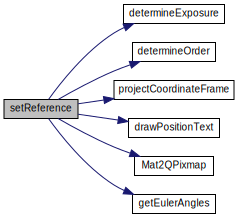
\includegraphics[width=350pt]{main_8cpp_a1e6662e0f16887fe97c7bebe05065972_cgraph}
\end{center}
\end{figure}
Here is the caller graph for this function\+:\nopagebreak
\begin{figure}[H]
\begin{center}
\leavevmode
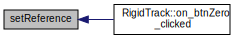
\includegraphics[width=306pt]{main_8cpp_a1e6662e0f16887fe97c7bebe05065972_icgraph}
\end{center}
\end{figure}
\mbox{\Hypertarget{main_8cpp_ae624b0189bc5e32cbbb1f178b9f1a360}\label{main_8cpp_ae624b0189bc5e32cbbb1f178b9f1a360}} 
\index{main.\+cpp@{main.\+cpp}!set\+Up\+U\+DP@{set\+Up\+U\+DP}}
\index{set\+Up\+U\+DP@{set\+Up\+U\+DP}!main.\+cpp@{main.\+cpp}}
\subsubsection{\texorpdfstring{set\+Up\+U\+D\+P()}{setUpUDP()}}
{\footnotesize\ttfamily void set\+Up\+U\+DP (\begin{DoxyParamCaption}{ }\end{DoxyParamCaption})}



Open the U\+DP ports for communication. 



Definition at line 1085 of file main.\+cpp.


\begin{DoxyCode}
1086 \{\textcolor{comment}{}
1087 \textcolor{comment}{    //! Initialise the QDataStream that stores the data to be send}
1088 \textcolor{comment}{}    QDataStream out(&\hyperlink{main_8cpp_af38b495bf1b0e0651895215823059d30}{datagram}, QIODevice::WriteOnly);
1089     out.setVersion(QDataStream::Qt\_4\_3);
1090 \textcolor{comment}{}
1091 \textcolor{comment}{    //! Create UDP slots}
1092 \textcolor{comment}{}    \hyperlink{main_8cpp_af29e7fc07ae0979d5fb61b473241d33d}{commObj}.\hyperlink{classcomm_object_aec354c7099b3039083cc4224e071e022}{addLog}(\textcolor{stringliteral}{"Opening UDP ports."});
1093     \hyperlink{main_8cpp_ae628b9aba095776b7134cf188486e174}{udpSocketObject} = \textcolor{keyword}{new} QUdpSocket(0);
1094     \hyperlink{main_8cpp_ae628b9aba095776b7134cf188486e174}{udpSocketObject}->connectToHost(\hyperlink{main_8cpp_ab97ac0d82b1753d0eef37089be17e5e1}{IPAdressObject}, 
      \hyperlink{main_8cpp_a9a00043c93a3362969c1c1fcd3a70fea}{portObject});
1095     \hyperlink{main_8cpp_af29e7fc07ae0979d5fb61b473241d33d}{commObj}.\hyperlink{classcomm_object_aec354c7099b3039083cc4224e071e022}{addLog}(\textcolor{stringliteral}{"Opened first receiver UDP port."});
1096 
1097     \hyperlink{main_8cpp_a6aa0c3a69dc10d5c4432dcf62e2155d3}{udpSocketSafety} = \textcolor{keyword}{new} QUdpSocket(0);
1098     \hyperlink{main_8cpp_a4260e46da4e0e430642b2d8d8d3c7dd1}{udpSocketSafety2} = \textcolor{keyword}{new} QUdpSocket(0);
1099 \textcolor{comment}{}
1100 \textcolor{comment}{    //! if the safety feature is activated open the udp port}
1101 \textcolor{comment}{}    \textcolor{keywordflow}{if} (\hyperlink{main_8cpp_aa6266eedab8b3c011be53baffbfc42ab}{safetyEnable})
1102     \{
1103         \hyperlink{main_8cpp_a6aa0c3a69dc10d5c4432dcf62e2155d3}{udpSocketSafety}->connectToHost(\hyperlink{main_8cpp_afefb1102a8a4a71b55d6f24f46404cc5}{IPAdressSafety}, 
      \hyperlink{main_8cpp_a137bc8cc9d53ad9b176c988a99bc7142}{portSafety});
1104         \hyperlink{main_8cpp_af29e7fc07ae0979d5fb61b473241d33d}{commObj}.\hyperlink{classcomm_object_aec354c7099b3039083cc4224e071e022}{addLog}(\textcolor{stringliteral}{"Opened safety UDP port."});
1105     \}
1106 \textcolor{comment}{}
1107 \textcolor{comment}{    //! if the second receiver feature is activated open the udp port}
1108 \textcolor{comment}{}    \textcolor{keywordflow}{if} (\hyperlink{main_8cpp_a436fb814ccc3f02617dade4dc6511143}{safety2Enable})
1109     \{
1110         \hyperlink{main_8cpp_a4260e46da4e0e430642b2d8d8d3c7dd1}{udpSocketSafety2}->connectToHost(\hyperlink{main_8cpp_a354806cf8cbface3575f2541d8fbcbda}{IPAdressSafety2}, 
      \hyperlink{main_8cpp_a2601be9c226be24c71ec8282f632e723}{portSafety2});
1111         \hyperlink{main_8cpp_af29e7fc07ae0979d5fb61b473241d33d}{commObj}.\hyperlink{classcomm_object_aec354c7099b3039083cc4224e071e022}{addLog}(\textcolor{stringliteral}{"Opened second receiver UDP port."});
1112     \}
1113 \}
\end{DoxyCode}
Here is the call graph for this function\+:\nopagebreak
\begin{figure}[H]
\begin{center}
\leavevmode
\includegraphics[width=288pt]{main_8cpp_ae624b0189bc5e32cbbb1f178b9f1a360_cgraph}
\end{center}
\end{figure}
Here is the caller graph for this function\+:\nopagebreak
\begin{figure}[H]
\begin{center}
\leavevmode
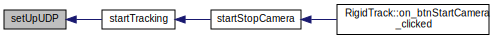
\includegraphics[width=350pt]{main_8cpp_ae624b0189bc5e32cbbb1f178b9f1a360_icgraph}
\end{center}
\end{figure}
\mbox{\Hypertarget{main_8cpp_a25183e8d0b386ef12b557efc712a0261}\label{main_8cpp_a25183e8d0b386ef12b557efc712a0261}} 
\index{main.\+cpp@{main.\+cpp}!start\+Stop\+Camera@{start\+Stop\+Camera}}
\index{start\+Stop\+Camera@{start\+Stop\+Camera}!main.\+cpp@{main.\+cpp}}
\subsubsection{\texorpdfstring{start\+Stop\+Camera()}{startStopCamera()}}
{\footnotesize\ttfamily void start\+Stop\+Camera (\begin{DoxyParamCaption}{ }\end{DoxyParamCaption})}



Start or stop the tracking depending on if the camera is currently running or not. 



Definition at line 574 of file main.\+cpp.


\begin{DoxyCode}
575 \{\textcolor{comment}{}
576 \textcolor{comment}{    //! tracking is not running so start it}
577 \textcolor{comment}{}    \textcolor{keywordflow}{if} (\hyperlink{main_8cpp_a6b1342fd3f76c3ce13245825cff8e400}{exitRequested})
578     \{
579         \hyperlink{main_8cpp_a6b1342fd3f76c3ce13245825cff8e400}{exitRequested} = \textcolor{keyword}{false};
580         \hyperlink{main_8cpp_a3d3afd29ce54eb7fc5cc7e74ab666586}{startTracking}();
581     \}
582     \textcolor{keywordflow}{else}  \textcolor{comment}{//!< tracking is currently running, set exitRequest to true so the while loop in startTracking()
       exits}
583 \textcolor{comment}{}    \{
584         \hyperlink{main_8cpp_a6b1342fd3f76c3ce13245825cff8e400}{exitRequested} = \textcolor{keyword}{true};
585     \}
586 \}
\end{DoxyCode}
Here is the call graph for this function\+:\nopagebreak
\begin{figure}[H]
\begin{center}
\leavevmode
\includegraphics[width=350pt]{main_8cpp_a25183e8d0b386ef12b557efc712a0261_cgraph}
\end{center}
\end{figure}
Here is the caller graph for this function\+:\nopagebreak
\begin{figure}[H]
\begin{center}
\leavevmode
\includegraphics[width=350pt]{main_8cpp_a25183e8d0b386ef12b557efc712a0261_icgraph}
\end{center}
\end{figure}
\mbox{\Hypertarget{main_8cpp_a3d3afd29ce54eb7fc5cc7e74ab666586}\label{main_8cpp_a3d3afd29ce54eb7fc5cc7e74ab666586}} 
\index{main.\+cpp@{main.\+cpp}!start\+Tracking@{start\+Tracking}}
\index{start\+Tracking@{start\+Tracking}!main.\+cpp@{main.\+cpp}}
\subsubsection{\texorpdfstring{start\+Tracking()}{startTracking()}}
{\footnotesize\ttfamily int start\+Tracking (\begin{DoxyParamCaption}{ }\end{DoxyParamCaption})}

Start the loop that fetches frames, computes the position etc and sends it to other computers. This function is the core of this program, hence the pose estimation is done here. 

Definition at line 256 of file main.\+cpp.


\begin{DoxyCode}
256                     \{
257 
258 
259     \hyperlink{main_8cpp_acf655f393e3996144226399a338e8d3b}{gotOrder} = \textcolor{keyword}{false}; \textcolor{comment}{//! The order of points, hence which entry in list\_points3d corresponds to
       which in list\_points2d is not calculated yet}
260 \textcolor{comment}{}    \hyperlink{main_8cpp_ae095f10a005e68d20233dc15b4077ca6}{Rvec} = \hyperlink{main_8cpp_ae101daeaec726e27690c862b7edea825}{RvecOriginal}; \textcolor{comment}{//! Use the value of Rvec that was set in main() as starting value
       for the solvePnP algorithm}
261 \textcolor{comment}{}    \hyperlink{main_8cpp_a9215ba881de0242c883e5b065d6d2ff9}{Tvec} = \hyperlink{main_8cpp_a043bf1deaf5d42d47e0cce8982c1f18b}{TvecOriginal}; \textcolor{comment}{//! Use the value of Tvec that was set in main() as starting value
       for the solvePnP algorithm}
262 \textcolor{comment}{}    GetLocalTime(&\hyperlink{main_8cpp_aba7ea4b1074abf42199ab9ab295e9c33}{logDate});  \textcolor{comment}{//! Get the current date and time to name the log file}
263 \textcolor{comment}{}\textcolor{comment}{}
264 \textcolor{comment}{    //! Concat the log file name as followed. The file is saved in the folder /logs in the Rigid Track
       installation folder}
265 \textcolor{comment}{}    \hyperlink{main_8cpp_a10895c5c32e9441213c79f05d2b5ba45}{logFileName} = \textcolor{stringliteral}{"./logs/positionLog\_"} + QString::number(\hyperlink{main_8cpp_aba7ea4b1074abf42199ab9ab295e9c33}{logDate}.wDay) + \textcolor{stringliteral}{"\_"} + 
      QString::number(\hyperlink{main_8cpp_aba7ea4b1074abf42199ab9ab295e9c33}{logDate}.wMonth) + \textcolor{stringliteral}{"\_"} + QString::number(\hyperlink{main_8cpp_aba7ea4b1074abf42199ab9ab295e9c33}{logDate}.wYear);
266     \hyperlink{main_8cpp_a10895c5c32e9441213c79f05d2b5ba45}{logFileName} += \textcolor{stringliteral}{"\_"} + QString::number(\hyperlink{main_8cpp_aba7ea4b1074abf42199ab9ab295e9c33}{logDate}.wHour) + \textcolor{stringliteral}{"\_"} + QString::number(
      \hyperlink{main_8cpp_aba7ea4b1074abf42199ab9ab295e9c33}{logDate}.wMinute) + \textcolor{stringliteral}{"\_"} + QString::number(\hyperlink{main_8cpp_aba7ea4b1074abf42199ab9ab295e9c33}{logDate}.wSecond) + \textcolor{stringliteral}{".txt"};
267     \hyperlink{main_8cpp_a7a642b2c947e62ff5ec692ec95783bd0}{logName} = \hyperlink{main_8cpp_a10895c5c32e9441213c79f05d2b5ba45}{logFileName}.toStdString(); \textcolor{comment}{//! Convert the QString to a standard string}
268 \textcolor{comment}{}
269     \hyperlink{main_8cpp_a0416912fce6274568e80019b10ba294f}{determineExposure}(); \textcolor{comment}{//! Get the exposure where the right amount of markers is
       detected}
270 \textcolor{comment}{}\textcolor{comment}{}
271 \textcolor{comment}{    //! For OptiTrack Ethernet cameras, it's important to enable development mode if you}
272 \textcolor{comment}{    //! want to stop execution for an extended time while debugging without disconnecting}
273 \textcolor{comment}{    //! the Ethernet devices.  Lets do that now:}
274 \textcolor{comment}{}
275     CameraLibrary\_EnableDevelopment();
276     CameraLibrary::CameraManager::X(); \textcolor{comment}{//! Initialize Camera SDK}
277 \textcolor{comment}{}\textcolor{comment}{}
278 \textcolor{comment}{    //! At this point the Camera SDK is actively looking for all connected cameras and will initialize}
279 \textcolor{comment}{    //! them on it's own}
280 \textcolor{comment}{}\textcolor{comment}{}
281 \textcolor{comment}{    //! Get a connected camera}
282 \textcolor{comment}{}    CameraManager::X().WaitForInitialization();
283     Camera *camera = CameraManager::X().GetCamera();
284 \textcolor{comment}{}
285 \textcolor{comment}{    //! If no camera can be found, inform user in message log and exit function}
286 \textcolor{comment}{}    \textcolor{keywordflow}{if} (camera == 0)
287     \{
288         \hyperlink{main_8cpp_af29e7fc07ae0979d5fb61b473241d33d}{commObj}.\hyperlink{classcomm_object_aec354c7099b3039083cc4224e071e022}{addLog}(\textcolor{stringliteral}{"No camera found!"});
289         \textcolor{keywordflow}{return} 1;
290     \}
291 \textcolor{comment}{}
292 \textcolor{comment}{    //! Determine camera resolution to size application window }
293 \textcolor{comment}{}    \textcolor{keywordtype}{int} cameraWidth = camera->Width();
294     \textcolor{keywordtype}{int} cameraHeight = camera->Height();
295 
296     camera->SetVideoType(Core::PrecisionMode);  \textcolor{comment}{//! Set the camera mode to precision mode, it used
       greyscale imformation for marker property calculations}
297 \textcolor{comment}{}
298     camera->Start(); \textcolor{comment}{//! Start camera output}
299 \textcolor{comment}{}\textcolor{comment}{}
300 \textcolor{comment}{    //! Turn on some overlay text so it's clear things are}
301 \textcolor{comment}{    //! working even if there is nothing in the camera's view}
302 \textcolor{comment}{}    camera->SetTextOverlay(\textcolor{keyword}{true});
303     camera->SetExposure(\hyperlink{main_8cpp_afcaebd6cfd12b2e558363a06db8396ea}{intExposure});    \textcolor{comment}{//! Set the camera exposure}
304 \textcolor{comment}{}    camera->SetIntensity(\hyperlink{main_8cpp_a4e18b0b26ecc511ca7d2f2205313e537}{intIntensity}); \textcolor{comment}{//! Set the camera infrared LED intensity}
305 \textcolor{comment}{}    camera->SetFrameRate(\hyperlink{main_8cpp_aa5b833b78b107a1a04eb4edba151c0ba}{intFrameRate}); \textcolor{comment}{//! Set the camera framerate to 100 Hz}
306 \textcolor{comment}{}    camera->SetIRFilter(\textcolor{keyword}{true});  \textcolor{comment}{//! Enable the filter that blocks visible light and only passes infrared
       light}
307 \textcolor{comment}{}    camera->SetHighPowerMode(\textcolor{keyword}{true}); \textcolor{comment}{//! Enable high power mode of the LEDs}
308 \textcolor{comment}{}    camera->SetContinuousIR(\textcolor{keyword}{false}); \textcolor{comment}{//! Disable continuous LED light}
309 \textcolor{comment}{}    camera->SetThreshold(\hyperlink{main_8cpp_ac61559ce6020b8ec00161bc3a994ddcc}{intThreshold}); \textcolor{comment}{//! Set threshold for marker detection}
310 \textcolor{comment}{}\textcolor{comment}{}
311 \textcolor{comment}{    //! Create a new matrix that stores the grayscale picture from the camera}
312 \textcolor{comment}{}    Mat matFrame = Mat::zeros(cv::Size(cameraWidth, cameraHeight), CV\_8UC1);
313     QPixmap QPFrame; \textcolor{comment}{//! QPixmap is the corresponding Qt class that saves images}
314 \textcolor{comment}{}\textcolor{comment}{    //! Matrix that stores the colored picture, hence marker points, coordinate frame and reprojected
       points}
315 \textcolor{comment}{}    Mat cFrame(480, 640, CV\_8UC3, Scalar(0, 0, 0));
316 
317     \textcolor{keywordtype}{int} v = 0;  \textcolor{comment}{//! Helper variable used to kick safety switch}
318 \textcolor{comment}{}\textcolor{comment}{    //! Variables for the min and max values that are needed for sanity checks}
319 \textcolor{comment}{}    \textcolor{keywordtype}{double} maxValue = 0;
320     \textcolor{keywordtype}{double} minValue = 0;
321     \textcolor{keywordtype}{int} framesDropped = 0; \textcolor{comment}{//! Ff a marker is not visible or accuracy is bad increase this counter}
322 \textcolor{comment}{}    \textcolor{keywordtype}{double} projectionError = 0; \textcolor{comment}{//! Equals the quality of the tracking}
323 \textcolor{comment}{}
324     \hyperlink{main_8cpp_ae624b0189bc5e32cbbb1f178b9f1a360}{setUpUDP}(); \textcolor{comment}{//! Open sockets and ports for UDP communication}
325 \textcolor{comment}{}
326     \textcolor{keywordflow}{if} (\hyperlink{main_8cpp_aa6266eedab8b3c011be53baffbfc42ab}{safetyEnable}) \textcolor{comment}{//! If the safety feature is enabled send the starting message}
327 \textcolor{comment}{}    \{\textcolor{comment}{}
328 \textcolor{comment}{        //! Send enable message, hence send a 9 and then a 1 }
329 \textcolor{comment}{}        \hyperlink{main_8cpp_ad44c6ce322034044d573e6d4678d630b}{data}.setNum((\textcolor{keywordtype}{int})(9));
330         \hyperlink{main_8cpp_a6aa0c3a69dc10d5c4432dcf62e2155d3}{udpSocketSafety}->write(\hyperlink{main_8cpp_ad44c6ce322034044d573e6d4678d630b}{data});
331         \hyperlink{main_8cpp_ad44c6ce322034044d573e6d4678d630b}{data}.setNum((\textcolor{keywordtype}{int})(1));
332         \hyperlink{main_8cpp_a6aa0c3a69dc10d5c4432dcf62e2155d3}{udpSocketSafety}->write(\hyperlink{main_8cpp_ad44c6ce322034044d573e6d4678d630b}{data});
333     \}
334 \textcolor{comment}{}
335 \textcolor{comment}{    //! Fetch a new frame from the camera}
336 \textcolor{comment}{}    \textcolor{keywordtype}{bool} gotTime = \textcolor{keyword}{false}; \textcolor{comment}{//! Get the timestamp of the first frame. This time is subtracted from every
       subseeding frame so the time starts at 0 in the logs}
337 \textcolor{comment}{}    \textcolor{keywordflow}{while} (!gotTime) \textcolor{comment}{//! While no new frame is received loop }
338 \textcolor{comment}{}    \{
339         Frame *frame = camera->GetFrame(); \textcolor{comment}{//! Get a new camera frame}
340 \textcolor{comment}{}        \textcolor{keywordflow}{if} (frame)  \textcolor{comment}{//! There is actually a new frame}
341 \textcolor{comment}{}        \{
342             \hyperlink{main_8cpp_ac7de3790df75e7d70bfe280b9af47a56}{timeFirstFrame} = frame->TimeStamp(); \textcolor{comment}{//! Get the time stamp for the first frame.
       It is subtracted for the following frames}
343 \textcolor{comment}{}            frame->Release();   \textcolor{comment}{//! Release the frame so the camera can continue}
344 \textcolor{comment}{}            gotTime = \textcolor{keyword}{true}; \textcolor{comment}{//! Exit the while loop}
345 \textcolor{comment}{}        \}
346     \}
347 \textcolor{comment}{}
348 \textcolor{comment}{    //! Now enter the main loop that processes each frame and computes the pose, sends it and logs stuff}
349 \textcolor{comment}{}    \textcolor{keywordflow}{while} (!\hyperlink{main_8cpp_a6b1342fd3f76c3ce13245825cff8e400}{exitRequested}) \textcolor{comment}{//! Check if the user has not pressed "Stop Tracking" yet}
350 \textcolor{comment}{}    \{
351 
352         Frame *frame = camera->GetFrame(); \textcolor{comment}{//! Fetch a new frame from the camera}
353 \textcolor{comment}{}
354         \textcolor{keywordflow}{if} (frame) \textcolor{comment}{//! Did we got a new frame or does the camera still need more time}
355 \textcolor{comment}{}        \{
356             framesDropped++; \textcolor{comment}{//! Increase by one, if everything is okay it is decreased at the end of the
       loop again}
357 \textcolor{comment}{}\textcolor{comment}{}
358 \textcolor{comment}{            //! Only use this frame it the right number of markers is found in the picture}
359 \textcolor{comment}{}            \textcolor{keywordflow}{if} (frame->ObjectCount() == \hyperlink{main_8cpp_ae1d37a43f631aefe76b6e540da786064}{numberMarkers})
360             \{\textcolor{comment}{}
361 \textcolor{comment}{                //! Get the marker points in 2D in the camera image frame and store them in the
       list\_points2dUnsorted vector}
362 \textcolor{comment}{                //! The order of points that come from the camera corresponds to the Y coordinate}
363 \textcolor{comment}{}                \textcolor{keywordflow}{for} (\textcolor{keywordtype}{int} i = 0; i < \hyperlink{main_8cpp_ae1d37a43f631aefe76b6e540da786064}{numberMarkers}; i++)
364                 \{
365                     cObject *obj = frame->Object(i);
366                     \hyperlink{main_8cpp_a54cb682bd037283c18b5a9a447ff5e5e}{list\_points2dUnsorted}[i] = cv::Point2d(obj->X(), obj->Y());
367                 \}
368 
369                 \textcolor{keywordflow}{if} (\hyperlink{main_8cpp_acf655f393e3996144226399a338e8d3b}{gotOrder} == \textcolor{keyword}{false}) \textcolor{comment}{//! Was the order already determined? This is false for the
       first frame and from then on true}
370 \textcolor{comment}{}                \{
371                     \hyperlink{main_8cpp_a11ff459289305229597defd39f510959}{determineOrder}(); \textcolor{comment}{//! Now compute the order}
372 \textcolor{comment}{}                \}
373 \textcolor{comment}{}
374 \textcolor{comment}{                //! Sort the 2d points with the correct indices as found in the preceeding order
       determination algorithm}
375 \textcolor{comment}{}                \textcolor{keywordflow}{for} (\textcolor{keywordtype}{int} w = 0; w < \hyperlink{main_8cpp_ae1d37a43f631aefe76b6e540da786064}{numberMarkers}; w++)
376                 \{
377                     \hyperlink{main_8cpp_ad583e75f176dafdb7de3f214673851de}{list\_points2d}[w] = \hyperlink{main_8cpp_a54cb682bd037283c18b5a9a447ff5e5e}{list\_points2dUnsorted}[
      \hyperlink{main_8cpp_ac06fee052099b9fc9f0826315bb64a4a}{pointOrderIndices}[w]]; \textcolor{comment}{//! pointOrderIndices was calculated in determineOrder()}
378 \textcolor{comment}{}                \}
379                 \hyperlink{main_8cpp_a85d3d8c8a0e3e9cfb6157c247470d934}{list\_points2dOld} = \hyperlink{main_8cpp_a54cb682bd037283c18b5a9a447ff5e5e}{list\_points2dUnsorted};
380 \textcolor{comment}{}
381 \textcolor{comment}{                //! The first time the 2D-3D corresspondence was determined with gotOrder was okay. }
382 \textcolor{comment}{                //! But this order can change as the object moves and the marker objects appear in a}
383 \textcolor{comment}{                //! different order in the frame->Object() array.}
384 \textcolor{comment}{                //! The solution is that: When a marker point (in the camera image, hence in 2D) was at}
385 \textcolor{comment}{                //! a position then it wont move that much from one frame to the other.}
386 \textcolor{comment}{                //! So for the new frame we take a marker object and check which marker was closest this
       point  }
387 \textcolor{comment}{                //! in the old image frame? This is probably the same (true) marker. And we do that for
       every other marker as well.}
388 \textcolor{comment}{                //! When tracking is good and no frames are dropped because of missing markers this should
       work every frame.}
389 \textcolor{comment}{}                \textcolor{keywordflow}{for} (\textcolor{keywordtype}{int} j = 0; j < \hyperlink{main_8cpp_ae1d37a43f631aefe76b6e540da786064}{numberMarkers}; j++)
390                 \{
391                     \hyperlink{main_8cpp_ab826a7ca5876afdd6c0bccf04b73b30b}{minPointDistance} = 5000; \textcolor{comment}{//! The sum of point distances is set to
       something unrealistic large}
392 \textcolor{comment}{}                    \textcolor{keywordflow}{for} (\textcolor{keywordtype}{int} k = 0; k < \hyperlink{main_8cpp_ae1d37a43f631aefe76b6e540da786064}{numberMarkers}; k++)
393                     \{\textcolor{comment}{}
394 \textcolor{comment}{                        //! Calculate N\_2 norm of unsorted points minus old points}
395 \textcolor{comment}{}                        \hyperlink{main_8cpp_afe37bd67ad83a2d897cf5977cba70ef3}{currentPointDistance} = norm(
      \hyperlink{main_8cpp_a54cb682bd037283c18b5a9a447ff5e5e}{list\_points2dUnsorted}[\hyperlink{main_8cpp_ac06fee052099b9fc9f0826315bb64a4a}{pointOrderIndices}[j]] - 
      \hyperlink{main_8cpp_a85d3d8c8a0e3e9cfb6157c247470d934}{list\_points2dOld}[k]);\textcolor{comment}{}
396 \textcolor{comment}{                        //! If the norm is smaller than minPointDistance the correspondence is more likely
       to be correct}
397 \textcolor{comment}{}                        \textcolor{keywordflow}{if} (\hyperlink{main_8cpp_afe37bd67ad83a2d897cf5977cba70ef3}{currentPointDistance} < 
      \hyperlink{main_8cpp_ab826a7ca5876afdd6c0bccf04b73b30b}{minPointDistance})
398                         \{\textcolor{comment}{}
399 \textcolor{comment}{                            //! Update the array that saves the new point order}
400 \textcolor{comment}{}                            \hyperlink{main_8cpp_ab826a7ca5876afdd6c0bccf04b73b30b}{minPointDistance} = 
      \hyperlink{main_8cpp_afe37bd67ad83a2d897cf5977cba70ef3}{currentPointDistance};
401                             \hyperlink{main_8cpp_acc9e758efd664582db86f976cec195fa}{pointOrderIndicesNew}[j] = k;
402                         \}
403                     \}
404                 \}
405 \textcolor{comment}{}
406 \textcolor{comment}{                //! Now the new order is found, set the point order to the new value}
407 \textcolor{comment}{}                \textcolor{keywordflow}{for} (\textcolor{keywordtype}{int} k = 0; k < \hyperlink{main_8cpp_ae1d37a43f631aefe76b6e540da786064}{numberMarkers}; k++)
408                 \{
409                     \hyperlink{main_8cpp_ac06fee052099b9fc9f0826315bb64a4a}{pointOrderIndices}[k] = \hyperlink{main_8cpp_acc9e758efd664582db86f976cec195fa}{pointOrderIndicesNew}[k];
410                     \hyperlink{main_8cpp_ad583e75f176dafdb7de3f214673851de}{list\_points2d}[k] = \hyperlink{main_8cpp_a54cb682bd037283c18b5a9a447ff5e5e}{list\_points2dUnsorted}[
      \hyperlink{main_8cpp_ac06fee052099b9fc9f0826315bb64a4a}{pointOrderIndices}[k]];
411                 \}
412 \textcolor{comment}{}
413 \textcolor{comment}{                //! Save the unsorted position of the marker points for the next loop}
414 \textcolor{comment}{}                \hyperlink{main_8cpp_a85d3d8c8a0e3e9cfb6157c247470d934}{list\_points2dOld} = \hyperlink{main_8cpp_a54cb682bd037283c18b5a9a447ff5e5e}{list\_points2dUnsorted};
415 \textcolor{comment}{}
416 \textcolor{comment}{                //!Compute the object pose from the 3D-2D corresponses}
417 \textcolor{comment}{}                solvePnP(\hyperlink{main_8cpp_a933edb4ba1c0589d59020164c2f1ff87}{list\_points3d}, \hyperlink{main_8cpp_ad583e75f176dafdb7de3f214673851de}{list\_points2d}, 
      \hyperlink{main_8cpp_a53e8957a459b639ca82d938157f3b085}{cameraMatrix}, \hyperlink{main_8cpp_a8d67876da148be9118bba1c0d017fb57}{distCoeffs}, \hyperlink{main_8cpp_ae095f10a005e68d20233dc15b4077ca6}{Rvec}, \hyperlink{main_8cpp_a9215ba881de0242c883e5b065d6d2ff9}{Tvec}, \hyperlink{main_8cpp_ab1cc9be1ff0871bc5de1eb4c2811ae3e}{useGuess}, 
      \hyperlink{main_8cpp_ab5e634b66221f494504aea1557af5df9}{methodPNP});
418 \textcolor{comment}{}
419 \textcolor{comment}{                //! Project the marker 3d points with the solution into the camera image CoSy and calculate
       difference to true camera image}
420 \textcolor{comment}{}                projectPoints(\hyperlink{main_8cpp_a933edb4ba1c0589d59020164c2f1ff87}{list\_points3d}, \hyperlink{main_8cpp_ae095f10a005e68d20233dc15b4077ca6}{Rvec}, \hyperlink{main_8cpp_a9215ba881de0242c883e5b065d6d2ff9}{Tvec}, 
      \hyperlink{main_8cpp_a53e8957a459b639ca82d938157f3b085}{cameraMatrix}, \hyperlink{main_8cpp_a8d67876da148be9118bba1c0d017fb57}{distCoeffs}, \hyperlink{main_8cpp_a7b88d0425a68875639d40a17079df819}{list\_points2dProjected});
421                 projectionError = norm(\hyperlink{main_8cpp_a7b88d0425a68875639d40a17079df819}{list\_points2dProjected}, 
      \hyperlink{main_8cpp_ad583e75f176dafdb7de3f214673851de}{list\_points2d}); \textcolor{comment}{//! Difference of true pose and found pose}
422 \textcolor{comment}{}\textcolor{comment}{}
423 \textcolor{comment}{                //! Increase the framesDropped variable if accuracy of tracking is too bad}
424 \textcolor{comment}{}                \textcolor{keywordflow}{if} (projectionError > 5)
425                 \{
426                     framesDropped++;
427                 \}
428                 \textcolor{keywordflow}{else}
429                 \{
430                     framesDropped = 0;  \textcolor{comment}{//! Set number of subsequent frames dropped to zero because error
       is small enough and no marker was missing}
431 \textcolor{comment}{}                \}
432 \textcolor{comment}{}
433 \textcolor{comment}{                //! Get the min and max values from TVec for sanity check}
434 \textcolor{comment}{}                minMaxLoc(\hyperlink{main_8cpp_a9215ba881de0242c883e5b065d6d2ff9}{Tvec}.at<\textcolor{keywordtype}{double}>(2), &minValue, &maxValue);
435 \textcolor{comment}{}
436 \textcolor{comment}{                //! Sanity check of values. negative z means the marker CoSy is behind the camera, that's
       not possible.}
437 \textcolor{comment}{}                \textcolor{keywordflow}{if} (minValue < 0)
438                 \{
439                     \hyperlink{main_8cpp_af29e7fc07ae0979d5fb61b473241d33d}{commObj}.\hyperlink{classcomm_object_aec354c7099b3039083cc4224e071e022}{addLog}(\textcolor{stringliteral}{"Negative z distance, that is not possible. Start the set
       zero routine again or restart Program."});
440                     frame->Release(); \textcolor{comment}{//! Release the frame so the camera can move on}
441 \textcolor{comment}{}                    camera->Release(); \textcolor{comment}{//! Release the camera}
442 \textcolor{comment}{}                    \hyperlink{main_8cpp_af2a8b7de0b15dc17198c147ba39e85f3}{closeUDP}(); \textcolor{comment}{//! Close all UDP connections so the programm can be closed later
       on and no resources are locked}
443 \textcolor{comment}{}                    \textcolor{keywordflow}{return} 1; \textcolor{comment}{//! Exit the function}
444 \textcolor{comment}{}                \}
445 \textcolor{comment}{}
446 \textcolor{comment}{                //! Next step is the transformation from camera CoSy to navigation CoSy}
447 \textcolor{comment}{                //! Compute the relative object position from the reference position to the current one}
448 \textcolor{comment}{                //! given in the camera CoSy: \(\backslash\)f$ T\_C^\{NM\} = Tvec - Tvec\_\{Ref\} \(\backslash\)f$}
449 \textcolor{comment}{}                subtract(\hyperlink{main_8cpp_a9215ba881de0242c883e5b065d6d2ff9}{Tvec}, \hyperlink{main_8cpp_a9d2e25dbfda0ebcdbb488652c8b15fad}{posRef}, \hyperlink{main_8cpp_ac6dab448fd1f9b3aed1205fbd8179f5d}{position});
450 \textcolor{comment}{}
451 \textcolor{comment}{                //! Transform the position from the camera CoSy to the navigation CoSy with INS alligned
       heading and convert from [mm] to [m]}
452 \textcolor{comment}{                //! \(\backslash\)f$ T\_N^\{NM\} = M\_\{NC\} \(\backslash\)times T\_C^\{NM\} \(\backslash\)f$}
453 \textcolor{comment}{}                Mat V = 0.001 * \hyperlink{main_8cpp_a7b0c222d472eacfd5b0d73ed769baae0}{M\_HeadingOffset} * \hyperlink{main_8cpp_af604b9538ec8923428a78439eaf55f8e}{M\_CN}.t() * (Mat)
      \hyperlink{main_8cpp_ac6dab448fd1f9b3aed1205fbd8179f5d}{position};
454                 \hyperlink{main_8cpp_ac6dab448fd1f9b3aed1205fbd8179f5d}{position} = V;   \textcolor{comment}{//! Position is the result of the preceeding calculation }
455 \textcolor{comment}{}                \hyperlink{main_8cpp_ac6dab448fd1f9b3aed1205fbd8179f5d}{position}[2] *= \hyperlink{main_8cpp_a5cc3bd09f5801804b7ae65846e0b9824}{invertZ};  \textcolor{comment}{//! Invert Z if check box in GUI is activated,
       hence height above ground is considered}
456 \textcolor{comment}{}\textcolor{comment}{}
457 \textcolor{comment}{                //! Realtive angle between reference orientation and current orientation}
458 \textcolor{comment}{}                Rodrigues(\hyperlink{main_8cpp_ae095f10a005e68d20233dc15b4077ca6}{Rvec}, \hyperlink{main_8cpp_adb13e6a4e95f0640adf01ada840748d9}{Rmat});  \textcolor{comment}{//! Convert axis angle respresentation to ordinary rotation
       matrix}
459 \textcolor{comment}{}\textcolor{comment}{}
460 \textcolor{comment}{                //! The difference of the reference rotation and the current rotation}
461 \textcolor{comment}{                //! \(\backslash\)f$ R\_\{ NM \} = M\_\{ NC \} \(\backslash\)times R\_\{ CM \} \(\backslash\)f$}
462 \textcolor{comment}{}                \hyperlink{main_8cpp_adb13e6a4e95f0640adf01ada840748d9}{Rmat} = \hyperlink{main_8cpp_a4ee4d2abbe47b92c21b81c5c4389086e}{RmatRef}.t() *\hyperlink{main_8cpp_adb13e6a4e95f0640adf01ada840748d9}{Rmat};
463 \textcolor{comment}{}
464 \textcolor{comment}{                //! Euler Angles, finally }
465 \textcolor{comment}{}                \hyperlink{main_8cpp_ab2b71933055cf32cc8e5e2100fd7723f}{getEulerAngles}(\hyperlink{main_8cpp_adb13e6a4e95f0640adf01ada840748d9}{Rmat}, \hyperlink{main_8cpp_a0a53d01e06c71d6360afcb0fabf2aa8e}{eulerAngles}); \textcolor{comment}{//! Get the euler angles
       from the rotation matrix }
466 \textcolor{comment}{}                \hyperlink{main_8cpp_a0a53d01e06c71d6360afcb0fabf2aa8e}{eulerAngles}[2] += \hyperlink{main_8cpp_a377d62efbf6892902616cb71a4a5d5d7}{headingOffset}; \textcolor{comment}{//! Add the heading offset to the
       heading angle}
467 \textcolor{comment}{}\textcolor{comment}{}
468 \textcolor{comment}{                //! Compute the velocity with finite differences. Only use is the log file. It is done here
       because the more precise time stamp can be used}
469 \textcolor{comment}{}                \hyperlink{main_8cpp_ada7a8f4e3e45f929a512ffb0d9ff9012}{frameTime} = frame->TimeStamp() - \hyperlink{main_8cpp_acf4e0d12f76439e42c1ce9fd3d2bcbc8}{timeOld};   \textcolor{comment}{//! Time between the old frame
       and the current frame}
470 \textcolor{comment}{}                \hyperlink{main_8cpp_acf4e0d12f76439e42c1ce9fd3d2bcbc8}{timeOld} = frame->TimeStamp();    \textcolor{comment}{//! Set the old frame time to the current  one}
471 \textcolor{comment}{}                \hyperlink{main_8cpp_a700b8df52e2beb702d06651ed6130e73}{velocity}[0] = (\hyperlink{main_8cpp_ac6dab448fd1f9b3aed1205fbd8179f5d}{position}[0] - \hyperlink{main_8cpp_a1d543a183197268bcb54a06bf157852c}{positionOld}[0]) / 
      \hyperlink{main_8cpp_ada7a8f4e3e45f929a512ffb0d9ff9012}{frameTime}; \textcolor{comment}{//! Calculate the x velocity with finite differences}
472 \textcolor{comment}{}                \hyperlink{main_8cpp_a700b8df52e2beb702d06651ed6130e73}{velocity}[1] = (\hyperlink{main_8cpp_ac6dab448fd1f9b3aed1205fbd8179f5d}{position}[1] - \hyperlink{main_8cpp_a1d543a183197268bcb54a06bf157852c}{positionOld}[1]) / 
      \hyperlink{main_8cpp_ada7a8f4e3e45f929a512ffb0d9ff9012}{frameTime}; \textcolor{comment}{//! Calculate the y velocity with finite differences}
473 \textcolor{comment}{}                \hyperlink{main_8cpp_a700b8df52e2beb702d06651ed6130e73}{velocity}[2] = (\hyperlink{main_8cpp_ac6dab448fd1f9b3aed1205fbd8179f5d}{position}[2] - \hyperlink{main_8cpp_a1d543a183197268bcb54a06bf157852c}{positionOld}[2]) / 
      \hyperlink{main_8cpp_ada7a8f4e3e45f929a512ffb0d9ff9012}{frameTime}; \textcolor{comment}{//! Calculate the z velocity with finite differences}
474 \textcolor{comment}{}                \hyperlink{main_8cpp_a1d543a183197268bcb54a06bf157852c}{positionOld} = \hyperlink{main_8cpp_ac6dab448fd1f9b3aed1205fbd8179f5d}{position};  \textcolor{comment}{//! Set the old position to the current one for
       next frame velocity calcuation}
475 \textcolor{comment}{}\textcolor{comment}{}
476 \textcolor{comment}{                //! Send position and Euler angles over WiFi with 100 Hz}
477 \textcolor{comment}{}                \hyperlink{main_8cpp_a54b6b6db348b48d21e1265e22829c61f}{sendDataUDP}(\hyperlink{main_8cpp_ac6dab448fd1f9b3aed1205fbd8179f5d}{position}, \hyperlink{main_8cpp_a0a53d01e06c71d6360afcb0fabf2aa8e}{eulerAngles});
478 \textcolor{comment}{}
479 \textcolor{comment}{                //! Save the values in a log file, values are:}
480 \textcolor{comment}{                //! Time sinc tracking started  Position    Euler Angles    Velocity}
481 \textcolor{comment}{}                \hyperlink{main_8cpp_a267046e6c367b4c2dec18b9b772ab67a}{logfile}.open(\hyperlink{main_8cpp_a7a642b2c947e62ff5ec692ec95783bd0}{logName}, std::ios::app); \textcolor{comment}{//! Open the log file, the folder is
       RigidTrackInstallationFolder/logs}
482 \textcolor{comment}{}                \hyperlink{main_8cpp_a267046e6c367b4c2dec18b9b772ab67a}{logfile} << frame->TimeStamp() - \hyperlink{main_8cpp_ac7de3790df75e7d70bfe280b9af47a56}{timeFirstFrame} << \textcolor{stringliteral}{";"} << 
      \hyperlink{main_8cpp_ac6dab448fd1f9b3aed1205fbd8179f5d}{position}[0] << \textcolor{stringliteral}{";"} << \hyperlink{main_8cpp_ac6dab448fd1f9b3aed1205fbd8179f5d}{position}[1] << \textcolor{stringliteral}{";"} << \hyperlink{main_8cpp_ac6dab448fd1f9b3aed1205fbd8179f5d}{position}[2] << \textcolor{stringliteral}{";"};
483                 \hyperlink{main_8cpp_a267046e6c367b4c2dec18b9b772ab67a}{logfile} << \hyperlink{main_8cpp_a0a53d01e06c71d6360afcb0fabf2aa8e}{eulerAngles}[0] << \textcolor{stringliteral}{";"} << 
      \hyperlink{main_8cpp_a0a53d01e06c71d6360afcb0fabf2aa8e}{eulerAngles}[1] << \textcolor{stringliteral}{";"} << \hyperlink{main_8cpp_a0a53d01e06c71d6360afcb0fabf2aa8e}{eulerAngles}[2] << \textcolor{stringliteral}{";"};
484                 \hyperlink{main_8cpp_a267046e6c367b4c2dec18b9b772ab67a}{logfile} << \hyperlink{main_8cpp_a700b8df52e2beb702d06651ed6130e73}{velocity}[0] << \textcolor{stringliteral}{";"} << \hyperlink{main_8cpp_a700b8df52e2beb702d06651ed6130e73}{velocity}[1] << \textcolor{stringliteral}{";"} << 
      \hyperlink{main_8cpp_a700b8df52e2beb702d06651ed6130e73}{velocity}[2] << \textcolor{stringliteral}{"\(\backslash\)n"};
485                 \hyperlink{main_8cpp_a267046e6c367b4c2dec18b9b772ab67a}{logfile}.close(); \textcolor{comment}{//! Close the file to save values}
486 \textcolor{comment}{}            \}
487 \textcolor{comment}{}
488 \textcolor{comment}{            //! Check if the position and euler angles are below the allowed value, if yes send OKAY signal
       (1), if not send shutdown signal (0)}
489 \textcolor{comment}{            //! Absolute x, y and z position in navigation CoSy must be smaller than the allowed distance}
490 \textcolor{comment}{}            \textcolor{keywordflow}{if} (\hyperlink{main_8cpp_aa6266eedab8b3c011be53baffbfc42ab}{safetyEnable})
491             \{
492                 \textcolor{keywordflow}{if} ((abs(position[0]) < \hyperlink{main_8cpp_a2c1b807fcb2de5a6759bd60ccae6dd7e}{safetyBoxLength} && abs(position[1]) < 
      \hyperlink{main_8cpp_a2c1b807fcb2de5a6759bd60ccae6dd7e}{safetyBoxLength} && abs(position[2]) < \hyperlink{main_8cpp_a2c1b807fcb2de5a6759bd60ccae6dd7e}{safetyBoxLength}))
493                 \{\textcolor{comment}{}
494 \textcolor{comment}{                    //! Absolute Euler angles must be smaller than allowed value. Heading is not considered
       }
495 \textcolor{comment}{}                    \textcolor{keywordflow}{if} ((abs(eulerAngles[0]) < \hyperlink{main_8cpp_ae65386c3310ab826e84fba757296de9a}{safetyAngle} && abs(eulerAngles[1]) < 
      \hyperlink{main_8cpp_ae65386c3310ab826e84fba757296de9a}{safetyAngle}))
496                     \{\textcolor{comment}{}
497 \textcolor{comment}{                        //! Send the OKAY signal to the desired computer every 5th time}
498 \textcolor{comment}{}                        \textcolor{keywordflow}{if} (v == 5) \{
499                             \hyperlink{main_8cpp_ad44c6ce322034044d573e6d4678d630b}{data}.setNum((\textcolor{keywordtype}{int})(1));
500                             \hyperlink{main_8cpp_a6aa0c3a69dc10d5c4432dcf62e2155d3}{udpSocketSafety}->write(\hyperlink{main_8cpp_ad44c6ce322034044d573e6d4678d630b}{data}); \textcolor{comment}{//! Send the 1 }
501 \textcolor{comment}{}                            v = 0; \textcolor{comment}{//! reset the counter that is needed for decimation to every 5th time
       step}
502 \textcolor{comment}{}                        \}
503                     \}\textcolor{comment}{}
504 \textcolor{comment}{                    //! The euler angles of the object exceeded the allowed euler angles, send the shutdown
       signal (0)}
505 \textcolor{comment}{}                    \textcolor{keywordflow}{else}
506                     \{
507                         \hyperlink{main_8cpp_ad44c6ce322034044d573e6d4678d630b}{data}.setNum((\textcolor{keywordtype}{int})(0));  \textcolor{comment}{//! Send the shutdown signal, a 0 }
508 \textcolor{comment}{}                        \hyperlink{main_8cpp_a6aa0c3a69dc10d5c4432dcf62e2155d3}{udpSocketSafety}->write(\hyperlink{main_8cpp_ad44c6ce322034044d573e6d4678d630b}{data});
509                         \hyperlink{main_8cpp_af29e7fc07ae0979d5fb61b473241d33d}{commObj}.\hyperlink{classcomm_object_aec354c7099b3039083cc4224e071e022}{addLog}(\textcolor{stringliteral}{"Object exceeded allowed Euler angles, shutdown signal
       sent."}); \textcolor{comment}{//! Inform the user}
510 \textcolor{comment}{}
511                     \}
512                 \}\textcolor{comment}{}
513 \textcolor{comment}{                //! The position of the object exceeded the allowed position, shut the object down}
514 \textcolor{comment}{}                \textcolor{keywordflow}{else}
515                 \{
516                     \hyperlink{main_8cpp_ad44c6ce322034044d573e6d4678d630b}{data}.setNum((\textcolor{keywordtype}{int})(0));  \textcolor{comment}{//! Send the shutdown signal, a 0 }
517 \textcolor{comment}{}                    \hyperlink{main_8cpp_a6aa0c3a69dc10d5c4432dcf62e2155d3}{udpSocketSafety}->write(\hyperlink{main_8cpp_ad44c6ce322034044d573e6d4678d630b}{data});
518                     \hyperlink{main_8cpp_af29e7fc07ae0979d5fb61b473241d33d}{commObj}.\hyperlink{classcomm_object_aec354c7099b3039083cc4224e071e022}{addLog}(\textcolor{stringliteral}{"Object left allowed area, shutdown signal sent."}); \textcolor{comment}{//!
       Inform the user}
519 \textcolor{comment}{}
520                 \}
521             \}
522 \textcolor{comment}{}
523 \textcolor{comment}{            //! Inform the user if tracking system is disturbed (marker lost or so) or error was too big }
524 \textcolor{comment}{}            \textcolor{keywordflow}{if} (framesDropped > 10)
525             \{
526                 \textcolor{keywordflow}{if} (\hyperlink{main_8cpp_aa6266eedab8b3c011be53baffbfc42ab}{safetyEnable}) \textcolor{comment}{//! Also send the shutdown signal}
527 \textcolor{comment}{}                \{
528                     \hyperlink{main_8cpp_ad44c6ce322034044d573e6d4678d630b}{data}.setNum((\textcolor{keywordtype}{int})(0));  \textcolor{comment}{//! Send the shutdown signal, a 0 }
529 \textcolor{comment}{}                    \hyperlink{main_8cpp_a6aa0c3a69dc10d5c4432dcf62e2155d3}{udpSocketSafety}->write(\hyperlink{main_8cpp_ad44c6ce322034044d573e6d4678d630b}{data});
530                 \}
531                 \hyperlink{main_8cpp_af29e7fc07ae0979d5fb61b473241d33d}{commObj}.\hyperlink{classcomm_object_aec354c7099b3039083cc4224e071e022}{addLog}(\textcolor{stringliteral}{"Lost marker points or precision was bad!"}); \textcolor{comment}{//! Inform the
       user}
532 \textcolor{comment}{}                framesDropped = 0;
533             \}
534 \textcolor{comment}{}
535 \textcolor{comment}{            //! Rasterize the frame so it can be shown in the GUI}
536 \textcolor{comment}{}            frame->Rasterize(cameraWidth, cameraHeight, matFrame.step, 
      \hyperlink{main_8cpp_ae144f2eb508ffc763c259d875c600ab2}{BACKBUFFER\_BITSPERPIXEL}, matFrame.data);
537 \textcolor{comment}{}
538 \textcolor{comment}{            //! Convert the frame from greyscale as it comes from the camera to rgb color }
539 \textcolor{comment}{}            cvtColor(matFrame, cFrame, COLOR\_GRAY2RGB);
540 \textcolor{comment}{}
541 \textcolor{comment}{            //! Project (draw) the marker CoSy origin into 2D and save it in the cFrame image}
542 \textcolor{comment}{}            \hyperlink{main_8cpp_a2104a5d9d6b9f1e29bc4cd858c59882e}{projectCoordinateFrame}(cFrame);
543 \textcolor{comment}{}
544 \textcolor{comment}{            //! Project the marker points from 3D to the camera image frame (2d) with the computed pose}
545 \textcolor{comment}{}            projectPoints(\hyperlink{main_8cpp_a933edb4ba1c0589d59020164c2f1ff87}{list\_points3d}, \hyperlink{main_8cpp_ae095f10a005e68d20233dc15b4077ca6}{Rvec}, \hyperlink{main_8cpp_a9215ba881de0242c883e5b065d6d2ff9}{Tvec}, 
      \hyperlink{main_8cpp_a53e8957a459b639ca82d938157f3b085}{cameraMatrix}, \hyperlink{main_8cpp_a8d67876da148be9118bba1c0d017fb57}{distCoeffs}, \hyperlink{main_8cpp_ad583e75f176dafdb7de3f214673851de}{list\_points2d});
546             \textcolor{keywordflow}{for} (\textcolor{keywordtype}{int} i = 0; i < \hyperlink{main_8cpp_ae1d37a43f631aefe76b6e540da786064}{numberMarkers}; i++)
547             \{\textcolor{comment}{}
548 \textcolor{comment}{                //! Draw a circle around the projected points so the result can be better compared to the
       real marker position}
549 \textcolor{comment}{                //! In the resulting picture those are the red dots}
550 \textcolor{comment}{}                circle(cFrame, Point(\hyperlink{main_8cpp_ad583e75f176dafdb7de3f214673851de}{list\_points2d}[i].x, 
      \hyperlink{main_8cpp_ad583e75f176dafdb7de3f214673851de}{list\_points2d}[i].y), 3, Scalar(225, 0, 0), 3);
551             \}
552 \textcolor{comment}{}
553 \textcolor{comment}{            //! Write the current position, attitude and error values as text in the frame}
554 \textcolor{comment}{}            \hyperlink{main_8cpp_af6430ad2592a955a3618549547dfc5be}{drawPositionText}(cFrame, position, eulerAngles, projectionError);
555 \textcolor{comment}{}
556 \textcolor{comment}{            //! Send the new camera picture to the GUI and call the GUI processing routine}
557 \textcolor{comment}{}            QPixmap QPFrame;
558             QPFrame = \hyperlink{main_8cpp_a3e3cc959a7ab6f93ea52863d86373ce5}{Mat2QPixmap}(cFrame);
559             \hyperlink{main_8cpp_af29e7fc07ae0979d5fb61b473241d33d}{commObj}.\hyperlink{classcomm_object_a6f81522c2aa1668fa402f08710e6206b}{changeImage}(QPFrame); \textcolor{comment}{//! Update the picture in the GUI}
560 \textcolor{comment}{}            QCoreApplication::processEvents(); \textcolor{comment}{//! Give Qt time to handle everything}
561 \textcolor{comment}{}\textcolor{comment}{}
562 \textcolor{comment}{            //! Release the camera frame to fetch the new one}
563 \textcolor{comment}{}            frame->Release();
564         \}
565     \}
566 \textcolor{comment}{}
567 \textcolor{comment}{    //! User choose to stop the tracking, clean things up}
568 \textcolor{comment}{}    \hyperlink{main_8cpp_af2a8b7de0b15dc17198c147ba39e85f3}{closeUDP}(); \textcolor{comment}{//! Close the UDP connections so resources are deallocated}
569 \textcolor{comment}{}    camera->Release();  \textcolor{comment}{//! Release camera}
570 \textcolor{comment}{}    \textcolor{keywordflow}{return} 0;
571 \}
\end{DoxyCode}
Here is the call graph for this function\+:\nopagebreak
\begin{figure}[H]
\begin{center}
\leavevmode
\includegraphics[width=350pt]{main_8cpp_a3d3afd29ce54eb7fc5cc7e74ab666586_cgraph}
\end{center}
\end{figure}
Here is the caller graph for this function\+:\nopagebreak
\begin{figure}[H]
\begin{center}
\leavevmode
\includegraphics[width=350pt]{main_8cpp_a3d3afd29ce54eb7fc5cc7e74ab666586_icgraph}
\end{center}
\end{figure}
\mbox{\Hypertarget{main_8cpp_a847c0fbd3e513fb76ff145b31a9f5c37}\label{main_8cpp_a847c0fbd3e513fb76ff145b31a9f5c37}} 
\index{main.\+cpp@{main.\+cpp}!test\+Algorithms@{test\+Algorithms}}
\index{test\+Algorithms@{test\+Algorithms}!main.\+cpp@{main.\+cpp}}
\subsubsection{\texorpdfstring{test\+Algorithms()}{testAlgorithms()}}
{\footnotesize\ttfamily void test\+Algorithms (\begin{DoxyParamCaption}{ }\end{DoxyParamCaption})}

Project some points from 3D to 2D and then check the accuracy of the algorithms. Mainly to generate something that can be shown in the camera view so the user knows everything loaded correctly. 

Definition at line 947 of file main.\+cpp.


\begin{DoxyCode}
948 \{
949 
950     \textcolor{keywordtype}{int} \_methodPNP;
951 
952     std::vector<Point2d> noise(\hyperlink{main_8cpp_ae1d37a43f631aefe76b6e540da786064}{numberMarkers});
953 
954     \hyperlink{main_8cpp_ae101daeaec726e27690c862b7edea825}{RvecOriginal} = \hyperlink{main_8cpp_ae095f10a005e68d20233dc15b4077ca6}{Rvec};
955     \hyperlink{main_8cpp_a043bf1deaf5d42d47e0cce8982c1f18b}{TvecOriginal} = \hyperlink{main_8cpp_a9215ba881de0242c883e5b065d6d2ff9}{Tvec};
956 
957     projectPoints(\hyperlink{main_8cpp_a933edb4ba1c0589d59020164c2f1ff87}{list\_points3d}, \hyperlink{main_8cpp_ae095f10a005e68d20233dc15b4077ca6}{Rvec}, \hyperlink{main_8cpp_a9215ba881de0242c883e5b065d6d2ff9}{Tvec}, \hyperlink{main_8cpp_a53e8957a459b639ca82d938157f3b085}{cameraMatrix}, 
      \hyperlink{main_8cpp_a8d67876da148be9118bba1c0d017fb57}{distCoeffs}, \hyperlink{main_8cpp_a7b88d0425a68875639d40a17079df819}{list\_points2dProjected});
958 
959     \hyperlink{main_8cpp_a8fc3524f4e679a41dcc8d0f302d637ed}{ss}.str(\textcolor{stringliteral}{""});
960     \hyperlink{main_8cpp_a8fc3524f4e679a41dcc8d0f302d637ed}{ss} << \textcolor{stringliteral}{"Unsorted Points 2D Projected \(\backslash\)n"};
961     \hyperlink{main_8cpp_a8fc3524f4e679a41dcc8d0f302d637ed}{ss} << \hyperlink{main_8cpp_a7b88d0425a68875639d40a17079df819}{list\_points2dProjected} << \textcolor{stringliteral}{"\(\backslash\)n"};
962     \hyperlink{main_8cpp_af29e7fc07ae0979d5fb61b473241d33d}{commObj}.\hyperlink{classcomm_object_aec354c7099b3039083cc4224e071e022}{addLog}(QString::fromStdString(\hyperlink{main_8cpp_a8fc3524f4e679a41dcc8d0f302d637ed}{ss}.str()));
963 
964     Mat cFrame(480, 640, CV\_8UC3, Scalar(0, 0, 0));
965     \textcolor{keywordflow}{for} (\textcolor{keywordtype}{int} i = 0; i < \hyperlink{main_8cpp_ae1d37a43f631aefe76b6e540da786064}{numberMarkers}; i++)
966     \{
967         circle(cFrame, Point(list\_points2dProjected[i].x, list\_points2dProjected[i].y), 6, Scalar(0, 255, 0
      ), 3);
968     \}
969 
970     \hyperlink{main_8cpp_a2104a5d9d6b9f1e29bc4cd858c59882e}{projectCoordinateFrame}(cFrame);
971 
972     \hyperlink{main_8cpp_a8fc3524f4e679a41dcc8d0f302d637ed}{ss}.str(\textcolor{stringliteral}{""});
973     \hyperlink{main_8cpp_a8fc3524f4e679a41dcc8d0f302d637ed}{ss} << \textcolor{stringliteral}{"=====================================================\(\backslash\)n"};
974     \hyperlink{main_8cpp_a8fc3524f4e679a41dcc8d0f302d637ed}{ss} << \textcolor{stringliteral}{"================= Projected Points ==================\(\backslash\)n"};
975     \hyperlink{main_8cpp_a8fc3524f4e679a41dcc8d0f302d637ed}{ss} << list\_points2dProjected << \textcolor{stringliteral}{"\(\backslash\)n"};
976 
977     randn(noise, 0, 0.5);
978     add(list\_points2dProjected, noise, list\_points2dProjected);
979 
980     \hyperlink{main_8cpp_a8fc3524f4e679a41dcc8d0f302d637ed}{ss} << \textcolor{stringliteral}{"================ With Noise Points ==================\(\backslash\)n"};
981     \hyperlink{main_8cpp_a8fc3524f4e679a41dcc8d0f302d637ed}{ss} << list\_points2dProjected << \textcolor{stringliteral}{"\(\backslash\)n"};
982     \hyperlink{main_8cpp_af29e7fc07ae0979d5fb61b473241d33d}{commObj}.\hyperlink{classcomm_object_aec354c7099b3039083cc4224e071e022}{addLog}(QString::fromStdString(\hyperlink{main_8cpp_a8fc3524f4e679a41dcc8d0f302d637ed}{ss}.str()));
983 
984 
985     \textcolor{keywordtype}{bool} \hyperlink{main_8cpp_ab1cc9be1ff0871bc5de1eb4c2811ae3e}{useGuess} = \textcolor{keyword}{true};
986     \_methodPNP = 0; \textcolor{comment}{//!< 0 = iterative 1 = EPNP 2 = P3P 4 = UPNP  //!< not used}
987 \textcolor{comment}{}
988     solvePnP(\hyperlink{main_8cpp_a933edb4ba1c0589d59020164c2f1ff87}{list\_points3d}, list\_points2dProjected, \hyperlink{main_8cpp_a53e8957a459b639ca82d938157f3b085}{cameraMatrix}, 
      \hyperlink{main_8cpp_a8d67876da148be9118bba1c0d017fb57}{distCoeffs}, \hyperlink{main_8cpp_ae095f10a005e68d20233dc15b4077ca6}{Rvec}, \hyperlink{main_8cpp_a9215ba881de0242c883e5b065d6d2ff9}{Tvec}, useGuess, \_methodPNP);
989 
990     \hyperlink{main_8cpp_a8fc3524f4e679a41dcc8d0f302d637ed}{ss}.str(\textcolor{stringliteral}{""});
991     \hyperlink{main_8cpp_a8fc3524f4e679a41dcc8d0f302d637ed}{ss} << \textcolor{stringliteral}{"=====================================================\(\backslash\)n"};
992     \hyperlink{main_8cpp_a8fc3524f4e679a41dcc8d0f302d637ed}{ss} << \textcolor{stringliteral}{"==================== Iterative =====================\(\backslash\)n"};
993     \hyperlink{main_8cpp_a8fc3524f4e679a41dcc8d0f302d637ed}{ss} << \textcolor{stringliteral}{"rvec: "} << \textcolor{stringliteral}{"\(\backslash\)n"};
994     \hyperlink{main_8cpp_a8fc3524f4e679a41dcc8d0f302d637ed}{ss} << \hyperlink{main_8cpp_ae095f10a005e68d20233dc15b4077ca6}{Rvec} << \textcolor{stringliteral}{"\(\backslash\)n"};
995     \hyperlink{main_8cpp_a8fc3524f4e679a41dcc8d0f302d637ed}{ss} << \textcolor{stringliteral}{"tvec: "} << \textcolor{stringliteral}{"\(\backslash\)n"};
996     \hyperlink{main_8cpp_a8fc3524f4e679a41dcc8d0f302d637ed}{ss} << \hyperlink{main_8cpp_a9215ba881de0242c883e5b065d6d2ff9}{Tvec} << \textcolor{stringliteral}{"\(\backslash\)n"};
997 
998     \hyperlink{main_8cpp_af29e7fc07ae0979d5fb61b473241d33d}{commObj}.\hyperlink{classcomm_object_aec354c7099b3039083cc4224e071e022}{addLog}(QString::fromStdString(\hyperlink{main_8cpp_a8fc3524f4e679a41dcc8d0f302d637ed}{ss}.str()));
999 
1000     \_methodPNP = 1; \textcolor{comment}{//!< 0 = iterative 1 = EPNP 2 = P3P 4 = UPNP UPnP not used}
1001 \textcolor{comment}{}    Rvec = cv::Mat::zeros(3, 1, CV\_64F);
1002     Tvec = cv::Mat::zeros(3, 1, CV\_64F);
1003     solvePnP(\hyperlink{main_8cpp_a933edb4ba1c0589d59020164c2f1ff87}{list\_points3d}, list\_points2dProjected, \hyperlink{main_8cpp_a53e8957a459b639ca82d938157f3b085}{cameraMatrix}, 
      \hyperlink{main_8cpp_a8d67876da148be9118bba1c0d017fb57}{distCoeffs}, Rvec, Tvec, useGuess, \_methodPNP);
1004 
1005     \hyperlink{main_8cpp_a8fc3524f4e679a41dcc8d0f302d637ed}{ss}.str(\textcolor{stringliteral}{""});
1006     \hyperlink{main_8cpp_a8fc3524f4e679a41dcc8d0f302d637ed}{ss} << \textcolor{stringliteral}{"=====================================================\(\backslash\)n"};
1007     \hyperlink{main_8cpp_a8fc3524f4e679a41dcc8d0f302d637ed}{ss} << \textcolor{stringliteral}{"====================    EPNP    =====================\(\backslash\)n"};
1008     \hyperlink{main_8cpp_a8fc3524f4e679a41dcc8d0f302d637ed}{ss} << \textcolor{stringliteral}{"rvec: "} << \textcolor{stringliteral}{"\(\backslash\)n"};
1009     \hyperlink{main_8cpp_a8fc3524f4e679a41dcc8d0f302d637ed}{ss} << Rvec << \textcolor{stringliteral}{"\(\backslash\)n"};
1010     \hyperlink{main_8cpp_a8fc3524f4e679a41dcc8d0f302d637ed}{ss} << \textcolor{stringliteral}{"tvec: "} << \textcolor{stringliteral}{"\(\backslash\)n"};
1011     \hyperlink{main_8cpp_a8fc3524f4e679a41dcc8d0f302d637ed}{ss} << Tvec << \textcolor{stringliteral}{"\(\backslash\)n"};
1012 
1013     projectPoints(\hyperlink{main_8cpp_a933edb4ba1c0589d59020164c2f1ff87}{list\_points3d}, Rvec, Tvec, \hyperlink{main_8cpp_a53e8957a459b639ca82d938157f3b085}{cameraMatrix}, 
      \hyperlink{main_8cpp_a8d67876da148be9118bba1c0d017fb57}{distCoeffs}, list\_points2dProjected);
1014     \textcolor{keywordflow}{for} (\textcolor{keywordtype}{int} i = 0; i < \hyperlink{main_8cpp_ae1d37a43f631aefe76b6e540da786064}{numberMarkers}; i++)
1015     \{
1016         circle(cFrame, Point(list\_points2dProjected[i].x, list\_points2dProjected[i].y), 3, Scalar(255, 0, 0
      ), 3);
1017     \}
1018     QPixmap QPFrame;
1019     QPFrame = \hyperlink{main_8cpp_a3e3cc959a7ab6f93ea52863d86373ce5}{Mat2QPixmap}(cFrame);
1020     \hyperlink{main_8cpp_af29e7fc07ae0979d5fb61b473241d33d}{commObj}.\hyperlink{classcomm_object_a6f81522c2aa1668fa402f08710e6206b}{changeImage}(QPFrame);
1021     QCoreApplication::processEvents();
1022     \hyperlink{main_8cpp_af29e7fc07ae0979d5fb61b473241d33d}{commObj}.\hyperlink{classcomm_object_aec354c7099b3039083cc4224e071e022}{addLog}(QString::fromStdString(\hyperlink{main_8cpp_a8fc3524f4e679a41dcc8d0f302d637ed}{ss}.str()));
1023     \textcolor{keywordflow}{if} (numberMarkers == 4)
1024     \{
1025         \_methodPNP = 2; \textcolor{comment}{//!< 0 = iterative 1 = EPNP 2 = P3P 4 = UPNP  //!< not used}
1026 \textcolor{comment}{}        Rvec = cv::Mat::zeros(3, 1, CV\_64F);
1027         Tvec = cv::Mat::zeros(3, 1, CV\_64F);
1028         solvePnP(\hyperlink{main_8cpp_a933edb4ba1c0589d59020164c2f1ff87}{list\_points3d}, list\_points2dProjected, 
      \hyperlink{main_8cpp_a53e8957a459b639ca82d938157f3b085}{cameraMatrix}, \hyperlink{main_8cpp_a8d67876da148be9118bba1c0d017fb57}{distCoeffs}, Rvec, Tvec, useGuess, \_methodPNP);
1029 
1030         \hyperlink{main_8cpp_a8fc3524f4e679a41dcc8d0f302d637ed}{ss}.str(\textcolor{stringliteral}{""});
1031         \hyperlink{main_8cpp_a8fc3524f4e679a41dcc8d0f302d637ed}{ss} << \textcolor{stringliteral}{"=====================================================\(\backslash\)n"};
1032         \hyperlink{main_8cpp_a8fc3524f4e679a41dcc8d0f302d637ed}{ss} << \textcolor{stringliteral}{"====================     P3P    =====================\(\backslash\)n"};
1033         \hyperlink{main_8cpp_a8fc3524f4e679a41dcc8d0f302d637ed}{ss} << \textcolor{stringliteral}{"rvec: "} << \textcolor{stringliteral}{"\(\backslash\)n"};
1034         \hyperlink{main_8cpp_a8fc3524f4e679a41dcc8d0f302d637ed}{ss} << Rvec << \textcolor{stringliteral}{"\(\backslash\)n"};
1035         \hyperlink{main_8cpp_a8fc3524f4e679a41dcc8d0f302d637ed}{ss} << \textcolor{stringliteral}{"tvec: "} << \textcolor{stringliteral}{"\(\backslash\)n"};
1036         \hyperlink{main_8cpp_a8fc3524f4e679a41dcc8d0f302d637ed}{ss} << Tvec << \textcolor{stringliteral}{"\(\backslash\)n"};
1037 
1038         projectPoints(\hyperlink{main_8cpp_a933edb4ba1c0589d59020164c2f1ff87}{list\_points3d}, Rvec, Tvec, \hyperlink{main_8cpp_a53e8957a459b639ca82d938157f3b085}{cameraMatrix}, 
      \hyperlink{main_8cpp_a8d67876da148be9118bba1c0d017fb57}{distCoeffs}, list\_points2dProjected);
1039         \textcolor{keywordflow}{for} (\textcolor{keywordtype}{int} i = 0; i < \hyperlink{main_8cpp_ae1d37a43f631aefe76b6e540da786064}{numberMarkers}; i++)
1040         \{
1041             circle(cFrame, Point(list\_points2dProjected[i].x, list\_points2dProjected[i].y), 3, Scalar(255, 
      0, 0), 3);
1042         \}
1043         \textcolor{keywordtype}{double} projectionError = norm(list\_points2dProjected, \hyperlink{main_8cpp_ad583e75f176dafdb7de3f214673851de}{list\_points2d});
1044         putText(cFrame, \textcolor{stringliteral}{"Testing Algorithms Finished"}, cv::Point(5, 420), 1, 1, cv::Scalar(255, 255, 255));
1045         \hyperlink{main_8cpp_af6430ad2592a955a3618549547dfc5be}{drawPositionText}(cFrame, \hyperlink{main_8cpp_ac6dab448fd1f9b3aed1205fbd8179f5d}{position}, \hyperlink{main_8cpp_a0a53d01e06c71d6360afcb0fabf2aa8e}{eulerAngles}, projectionError)
      ;
1046 
1047         QPixmap QPFrame;
1048         QPFrame = \hyperlink{main_8cpp_a3e3cc959a7ab6f93ea52863d86373ce5}{Mat2QPixmap}(cFrame);
1049         \hyperlink{main_8cpp_af29e7fc07ae0979d5fb61b473241d33d}{commObj}.\hyperlink{classcomm_object_a6f81522c2aa1668fa402f08710e6206b}{changeImage}(QPFrame);
1050         QCoreApplication::processEvents();
1051         \hyperlink{main_8cpp_af29e7fc07ae0979d5fb61b473241d33d}{commObj}.\hyperlink{classcomm_object_aec354c7099b3039083cc4224e071e022}{addLog}(QString::fromStdString(\hyperlink{main_8cpp_a8fc3524f4e679a41dcc8d0f302d637ed}{ss}.str()));
1052     \}
1053 
1054     \_methodPNP = 4; \textcolor{comment}{//!< 0 = iterative 1 = EPNP 2 = P3P 4 = UPNP  //!< not used}
1055 \textcolor{comment}{}    Rvec = cv::Mat::zeros(3, 1, CV\_64F);
1056     Tvec = cv::Mat::zeros(3, 1, CV\_64F);
1057     solvePnP(\hyperlink{main_8cpp_a933edb4ba1c0589d59020164c2f1ff87}{list\_points3d}, list\_points2dProjected, \hyperlink{main_8cpp_a53e8957a459b639ca82d938157f3b085}{cameraMatrix}, 
      \hyperlink{main_8cpp_a8d67876da148be9118bba1c0d017fb57}{distCoeffs}, Rvec, Tvec, useGuess, \_methodPNP);
1058 
1059     \hyperlink{main_8cpp_a8fc3524f4e679a41dcc8d0f302d637ed}{ss}.str(\textcolor{stringliteral}{""});
1060     \hyperlink{main_8cpp_a8fc3524f4e679a41dcc8d0f302d637ed}{ss} << \textcolor{stringliteral}{"=====================================================\(\backslash\)n"};
1061     \hyperlink{main_8cpp_a8fc3524f4e679a41dcc8d0f302d637ed}{ss} << \textcolor{stringliteral}{"====================    UPNP    =====================\(\backslash\)n"};
1062     \hyperlink{main_8cpp_a8fc3524f4e679a41dcc8d0f302d637ed}{ss} << \textcolor{stringliteral}{"rvec: "} << \textcolor{stringliteral}{"\(\backslash\)n"};
1063     \hyperlink{main_8cpp_a8fc3524f4e679a41dcc8d0f302d637ed}{ss} << Rvec << \textcolor{stringliteral}{"\(\backslash\)n"};
1064     \hyperlink{main_8cpp_a8fc3524f4e679a41dcc8d0f302d637ed}{ss} << \textcolor{stringliteral}{"tvec: "} << \textcolor{stringliteral}{"\(\backslash\)n"};
1065     \hyperlink{main_8cpp_a8fc3524f4e679a41dcc8d0f302d637ed}{ss} << Tvec << \textcolor{stringliteral}{"\(\backslash\)n"};
1066 
1067     \hyperlink{main_8cpp_af29e7fc07ae0979d5fb61b473241d33d}{commObj}.\hyperlink{classcomm_object_aec354c7099b3039083cc4224e071e022}{addLog}(QString::fromStdString(\hyperlink{main_8cpp_a8fc3524f4e679a41dcc8d0f302d637ed}{ss}.str()));
1068 
1069     Rvec = \hyperlink{main_8cpp_ae101daeaec726e27690c862b7edea825}{RvecOriginal};
1070     Tvec = \hyperlink{main_8cpp_a043bf1deaf5d42d47e0cce8982c1f18b}{TvecOriginal};
1071 
1072 \}
\end{DoxyCode}
Here is the call graph for this function\+:\nopagebreak
\begin{figure}[H]
\begin{center}
\leavevmode
\includegraphics[width=332pt]{main_8cpp_a847c0fbd3e513fb76ff145b31a9f5c37_cgraph}
\end{center}
\end{figure}
Here is the caller graph for this function\+:\nopagebreak
\begin{figure}[H]
\begin{center}
\leavevmode
\includegraphics[width=350pt]{main_8cpp_a847c0fbd3e513fb76ff145b31a9f5c37_icgraph}
\end{center}
\end{figure}


\subsection{Variable Documentation}
\mbox{\Hypertarget{main_8cpp_ae144f2eb508ffc763c259d875c600ab2}\label{main_8cpp_ae144f2eb508ffc763c259d875c600ab2}} 
\index{main.\+cpp@{main.\+cpp}!B\+A\+C\+K\+B\+U\+F\+F\+E\+R\+\_\+\+B\+I\+T\+S\+P\+E\+R\+P\+I\+X\+EL@{B\+A\+C\+K\+B\+U\+F\+F\+E\+R\+\_\+\+B\+I\+T\+S\+P\+E\+R\+P\+I\+X\+EL}}
\index{B\+A\+C\+K\+B\+U\+F\+F\+E\+R\+\_\+\+B\+I\+T\+S\+P\+E\+R\+P\+I\+X\+EL@{B\+A\+C\+K\+B\+U\+F\+F\+E\+R\+\_\+\+B\+I\+T\+S\+P\+E\+R\+P\+I\+X\+EL}!main.\+cpp@{main.\+cpp}}
\subsubsection{\texorpdfstring{B\+A\+C\+K\+B\+U\+F\+F\+E\+R\+\_\+\+B\+I\+T\+S\+P\+E\+R\+P\+I\+X\+EL}{BACKBUFFER\_BITSPERPIXEL}}
{\footnotesize\ttfamily const int B\+A\+C\+K\+B\+U\+F\+F\+E\+R\+\_\+\+B\+I\+T\+S\+P\+E\+R\+P\+I\+X\+EL = 8}



8 bit per pixel and greyscale image from camera 



Definition at line 135 of file main.\+cpp.

\mbox{\Hypertarget{main_8cpp_abaff8b0ee6c1e5a95211c7981b025955}\label{main_8cpp_abaff8b0ee6c1e5a95211c7981b025955}} 
\index{main.\+cpp@{main.\+cpp}!camera\+\_\+started@{camera\+\_\+started}}
\index{camera\+\_\+started@{camera\+\_\+started}!main.\+cpp@{main.\+cpp}}
\subsubsection{\texorpdfstring{camera\+\_\+started}{camera\_started}}
{\footnotesize\ttfamily bool camera\+\_\+started = false}



variable thats needed to exit the main while loop 



Definition at line 117 of file main.\+cpp.

\mbox{\Hypertarget{main_8cpp_a53e8957a459b639ca82d938157f3b085}\label{main_8cpp_a53e8957a459b639ca82d938157f3b085}} 
\index{main.\+cpp@{main.\+cpp}!camera\+Matrix@{camera\+Matrix}}
\index{camera\+Matrix@{camera\+Matrix}!main.\+cpp@{main.\+cpp}}
\subsubsection{\texorpdfstring{camera\+Matrix}{cameraMatrix}}
{\footnotesize\ttfamily Mat camera\+Matrix}



camera matrix of the camera 



Definition at line 119 of file main.\+cpp.

\mbox{\Hypertarget{main_8cpp_af29e7fc07ae0979d5fb61b473241d33d}\label{main_8cpp_af29e7fc07ae0979d5fb61b473241d33d}} 
\index{main.\+cpp@{main.\+cpp}!comm\+Obj@{comm\+Obj}}
\index{comm\+Obj@{comm\+Obj}!main.\+cpp@{main.\+cpp}}
\subsubsection{\texorpdfstring{comm\+Obj}{commObj}}
{\footnotesize\ttfamily \hyperlink{classcomm_object}{comm\+Object} comm\+Obj}



class that handles the communication from \hyperlink{main_8cpp}{main.\+cpp} to the G\+UI 

Now declare variables that are used across the \hyperlink{main_8cpp}{main.\+cpp} file. Basically almost every variable used is declared here. 

Definition at line 63 of file main.\+cpp.

\mbox{\Hypertarget{main_8cpp_ab34a04f5429de54d618fe1c9bd363c4e}\label{main_8cpp_ab34a04f5429de54d618fe1c9bd363c4e}} 
\index{main.\+cpp@{main.\+cpp}!coordinate\+Frame@{coordinate\+Frame}}
\index{coordinate\+Frame@{coordinate\+Frame}!main.\+cpp@{main.\+cpp}}
\subsubsection{\texorpdfstring{coordinate\+Frame}{coordinateFrame}}
{\footnotesize\ttfamily std\+::vector$<$Point3d$>$ coordinate\+Frame}



coordinate visualisazion of marker Co\+Sy 



Definition at line 108 of file main.\+cpp.

\mbox{\Hypertarget{main_8cpp_a25a0b285905c7882d629b8f561425a2f}\label{main_8cpp_a25a0b285905c7882d629b8f561425a2f}} 
\index{main.\+cpp@{main.\+cpp}!coordinate\+Frame\+Projected@{coordinate\+Frame\+Projected}}
\index{coordinate\+Frame\+Projected@{coordinate\+Frame\+Projected}!main.\+cpp@{main.\+cpp}}
\subsubsection{\texorpdfstring{coordinate\+Frame\+Projected}{coordinateFrameProjected}}
{\footnotesize\ttfamily std\+::vector$<$Point2d$>$ coordinate\+Frame\+Projected}



marker Co\+Sy projected from 3D to 2D camera image Co\+Sy 



Definition at line 109 of file main.\+cpp.

\mbox{\Hypertarget{main_8cpp_aab43b8d9291897d1c150bac0a940efba}\label{main_8cpp_aab43b8d9291897d1c150bac0a940efba}} 
\index{main.\+cpp@{main.\+cpp}!current\+Min\+Index@{current\+Min\+Index}}
\index{current\+Min\+Index@{current\+Min\+Index}!main.\+cpp@{main.\+cpp}}
\subsubsection{\texorpdfstring{current\+Min\+Index}{currentMinIndex}}
{\footnotesize\ttfamily int current\+Min\+Index = 0}



helper variable set to the point order that holds the current minimum point distance 



Definition at line 114 of file main.\+cpp.

\mbox{\Hypertarget{main_8cpp_afe37bd67ad83a2d897cf5977cba70ef3}\label{main_8cpp_afe37bd67ad83a2d897cf5977cba70ef3}} 
\index{main.\+cpp@{main.\+cpp}!current\+Point\+Distance@{current\+Point\+Distance}}
\index{current\+Point\+Distance@{current\+Point\+Distance}!main.\+cpp@{main.\+cpp}}
\subsubsection{\texorpdfstring{current\+Point\+Distance}{currentPointDistance}}
{\footnotesize\ttfamily double current\+Point\+Distance = 5000}



distance from the projected 3D points (hence in 2d) to the real 2d marker positions in camera image Co\+Sy 



Definition at line 112 of file main.\+cpp.

\mbox{\Hypertarget{main_8cpp_ad44c6ce322034044d573e6d4678d630b}\label{main_8cpp_ad44c6ce322034044d573e6d4678d630b}} 
\index{main.\+cpp@{main.\+cpp}!data@{data}}
\index{data@{data}!main.\+cpp@{main.\+cpp}}
\subsubsection{\texorpdfstring{data}{data}}
{\footnotesize\ttfamily Q\+Byte\+Array data}



data package that\textquotesingle{}s sent to the safety receiver 



Definition at line 133 of file main.\+cpp.

\mbox{\Hypertarget{main_8cpp_af38b495bf1b0e0651895215823059d30}\label{main_8cpp_af38b495bf1b0e0651895215823059d30}} 
\index{main.\+cpp@{main.\+cpp}!datagram@{datagram}}
\index{datagram@{datagram}!main.\+cpp@{main.\+cpp}}
\subsubsection{\texorpdfstring{datagram}{datagram}}
{\footnotesize\ttfamily Q\+Byte\+Array datagram}



data package that is sent to receiver 1 and 2 



Definition at line 132 of file main.\+cpp.

\mbox{\Hypertarget{main_8cpp_a8d67876da148be9118bba1c0d017fb57}\label{main_8cpp_a8d67876da148be9118bba1c0d017fb57}} 
\index{main.\+cpp@{main.\+cpp}!dist\+Coeffs@{dist\+Coeffs}}
\index{dist\+Coeffs@{dist\+Coeffs}!main.\+cpp@{main.\+cpp}}
\subsubsection{\texorpdfstring{dist\+Coeffs}{distCoeffs}}
{\footnotesize\ttfamily Mat dist\+Coeffs}



distortion coefficients of the camera 



Definition at line 120 of file main.\+cpp.

\mbox{\Hypertarget{main_8cpp_a9fba099569a2da23e458c2571f69652a}\label{main_8cpp_a9fba099569a2da23e458c2571f69652a}} 
\index{main.\+cpp@{main.\+cpp}!dist\+Model@{dist\+Model}}
\index{dist\+Model@{dist\+Model}!main.\+cpp@{main.\+cpp}}
\subsubsection{\texorpdfstring{dist\+Model}{distModel}}
{\footnotesize\ttfamily Core\+::\+Distortion\+Model dist\+Model}



distortion model of the camera 



Definition at line 121 of file main.\+cpp.

\mbox{\Hypertarget{main_8cpp_a0a53d01e06c71d6360afcb0fabf2aa8e}\label{main_8cpp_a0a53d01e06c71d6360afcb0fabf2aa8e}} 
\index{main.\+cpp@{main.\+cpp}!euler\+Angles@{euler\+Angles}}
\index{euler\+Angles@{euler\+Angles}!main.\+cpp@{main.\+cpp}}
\subsubsection{\texorpdfstring{euler\+Angles}{eulerAngles}}
{\footnotesize\ttfamily Vec3d euler\+Angles = Vec3d()}



Roll Pitch Heading in this order, units in degrees. 



Definition at line 77 of file main.\+cpp.

\mbox{\Hypertarget{main_8cpp_acd6966c004a57c4080ba204152200e7f}\label{main_8cpp_acd6966c004a57c4080ba204152200e7f}} 
\index{main.\+cpp@{main.\+cpp}!euler\+Ref@{euler\+Ref}}
\index{euler\+Ref@{euler\+Ref}!main.\+cpp@{main.\+cpp}}
\subsubsection{\texorpdfstring{euler\+Ref}{eulerRef}}
{\footnotesize\ttfamily Vec3d euler\+Ref = Vec3d()}



initial euler angle of object respectivley to camera Co\+Sy 



Definition at line 81 of file main.\+cpp.

\mbox{\Hypertarget{main_8cpp_a6b1342fd3f76c3ce13245825cff8e400}\label{main_8cpp_a6b1342fd3f76c3ce13245825cff8e400}} 
\index{main.\+cpp@{main.\+cpp}!exit\+Requested@{exit\+Requested}}
\index{exit\+Requested@{exit\+Requested}!main.\+cpp@{main.\+cpp}}
\subsubsection{\texorpdfstring{exit\+Requested}{exitRequested}}
{\footnotesize\ttfamily bool exit\+Requested = true}



variable if tracking loop should be exited 



Definition at line 69 of file main.\+cpp.

\mbox{\Hypertarget{main_8cpp_ada7a8f4e3e45f929a512ffb0d9ff9012}\label{main_8cpp_ada7a8f4e3e45f929a512ffb0d9ff9012}} 
\index{main.\+cpp@{main.\+cpp}!frame\+Time@{frame\+Time}}
\index{frame\+Time@{frame\+Time}!main.\+cpp@{main.\+cpp}}
\subsubsection{\texorpdfstring{frame\+Time}{frameTime}}
{\footnotesize\ttfamily double frame\+Time = 0.\+01}



100 Hz Co\+Sy rate, is later on replaced with the hardware timestamp delivered by the camera 



Definition at line 72 of file main.\+cpp.

\mbox{\Hypertarget{main_8cpp_acf655f393e3996144226399a338e8d3b}\label{main_8cpp_acf655f393e3996144226399a338e8d3b}} 
\index{main.\+cpp@{main.\+cpp}!got\+Order@{got\+Order}}
\index{got\+Order@{got\+Order}!main.\+cpp@{main.\+cpp}}
\subsubsection{\texorpdfstring{got\+Order}{gotOrder}}
{\footnotesize\ttfamily bool got\+Order = false}



order of the list\+\_\+points3d and list\+\_\+points3d already tetermined or not, has to be done once 



Definition at line 115 of file main.\+cpp.

\mbox{\Hypertarget{main_8cpp_a377d62efbf6892902616cb71a4a5d5d7}\label{main_8cpp_a377d62efbf6892902616cb71a4a5d5d7}} 
\index{main.\+cpp@{main.\+cpp}!heading\+Offset@{heading\+Offset}}
\index{heading\+Offset@{heading\+Offset}!main.\+cpp@{main.\+cpp}}
\subsubsection{\texorpdfstring{heading\+Offset}{headingOffset}}
{\footnotesize\ttfamily double heading\+Offset = 0}



heading offset variable for aligning I\+NS heading with tracking heading 



Definition at line 82 of file main.\+cpp.

\mbox{\Hypertarget{main_8cpp_afcaebd6cfd12b2e558363a06db8396ea}\label{main_8cpp_afcaebd6cfd12b2e558363a06db8396ea}} 
\index{main.\+cpp@{main.\+cpp}!int\+Exposure@{int\+Exposure}}
\index{int\+Exposure@{int\+Exposure}!main.\+cpp@{main.\+cpp}}
\subsubsection{\texorpdfstring{int\+Exposure}{intExposure}}
{\footnotesize\ttfamily int int\+Exposure = 1}



max is 480 increase if markers are badly visible but should be determined automatically during \hyperlink{main_8cpp_a1e6662e0f16887fe97c7bebe05065972}{set\+Reference()} 



Definition at line 85 of file main.\+cpp.

\mbox{\Hypertarget{main_8cpp_aa5b833b78b107a1a04eb4edba151c0ba}\label{main_8cpp_aa5b833b78b107a1a04eb4edba151c0ba}} 
\index{main.\+cpp@{main.\+cpp}!int\+Frame\+Rate@{int\+Frame\+Rate}}
\index{int\+Frame\+Rate@{int\+Frame\+Rate}!main.\+cpp@{main.\+cpp}}
\subsubsection{\texorpdfstring{int\+Frame\+Rate}{intFrameRate}}
{\footnotesize\ttfamily int int\+Frame\+Rate = 100}



Co\+Sy rate of camera, maximum is 100 fps. 



Definition at line 86 of file main.\+cpp.

\mbox{\Hypertarget{main_8cpp_a4e18b0b26ecc511ca7d2f2205313e537}\label{main_8cpp_a4e18b0b26ecc511ca7d2f2205313e537}} 
\index{main.\+cpp@{main.\+cpp}!int\+Intensity@{int\+Intensity}}
\index{int\+Intensity@{int\+Intensity}!main.\+cpp@{main.\+cpp}}
\subsubsection{\texorpdfstring{int\+Intensity}{intIntensity}}
{\footnotesize\ttfamily int int\+Intensity = 15}



max infrared spot light intensity is 15 1-\/6 is strobe 7-\/15 is continuous 13 and 14 are meaningless 



Definition at line 84 of file main.\+cpp.

\mbox{\Hypertarget{main_8cpp_ac61559ce6020b8ec00161bc3a994ddcc}\label{main_8cpp_ac61559ce6020b8ec00161bc3a994ddcc}} 
\index{main.\+cpp@{main.\+cpp}!int\+Threshold@{int\+Threshold}}
\index{int\+Threshold@{int\+Threshold}!main.\+cpp@{main.\+cpp}}
\subsubsection{\texorpdfstring{int\+Threshold}{intThreshold}}
{\footnotesize\ttfamily int int\+Threshold = 200}



threshold value for marker detection. If markers are badly visible lower this value but should not be necessary 



Definition at line 87 of file main.\+cpp.

\mbox{\Hypertarget{main_8cpp_a5cc3bd09f5801804b7ae65846e0b9824}\label{main_8cpp_a5cc3bd09f5801804b7ae65846e0b9824}} 
\index{main.\+cpp@{main.\+cpp}!invertZ@{invertZ}}
\index{invertZ@{invertZ}!main.\+cpp@{main.\+cpp}}
\subsubsection{\texorpdfstring{invertZ}{invertZ}}
{\footnotesize\ttfamily int invertZ = 1}



dummy variable to invert Z direction on request 



Definition at line 70 of file main.\+cpp.

\mbox{\Hypertarget{main_8cpp_ab97ac0d82b1753d0eef37089be17e5e1}\label{main_8cpp_ab97ac0d82b1753d0eef37089be17e5e1}} 
\index{main.\+cpp@{main.\+cpp}!I\+P\+Adress\+Object@{I\+P\+Adress\+Object}}
\index{I\+P\+Adress\+Object@{I\+P\+Adress\+Object}!main.\+cpp@{main.\+cpp}}
\subsubsection{\texorpdfstring{I\+P\+Adress\+Object}{IPAdressObject}}
{\footnotesize\ttfamily Q\+Host\+Address I\+P\+Adress\+Object = Q\+Host\+Address(\char`\"{}127.\+0.\+0.\+1\char`\"{})}



I\+Pv4 adress of receiver 1. 



Definition at line 126 of file main.\+cpp.

\mbox{\Hypertarget{main_8cpp_afefb1102a8a4a71b55d6f24f46404cc5}\label{main_8cpp_afefb1102a8a4a71b55d6f24f46404cc5}} 
\index{main.\+cpp@{main.\+cpp}!I\+P\+Adress\+Safety@{I\+P\+Adress\+Safety}}
\index{I\+P\+Adress\+Safety@{I\+P\+Adress\+Safety}!main.\+cpp@{main.\+cpp}}
\subsubsection{\texorpdfstring{I\+P\+Adress\+Safety}{IPAdressSafety}}
{\footnotesize\ttfamily Q\+Host\+Address I\+P\+Adress\+Safety = Q\+Host\+Address(\char`\"{}192.\+168.\+4.\+1\char`\"{})}



I\+Pv4 adress of safety receiver. 



Definition at line 127 of file main.\+cpp.

\mbox{\Hypertarget{main_8cpp_a354806cf8cbface3575f2541d8fbcbda}\label{main_8cpp_a354806cf8cbface3575f2541d8fbcbda}} 
\index{main.\+cpp@{main.\+cpp}!I\+P\+Adress\+Safety2@{I\+P\+Adress\+Safety2}}
\index{I\+P\+Adress\+Safety2@{I\+P\+Adress\+Safety2}!main.\+cpp@{main.\+cpp}}
\subsubsection{\texorpdfstring{I\+P\+Adress\+Safety2}{IPAdressSafety2}}
{\footnotesize\ttfamily Q\+Host\+Address I\+P\+Adress\+Safety2 = Q\+Host\+Address(\char`\"{}192.\+168.\+4.\+4\char`\"{})}



I\+Pv4 adress of receiver 2. 



Definition at line 128 of file main.\+cpp.

\mbox{\Hypertarget{main_8cpp_ad583e75f176dafdb7de3f214673851de}\label{main_8cpp_ad583e75f176dafdb7de3f214673851de}} 
\index{main.\+cpp@{main.\+cpp}!list\+\_\+points2d@{list\+\_\+points2d}}
\index{list\+\_\+points2d@{list\+\_\+points2d}!main.\+cpp@{main.\+cpp}}
\subsubsection{\texorpdfstring{list\+\_\+points2d}{list\_points2d}}
{\footnotesize\ttfamily std\+::vector$<$Point2d$>$ list\+\_\+points2d}



marker positions projected in 2D in camera image Co\+Sy 



Definition at line 103 of file main.\+cpp.

\mbox{\Hypertarget{main_8cpp_aea88a68a83d84419dd1c5a93b21b1958}\label{main_8cpp_aea88a68a83d84419dd1c5a93b21b1958}} 
\index{main.\+cpp@{main.\+cpp}!list\+\_\+points2d\+Difference@{list\+\_\+points2d\+Difference}}
\index{list\+\_\+points2d\+Difference@{list\+\_\+points2d\+Difference}!main.\+cpp@{main.\+cpp}}
\subsubsection{\texorpdfstring{list\+\_\+points2d\+Difference}{list\_points2dDifference}}
{\footnotesize\ttfamily std\+::vector$<$double$>$ list\+\_\+points2d\+Difference}



difference of the old and new 2D marker position to determine the order of the points 



Definition at line 105 of file main.\+cpp.

\mbox{\Hypertarget{main_8cpp_a85d3d8c8a0e3e9cfb6157c247470d934}\label{main_8cpp_a85d3d8c8a0e3e9cfb6157c247470d934}} 
\index{main.\+cpp@{main.\+cpp}!list\+\_\+points2d\+Old@{list\+\_\+points2d\+Old}}
\index{list\+\_\+points2d\+Old@{list\+\_\+points2d\+Old}!main.\+cpp@{main.\+cpp}}
\subsubsection{\texorpdfstring{list\+\_\+points2d\+Old}{list\_points2dOld}}
{\footnotesize\ttfamily std\+::vector$<$Point2d$>$ list\+\_\+points2d\+Old}



marker positions in previous picture in 2D in camera image Co\+Sy 



Definition at line 104 of file main.\+cpp.

\mbox{\Hypertarget{main_8cpp_a7b88d0425a68875639d40a17079df819}\label{main_8cpp_a7b88d0425a68875639d40a17079df819}} 
\index{main.\+cpp@{main.\+cpp}!list\+\_\+points2d\+Projected@{list\+\_\+points2d\+Projected}}
\index{list\+\_\+points2d\+Projected@{list\+\_\+points2d\+Projected}!main.\+cpp@{main.\+cpp}}
\subsubsection{\texorpdfstring{list\+\_\+points2d\+Projected}{list\_points2dProjected}}
{\footnotesize\ttfamily std\+::vector$<$Point2d$>$ list\+\_\+points2d\+Projected}



3D marker points projected to 2D in camera image Co\+Sy with the algorithm project\+Points 



Definition at line 106 of file main.\+cpp.

\mbox{\Hypertarget{main_8cpp_a54cb682bd037283c18b5a9a447ff5e5e}\label{main_8cpp_a54cb682bd037283c18b5a9a447ff5e5e}} 
\index{main.\+cpp@{main.\+cpp}!list\+\_\+points2d\+Unsorted@{list\+\_\+points2d\+Unsorted}}
\index{list\+\_\+points2d\+Unsorted@{list\+\_\+points2d\+Unsorted}!main.\+cpp@{main.\+cpp}}
\subsubsection{\texorpdfstring{list\+\_\+points2d\+Unsorted}{list\_points2dUnsorted}}
{\footnotesize\ttfamily std\+::vector$<$Point2d$>$ list\+\_\+points2d\+Unsorted}



marker points in 2D camera image Co\+Sy, sorted with increasing x (camera image Co\+Sy) but not sorted to correspond with list\+\_\+points3d 



Definition at line 107 of file main.\+cpp.

\mbox{\Hypertarget{main_8cpp_a933edb4ba1c0589d59020164c2f1ff87}\label{main_8cpp_a933edb4ba1c0589d59020164c2f1ff87}} 
\index{main.\+cpp@{main.\+cpp}!list\+\_\+points3d@{list\+\_\+points3d}}
\index{list\+\_\+points3d@{list\+\_\+points3d}!main.\+cpp@{main.\+cpp}}
\subsubsection{\texorpdfstring{list\+\_\+points3d}{list\_points3d}}
{\footnotesize\ttfamily std\+::vector$<$Point3d$>$ list\+\_\+points3d}



marker positions in marker Co\+Sy 



Definition at line 102 of file main.\+cpp.

\mbox{\Hypertarget{main_8cpp_aba7ea4b1074abf42199ab9ab295e9c33}\label{main_8cpp_aba7ea4b1074abf42199ab9ab295e9c33}} 
\index{main.\+cpp@{main.\+cpp}!log\+Date@{log\+Date}}
\index{log\+Date@{log\+Date}!main.\+cpp@{main.\+cpp}}
\subsubsection{\texorpdfstring{log\+Date}{logDate}}
{\footnotesize\ttfamily S\+Y\+S\+T\+E\+M\+T\+I\+ME log\+Date}



Systemtime struct that saves the current date and time thats needed for the log file name creation. 



Definition at line 140 of file main.\+cpp.

\mbox{\Hypertarget{main_8cpp_a267046e6c367b4c2dec18b9b772ab67a}\label{main_8cpp_a267046e6c367b4c2dec18b9b772ab67a}} 
\index{main.\+cpp@{main.\+cpp}!logfile@{logfile}}
\index{logfile@{logfile}!main.\+cpp@{main.\+cpp}}
\subsubsection{\texorpdfstring{logfile}{logfile}}
{\footnotesize\ttfamily std\+::ofstream logfile}



file handler for writing the log file 



Definition at line 141 of file main.\+cpp.

\mbox{\Hypertarget{main_8cpp_a10895c5c32e9441213c79f05d2b5ba45}\label{main_8cpp_a10895c5c32e9441213c79f05d2b5ba45}} 
\index{main.\+cpp@{main.\+cpp}!log\+File\+Name@{log\+File\+Name}}
\index{log\+File\+Name@{log\+File\+Name}!main.\+cpp@{main.\+cpp}}
\subsubsection{\texorpdfstring{log\+File\+Name}{logFileName}}
{\footnotesize\ttfamily Q\+String log\+File\+Name}



Filename for the logfiles. 



Definition at line 138 of file main.\+cpp.

\mbox{\Hypertarget{main_8cpp_a7a642b2c947e62ff5ec692ec95783bd0}\label{main_8cpp_a7a642b2c947e62ff5ec692ec95783bd0}} 
\index{main.\+cpp@{main.\+cpp}!log\+Name@{log\+Name}}
\index{log\+Name@{log\+Name}!main.\+cpp@{main.\+cpp}}
\subsubsection{\texorpdfstring{log\+Name}{logName}}
{\footnotesize\ttfamily std\+::string log\+Name}



Filename for the logfiles as standard string. 



Definition at line 139 of file main.\+cpp.

\mbox{\Hypertarget{main_8cpp_af604b9538ec8923428a78439eaf55f8e}\label{main_8cpp_af604b9538ec8923428a78439eaf55f8e}} 
\index{main.\+cpp@{main.\+cpp}!M\+\_\+\+CN@{M\+\_\+\+CN}}
\index{M\+\_\+\+CN@{M\+\_\+\+CN}!main.\+cpp@{main.\+cpp}}
\subsubsection{\texorpdfstring{M\+\_\+\+CN}{M\_CN}}
{\footnotesize\ttfamily Mat M\+\_\+\+CN = cv\+::\+Mat\+\_\+$<$double$>$(3, 3)}



rotation matrix from camera to ground, fixed for given camera position 



Definition at line 92 of file main.\+cpp.

\mbox{\Hypertarget{main_8cpp_a7b0c222d472eacfd5b0d73ed769baae0}\label{main_8cpp_a7b0c222d472eacfd5b0d73ed769baae0}} 
\index{main.\+cpp@{main.\+cpp}!M\+\_\+\+Heading\+Offset@{M\+\_\+\+Heading\+Offset}}
\index{M\+\_\+\+Heading\+Offset@{M\+\_\+\+Heading\+Offset}!main.\+cpp@{main.\+cpp}}
\subsubsection{\texorpdfstring{M\+\_\+\+Heading\+Offset}{M\_HeadingOffset}}
{\footnotesize\ttfamily Mat M\+\_\+\+Heading\+Offset = cv\+::\+Mat\+\_\+$<$double$>$(3, 3)}



rotation matrix that turns the ground system to the I\+NS magnetic heading for alignment 



Definition at line 93 of file main.\+cpp.

\mbox{\Hypertarget{main_8cpp_ab5e634b66221f494504aea1557af5df9}\label{main_8cpp_ab5e634b66221f494504aea1557af5df9}} 
\index{main.\+cpp@{main.\+cpp}!method\+P\+NP@{method\+P\+NP}}
\index{method\+P\+NP@{method\+P\+NP}!main.\+cpp@{main.\+cpp}}
\subsubsection{\texorpdfstring{method\+P\+NP}{methodPNP}}
{\footnotesize\ttfamily int method\+P\+NP = 0}



solve\+P\+NP algorithm 0 = iterative 1 = E\+P\+NP 2 = P3P 4 = U\+P\+NP //!$<$ 4 and 1 are the same and not implemented correctly by Open\+CV 



Definition at line 100 of file main.\+cpp.

\mbox{\Hypertarget{main_8cpp_ab826a7ca5876afdd6c0bccf04b73b30b}\label{main_8cpp_ab826a7ca5876afdd6c0bccf04b73b30b}} 
\index{main.\+cpp@{main.\+cpp}!min\+Point\+Distance@{min\+Point\+Distance}}
\index{min\+Point\+Distance@{min\+Point\+Distance}!main.\+cpp@{main.\+cpp}}
\subsubsection{\texorpdfstring{min\+Point\+Distance}{minPointDistance}}
{\footnotesize\ttfamily double min\+Point\+Distance = 5000}



minimum distance from the projected 3D points (hence in 2d) to the real 2d marker positions in camera image Co\+Sy 



Definition at line 113 of file main.\+cpp.

\mbox{\Hypertarget{main_8cpp_ae1d37a43f631aefe76b6e540da786064}\label{main_8cpp_ae1d37a43f631aefe76b6e540da786064}} 
\index{main.\+cpp@{main.\+cpp}!number\+Markers@{number\+Markers}}
\index{number\+Markers@{number\+Markers}!main.\+cpp@{main.\+cpp}}
\subsubsection{\texorpdfstring{number\+Markers}{numberMarkers}}
{\footnotesize\ttfamily int number\+Markers = 4}



number of markers. Is loaded during start up from the marker configuration file 



Definition at line 101 of file main.\+cpp.

\mbox{\Hypertarget{main_8cpp_ac06fee052099b9fc9f0826315bb64a4a}\label{main_8cpp_ac06fee052099b9fc9f0826315bb64a4a}} 
\index{main.\+cpp@{main.\+cpp}!point\+Order\+Indices@{point\+Order\+Indices}}
\index{point\+Order\+Indices@{point\+Order\+Indices}!main.\+cpp@{main.\+cpp}}
\subsubsection{\texorpdfstring{point\+Order\+Indices}{pointOrderIndices}}
{\footnotesize\ttfamily int point\+Order\+Indices\mbox{[}$\,$\mbox{]} = \{ 0, 1, 2, 3 \}}



old correspondence from list\+\_\+points3d and list\+\_\+points\+\_\+2d 



Definition at line 110 of file main.\+cpp.

\mbox{\Hypertarget{main_8cpp_acc9e758efd664582db86f976cec195fa}\label{main_8cpp_acc9e758efd664582db86f976cec195fa}} 
\index{main.\+cpp@{main.\+cpp}!point\+Order\+Indices\+New@{point\+Order\+Indices\+New}}
\index{point\+Order\+Indices\+New@{point\+Order\+Indices\+New}!main.\+cpp@{main.\+cpp}}
\subsubsection{\texorpdfstring{point\+Order\+Indices\+New}{pointOrderIndicesNew}}
{\footnotesize\ttfamily int point\+Order\+Indices\+New\mbox{[}$\,$\mbox{]} = \{ 0, 1, 2, 3 \}}



new correspondence from list\+\_\+points3d and list\+\_\+points\+\_\+2d 



Definition at line 111 of file main.\+cpp.

\mbox{\Hypertarget{main_8cpp_a9a00043c93a3362969c1c1fcd3a70fea}\label{main_8cpp_a9a00043c93a3362969c1c1fcd3a70fea}} 
\index{main.\+cpp@{main.\+cpp}!port\+Object@{port\+Object}}
\index{port\+Object@{port\+Object}!main.\+cpp@{main.\+cpp}}
\subsubsection{\texorpdfstring{port\+Object}{portObject}}
{\footnotesize\ttfamily int port\+Object = 9155}



Port of receiver 1. 



Definition at line 129 of file main.\+cpp.

\mbox{\Hypertarget{main_8cpp_a137bc8cc9d53ad9b176c988a99bc7142}\label{main_8cpp_a137bc8cc9d53ad9b176c988a99bc7142}} 
\index{main.\+cpp@{main.\+cpp}!port\+Safety@{port\+Safety}}
\index{port\+Safety@{port\+Safety}!main.\+cpp@{main.\+cpp}}
\subsubsection{\texorpdfstring{port\+Safety}{portSafety}}
{\footnotesize\ttfamily int port\+Safety = 9155}



Port of the safety receiver. 



Definition at line 130 of file main.\+cpp.

\mbox{\Hypertarget{main_8cpp_a2601be9c226be24c71ec8282f632e723}\label{main_8cpp_a2601be9c226be24c71ec8282f632e723}} 
\index{main.\+cpp@{main.\+cpp}!port\+Safety2@{port\+Safety2}}
\index{port\+Safety2@{port\+Safety2}!main.\+cpp@{main.\+cpp}}
\subsubsection{\texorpdfstring{port\+Safety2}{portSafety2}}
{\footnotesize\ttfamily int port\+Safety2 = 9155}



Port of receiver 2. 



Definition at line 131 of file main.\+cpp.

\mbox{\Hypertarget{main_8cpp_ac6dab448fd1f9b3aed1205fbd8179f5d}\label{main_8cpp_ac6dab448fd1f9b3aed1205fbd8179f5d}} 
\index{main.\+cpp@{main.\+cpp}!position@{position}}
\index{position@{position}!main.\+cpp@{main.\+cpp}}
\subsubsection{\texorpdfstring{position}{position}}
{\footnotesize\ttfamily Vec3d position = Vec3d()}



position vector x,y,z for object position in O-\/\+Co\+Sy, unit is meter 



Definition at line 76 of file main.\+cpp.

\mbox{\Hypertarget{main_8cpp_a1d543a183197268bcb54a06bf157852c}\label{main_8cpp_a1d543a183197268bcb54a06bf157852c}} 
\index{main.\+cpp@{main.\+cpp}!position\+Old@{position\+Old}}
\index{position\+Old@{position\+Old}!main.\+cpp@{main.\+cpp}}
\subsubsection{\texorpdfstring{position\+Old}{positionOld}}
{\footnotesize\ttfamily Vec3d position\+Old = Vec3d()}



old position in O-\/\+Co\+Sy for finite differences velocity calculation 



Definition at line 78 of file main.\+cpp.

\mbox{\Hypertarget{main_8cpp_a9d2e25dbfda0ebcdbb488652c8b15fad}\label{main_8cpp_a9d2e25dbfda0ebcdbb488652c8b15fad}} 
\index{main.\+cpp@{main.\+cpp}!pos\+Ref@{pos\+Ref}}
\index{pos\+Ref@{pos\+Ref}!main.\+cpp@{main.\+cpp}}
\subsubsection{\texorpdfstring{pos\+Ref}{posRef}}
{\footnotesize\ttfamily Vec3d pos\+Ref = Vec3d()}



initial position of object in camera Co\+Sy 



Definition at line 80 of file main.\+cpp.

\mbox{\Hypertarget{main_8cpp_adb13e6a4e95f0640adf01ada840748d9}\label{main_8cpp_adb13e6a4e95f0640adf01ada840748d9}} 
\index{main.\+cpp@{main.\+cpp}!Rmat@{Rmat}}
\index{Rmat@{Rmat}!main.\+cpp@{main.\+cpp}}
\subsubsection{\texorpdfstring{Rmat}{Rmat}}
{\footnotesize\ttfamily Mat Rmat = (cv\+::\+Mat\+\_\+$<$double$>$(3, 1) $<$$<$ 0.\+0, 0.\+0, 0.\+0)}



Rotation, translation etc. matrix for PnP results. 

rotation matrix from camera Co\+Sy to marker Co\+Sy 

Definition at line 90 of file main.\+cpp.

\mbox{\Hypertarget{main_8cpp_a4ee4d2abbe47b92c21b81c5c4389086e}\label{main_8cpp_a4ee4d2abbe47b92c21b81c5c4389086e}} 
\index{main.\+cpp@{main.\+cpp}!Rmat\+Ref@{Rmat\+Ref}}
\index{Rmat\+Ref@{Rmat\+Ref}!main.\+cpp@{main.\+cpp}}
\subsubsection{\texorpdfstring{Rmat\+Ref}{RmatRef}}
{\footnotesize\ttfamily Mat Rmat\+Ref = (cv\+::\+Mat\+\_\+$<$double$>$(3, 3) $<$$<$ 1., 0., 0., 0., 1., 0., 0., 0., 1.)}



reference rotation matrix from camera Co\+Sy to marker Co\+Sy 



Definition at line 91 of file main.\+cpp.

\mbox{\Hypertarget{main_8cpp_ae095f10a005e68d20233dc15b4077ca6}\label{main_8cpp_ae095f10a005e68d20233dc15b4077ca6}} 
\index{main.\+cpp@{main.\+cpp}!Rvec@{Rvec}}
\index{Rvec@{Rvec}!main.\+cpp@{main.\+cpp}}
\subsubsection{\texorpdfstring{Rvec}{Rvec}}
{\footnotesize\ttfamily Mat Rvec = (cv\+::\+Mat\+\_\+$<$double$>$(3, 1) $<$$<$ 0.\+0, 0.\+0, 0.\+0)}



rotation vector (axis-\/angle notation) from camera Co\+Sy to marker Co\+Sy 



Definition at line 94 of file main.\+cpp.

\mbox{\Hypertarget{main_8cpp_ae101daeaec726e27690c862b7edea825}\label{main_8cpp_ae101daeaec726e27690c862b7edea825}} 
\index{main.\+cpp@{main.\+cpp}!Rvec\+Original@{Rvec\+Original}}
\index{Rvec\+Original@{Rvec\+Original}!main.\+cpp@{main.\+cpp}}
\subsubsection{\texorpdfstring{Rvec\+Original}{RvecOriginal}}
{\footnotesize\ttfamily Mat Rvec\+Original}



initial values as start values for algorithms and algorithm tests 



Definition at line 96 of file main.\+cpp.

\mbox{\Hypertarget{main_8cpp_a436fb814ccc3f02617dade4dc6511143}\label{main_8cpp_a436fb814ccc3f02617dade4dc6511143}} 
\index{main.\+cpp@{main.\+cpp}!safety2\+Enable@{safety2\+Enable}}
\index{safety2\+Enable@{safety2\+Enable}!main.\+cpp@{main.\+cpp}}
\subsubsection{\texorpdfstring{safety2\+Enable}{safety2Enable}}
{\footnotesize\ttfamily bool safety2\+Enable = false}



is the second receiver enabled 



Definition at line 66 of file main.\+cpp.

\mbox{\Hypertarget{main_8cpp_ae65386c3310ab826e84fba757296de9a}\label{main_8cpp_ae65386c3310ab826e84fba757296de9a}} 
\index{main.\+cpp@{main.\+cpp}!safety\+Angle@{safety\+Angle}}
\index{safety\+Angle@{safety\+Angle}!main.\+cpp@{main.\+cpp}}
\subsubsection{\texorpdfstring{safety\+Angle}{safetyAngle}}
{\footnotesize\ttfamily int safety\+Angle = 30}



bank and pitch angle protection in degrees 



Definition at line 68 of file main.\+cpp.

\mbox{\Hypertarget{main_8cpp_a2c1b807fcb2de5a6759bd60ccae6dd7e}\label{main_8cpp_a2c1b807fcb2de5a6759bd60ccae6dd7e}} 
\index{main.\+cpp@{main.\+cpp}!safety\+Box\+Length@{safety\+Box\+Length}}
\index{safety\+Box\+Length@{safety\+Box\+Length}!main.\+cpp@{main.\+cpp}}
\subsubsection{\texorpdfstring{safety\+Box\+Length}{safetyBoxLength}}
{\footnotesize\ttfamily double safety\+Box\+Length = 1.\+5}



length of the safety area cube in meters 



Definition at line 67 of file main.\+cpp.

\mbox{\Hypertarget{main_8cpp_aa6266eedab8b3c011be53baffbfc42ab}\label{main_8cpp_aa6266eedab8b3c011be53baffbfc42ab}} 
\index{main.\+cpp@{main.\+cpp}!safety\+Enable@{safety\+Enable}}
\index{safety\+Enable@{safety\+Enable}!main.\+cpp@{main.\+cpp}}
\subsubsection{\texorpdfstring{safety\+Enable}{safetyEnable}}
{\footnotesize\ttfamily bool safety\+Enable = false}



is the safety feature enabled 



Definition at line 65 of file main.\+cpp.

\mbox{\Hypertarget{main_8cpp_a8fc3524f4e679a41dcc8d0f302d637ed}\label{main_8cpp_a8fc3524f4e679a41dcc8d0f302d637ed}} 
\index{main.\+cpp@{main.\+cpp}!ss@{ss}}
\index{ss@{ss}!main.\+cpp@{main.\+cpp}}
\subsubsection{\texorpdfstring{ss}{ss}}
{\footnotesize\ttfamily std\+::stringstream ss}



stream that sends the str\+Buf buffer to the Qt G\+UI 



Definition at line 137 of file main.\+cpp.

\mbox{\Hypertarget{main_8cpp_a7b795a27447192fa68ef7c2d8ee1adab}\label{main_8cpp_a7b795a27447192fa68ef7c2d8ee1adab}} 
\index{main.\+cpp@{main.\+cpp}!str\+Buf@{str\+Buf}}
\index{str\+Buf@{str\+Buf}!main.\+cpp@{main.\+cpp}}
\subsubsection{\texorpdfstring{str\+Buf}{strBuf}}
{\footnotesize\ttfamily std\+::string str\+Buf}



buffer that holds the strings that are sent to the Qt G\+UI 



Definition at line 136 of file main.\+cpp.

\mbox{\Hypertarget{main_8cpp_ac7de3790df75e7d70bfe280b9af47a56}\label{main_8cpp_ac7de3790df75e7d70bfe280b9af47a56}} 
\index{main.\+cpp@{main.\+cpp}!time\+First\+Frame@{time\+First\+Frame}}
\index{time\+First\+Frame@{time\+First\+Frame}!main.\+cpp@{main.\+cpp}}
\subsubsection{\texorpdfstring{time\+First\+Frame}{timeFirstFrame}}
{\footnotesize\ttfamily double time\+First\+Frame = 0}



Time stamp of the first frame. This value is then subtracted for every other frame so the time in the log start at zero. 



Definition at line 74 of file main.\+cpp.

\mbox{\Hypertarget{main_8cpp_acf4e0d12f76439e42c1ce9fd3d2bcbc8}\label{main_8cpp_acf4e0d12f76439e42c1ce9fd3d2bcbc8}} 
\index{main.\+cpp@{main.\+cpp}!time\+Old@{time\+Old}}
\index{time\+Old@{time\+Old}!main.\+cpp@{main.\+cpp}}
\subsubsection{\texorpdfstring{time\+Old}{timeOld}}
{\footnotesize\ttfamily double time\+Old = 0.\+0}



old time for finite differences velocity calculation. Is later on replaced with the hardware timestamp delivered by the camera 



Definition at line 73 of file main.\+cpp.

\mbox{\Hypertarget{main_8cpp_a9215ba881de0242c883e5b065d6d2ff9}\label{main_8cpp_a9215ba881de0242c883e5b065d6d2ff9}} 
\index{main.\+cpp@{main.\+cpp}!Tvec@{Tvec}}
\index{Tvec@{Tvec}!main.\+cpp@{main.\+cpp}}
\subsubsection{\texorpdfstring{Tvec}{Tvec}}
{\footnotesize\ttfamily Mat Tvec = (cv\+::\+Mat\+\_\+$<$double$>$(3, 1) $<$$<$ 0.\+0, 0.\+0, 0.\+0)}



translation vector from camera Co\+Sy to marker Co\+Sy in camera Co\+Sy 



Definition at line 95 of file main.\+cpp.

\mbox{\Hypertarget{main_8cpp_a043bf1deaf5d42d47e0cce8982c1f18b}\label{main_8cpp_a043bf1deaf5d42d47e0cce8982c1f18b}} 
\index{main.\+cpp@{main.\+cpp}!Tvec\+Original@{Tvec\+Original}}
\index{Tvec\+Original@{Tvec\+Original}!main.\+cpp@{main.\+cpp}}
\subsubsection{\texorpdfstring{Tvec\+Original}{TvecOriginal}}
{\footnotesize\ttfamily Mat Tvec\+Original}



initial values as start values for algorithms and algorithm tests 



Definition at line 97 of file main.\+cpp.

\mbox{\Hypertarget{main_8cpp_ae628b9aba095776b7134cf188486e174}\label{main_8cpp_ae628b9aba095776b7134cf188486e174}} 
\index{main.\+cpp@{main.\+cpp}!udp\+Socket\+Object@{udp\+Socket\+Object}}
\index{udp\+Socket\+Object@{udp\+Socket\+Object}!main.\+cpp@{main.\+cpp}}
\subsubsection{\texorpdfstring{udp\+Socket\+Object}{udpSocketObject}}
{\footnotesize\ttfamily Q\+Udp\+Socket$\ast$ udp\+Socket\+Object}



socket for the communication with receiver 1 



Definition at line 123 of file main.\+cpp.

\mbox{\Hypertarget{main_8cpp_a6aa0c3a69dc10d5c4432dcf62e2155d3}\label{main_8cpp_a6aa0c3a69dc10d5c4432dcf62e2155d3}} 
\index{main.\+cpp@{main.\+cpp}!udp\+Socket\+Safety@{udp\+Socket\+Safety}}
\index{udp\+Socket\+Safety@{udp\+Socket\+Safety}!main.\+cpp@{main.\+cpp}}
\subsubsection{\texorpdfstring{udp\+Socket\+Safety}{udpSocketSafety}}
{\footnotesize\ttfamily Q\+Udp\+Socket$\ast$ udp\+Socket\+Safety}



socket for the communication with safety receiver 



Definition at line 124 of file main.\+cpp.

\mbox{\Hypertarget{main_8cpp_a4260e46da4e0e430642b2d8d8d3c7dd1}\label{main_8cpp_a4260e46da4e0e430642b2d8d8d3c7dd1}} 
\index{main.\+cpp@{main.\+cpp}!udp\+Socket\+Safety2@{udp\+Socket\+Safety2}}
\index{udp\+Socket\+Safety2@{udp\+Socket\+Safety2}!main.\+cpp@{main.\+cpp}}
\subsubsection{\texorpdfstring{udp\+Socket\+Safety2}{udpSocketSafety2}}
{\footnotesize\ttfamily Q\+Udp\+Socket$\ast$ udp\+Socket\+Safety2}



socket for the communication with receiver 3 



Definition at line 125 of file main.\+cpp.

\mbox{\Hypertarget{main_8cpp_ab1cc9be1ff0871bc5de1eb4c2811ae3e}\label{main_8cpp_ab1cc9be1ff0871bc5de1eb4c2811ae3e}} 
\index{main.\+cpp@{main.\+cpp}!use\+Guess@{use\+Guess}}
\index{use\+Guess@{use\+Guess}!main.\+cpp@{main.\+cpp}}
\subsubsection{\texorpdfstring{use\+Guess}{useGuess}}
{\footnotesize\ttfamily bool use\+Guess = true}



set to true and the algorithm uses the last result as starting value 



Definition at line 99 of file main.\+cpp.

\mbox{\Hypertarget{main_8cpp_a700b8df52e2beb702d06651ed6130e73}\label{main_8cpp_a700b8df52e2beb702d06651ed6130e73}} 
\index{main.\+cpp@{main.\+cpp}!velocity@{velocity}}
\index{velocity@{velocity}!main.\+cpp@{main.\+cpp}}
\subsubsection{\texorpdfstring{velocity}{velocity}}
{\footnotesize\ttfamily Vec3d velocity = Vec3d()}



velocity vector of object in o-\/\+Co\+Sy in respect to o-\/\+Co\+Sy 



Definition at line 79 of file main.\+cpp.


\section{Rigid\+Track/main.h File Reference}
\label{main_8h}\index{Rigid\+Track/main.\+h@{Rigid\+Track/main.\+h}}
{\ttfamily \#include $<$fstream$>$}\newline
{\ttfamily \#include $<$windows.\+h$>$}\newline
{\ttfamily \#include $<$conio.\+h$>$}\newline
{\ttfamily \#include $<$tchar.\+h$>$}\newline
{\ttfamily \#include $<$stdio.\+h$>$}\newline
{\ttfamily \#include $<$iostream$>$}\newline
{\ttfamily \#include $<$stdarg.\+h$>$}\newline
{\ttfamily \#include $<$ctype.\+h$>$}\newline
{\ttfamily \#include $<$stdlib.\+h$>$}\newline
{\ttfamily \#include $<$gl/glu.\+h$>$}\newline
{\ttfamily \#include $<$sstream$>$}\newline
{\ttfamily \#include $<$thread$>$}\newline
{\ttfamily \#include $<$future$>$}\newline
{\ttfamily \#include $<$atomic$>$}\newline
{\ttfamily \#include \char`\"{}communication.\+h\char`\"{}}\newline
{\ttfamily \#include \char`\"{}Rigid\+Track.\+h\char`\"{}}\newline
{\ttfamily \#include $<$Qt\+Widgets/\+Q\+Application$>$}\newline
{\ttfamily \#include $<$Q\+Udp\+Socket$>$}\newline
{\ttfamily \#include \char`\"{}cameralibrary.\+h\char`\"{}}\newline
{\ttfamily \#include \char`\"{}modulevector.\+h\char`\"{}}\newline
{\ttfamily \#include \char`\"{}modulevectorprocessing.\+h\char`\"{}}\newline
{\ttfamily \#include \char`\"{}coremath.\+h\char`\"{}}\newline
{\ttfamily \#include $<$opencv\textbackslash{}cv.\+h$>$}\newline
{\ttfamily \#include \char`\"{}opencv2\textbackslash{}core.\+hpp\char`\"{}}\newline
{\ttfamily \#include \char`\"{}opencv2\textbackslash{}calib3d.\+hpp\char`\"{}}\newline
{\ttfamily \#include $<$opencv2/imgproc/imgproc.\+hpp$>$}\newline
{\ttfamily \#include $<$opencv2/calib3d/calib3d.\+hpp$>$}\newline
{\ttfamily \#include $<$opencv2/highgui/highgui.\+hpp$>$}\newline
{\ttfamily \#include $<$opencv2\textbackslash{}video\textbackslash{}tracking.\+hpp$>$}\newline
Include dependency graph for main.\+h\+:\nopagebreak
\begin{figure}[H]
\begin{center}
\leavevmode
\includegraphics[width=350pt]{main_8h__incl}
\end{center}
\end{figure}
This graph shows which files directly or indirectly include this file\+:\nopagebreak
\begin{figure}[H]
\begin{center}
\leavevmode
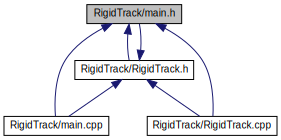
\includegraphics[width=350pt]{main_8h__dep__incl}
\end{center}
\end{figure}
\subsection*{Functions}
\begin{DoxyCompactItemize}
\item 
int \textbf{ start\+\_\+camera} ()
\begin{DoxyCompactList}\small\item\em start the loop that fetches frames, computes the position etc and sends it to other computers \end{DoxyCompactList}\item 
void \textbf{ start\+\_\+stop\+Camera} ()
\begin{DoxyCompactList}\small\item\em Start or stop the camera depending on if the camera is currently running or not. \end{DoxyCompactList}\item 
int \textbf{ set\+Zero} ()
\begin{DoxyCompactList}\small\item\em determine the initial position of the object that serves as reference point or as ground frame origin \end{DoxyCompactList}\item 
int \textbf{ calibrate\+\_\+camera} ()
\begin{DoxyCompactList}\small\item\em start the camera calibration routine that computes the camera matrix and distortion coefficients \end{DoxyCompactList}\item 
void \textbf{ load\+\_\+calibration} (int method)
\begin{DoxyCompactList}\small\item\em Load a previously saved camera calibration from a file. \end{DoxyCompactList}\item 
void \textbf{ test\+\_\+\+Algorithm} ()
\begin{DoxyCompactList}\small\item\em project some points from 3D to 2D and then check the accuracy of the algorithms \end{DoxyCompactList}\item 
void \textbf{ project\+Coordinate\+Frame} (Mat picture\+Frame)
\begin{DoxyCompactList}\small\item\em project a coordinate Co\+Sy with the rotation and translation of the object for visualization \end{DoxyCompactList}\item 
void \textbf{ set\+Up\+U\+DP} ()
\begin{DoxyCompactList}\small\item\em open the U\+DP ports for communication \end{DoxyCompactList}\item 
void \textbf{ set\+Heading\+Offset} (double d)
\begin{DoxyCompactList}\small\item\em Add a heading offset to the attitude for the case it is necessary. \end{DoxyCompactList}\item 
void \textbf{ send\+Data\+U\+DP} (cv\+::\+Vec3d \&Position, cv\+::\+Vec3d \&Euler)
\begin{DoxyCompactList}\small\item\em send the position and attitude over U\+DP to every receiver, the safety receiver is handled on its own in the start\+\_\+camera function \end{DoxyCompactList}\item 
void \textbf{ close\+U\+DP} ()
\begin{DoxyCompactList}\small\item\em close the U\+DP ports again to release network interfaces etc. \end{DoxyCompactList}\item 
void \textbf{ load\+Marker\+Config} (int method)
\begin{DoxyCompactList}\small\item\em load a marker configuration from file. This file has to be created by hand, use the standard marker configuration file as template \end{DoxyCompactList}\item 
void \textbf{ draw\+Position\+Text} (cv\+::\+Mat \&Picture, cv\+::\+Vec3d \&Position, cv\+::\+Vec3d \&Euler, double \textbf{ error})
\begin{DoxyCompactList}\small\item\em draw the position, attitude and reprojection error in the picture \end{DoxyCompactList}\item 
void \textbf{ load\+Camera\+Position} ()
\item 
int \textbf{ determine\+Exposure} ()
\begin{DoxyCompactList}\small\item\em get the optimal exposure for the camera. For that find the minimum and maximum exposure were the right number of markers are detected \end{DoxyCompactList}\item 
void \textbf{ determine\+Order} ()
\item 
int \textbf{ calibrate\+Ground} ()
\end{DoxyCompactItemize}
\subsection*{Variables}
\begin{DoxyCompactItemize}
\item 
int \textbf{ method\+P\+NP}
\begin{DoxyCompactList}\small\item\em set to true and the algorithm uses the last result as starting value \end{DoxyCompactList}\item 
bool \textbf{ safety\+Enable}
\item 
bool \textbf{ safety2\+Enable}
\begin{DoxyCompactList}\small\item\em is the safety feature enabled \end{DoxyCompactList}\item 
double \textbf{ safety\+Box\+Length}
\begin{DoxyCompactList}\small\item\em is the second receiver enabled \end{DoxyCompactList}\item 
int \textbf{ safety\+Angle}
\begin{DoxyCompactList}\small\item\em length of the safety area cube in meters \end{DoxyCompactList}\item 
Q\+Host\+Address \textbf{ I\+P\+Adress\+Object}
\begin{DoxyCompactList}\small\item\em socket for the communication with the rope winch \end{DoxyCompactList}\item 
Q\+Host\+Address \textbf{ I\+P\+Adress\+Safety}
\begin{DoxyCompactList}\small\item\em I\+Pv4 adress of the object wifi telemetry chip, can change to 192.\+168.\+4.\+x. This is where the position etc is sent to. \end{DoxyCompactList}\item 
Q\+Host\+Address \textbf{ I\+P\+Adress\+Safety2}
\begin{DoxyCompactList}\small\item\em I\+Pv4 adress of the circuit breaker, stays the same. \end{DoxyCompactList}\item 
int \textbf{ port\+Object}
\begin{DoxyCompactList}\small\item\em I\+Pv4 adress of the rope winch,. \end{DoxyCompactList}\item 
int \textbf{ port\+Safety}
\begin{DoxyCompactList}\small\item\em Port of the object. \end{DoxyCompactList}\item 
int \textbf{ port\+Safety2}
\begin{DoxyCompactList}\small\item\em Port of the safety switch. \end{DoxyCompactList}\item 
int \textbf{ invertZ}
\begin{DoxyCompactList}\small\item\em variable if tracking loop should be exited \end{DoxyCompactList}\item 
\textbf{ comm\+Object} \textbf{ comm\+Obj}
\end{DoxyCompactItemize}


\subsection{Function Documentation}
\mbox{\label{main_8h_a852329cf0943686665469e34f44a39bf}} 
\index{main.\+h@{main.\+h}!calibrate\+\_\+camera@{calibrate\+\_\+camera}}
\index{calibrate\+\_\+camera@{calibrate\+\_\+camera}!main.\+h@{main.\+h}}
\subsubsection{calibrate\+\_\+camera()}
{\footnotesize\ttfamily int calibrate\+\_\+camera (\begin{DoxyParamCaption}{ }\end{DoxyParamCaption})}



start the camera calibration routine that computes the camera matrix and distortion coefficients 

== Initialize Camera S\+DK ==--

== At this point the Camera S\+DK is actively looking for all connected cameras and will initialize == them on it\textquotesingle{}s own.

== Get a connected camera ================-\/---

== Determine camera resolution

== Set Video Mode ==--

== We set the camera to Segment Mode here. This mode is support by all of our products. == Depending on what device you have connected you might want to consider a different == video mode to achieve the best possible tracking quality. All devices that support a == mode that will achieve a better quality output with a mode other than Segment Mode are == listed here along with what mode you should use if you\textquotesingle{}re looking for the best head \subsection*{== tracking\+: }

== V100\+:R1/\+R2 Precision Mode == Track\+IR 5 Bit-\/\+Packed Precision Mode == V120 Precision Mode == T\+Bar Precision Mode \subsection*{== S250e Precision Mode }

== If you have questions about a new device that might be conspicuously missing here or == have any questions about head tracking, email support or participate in our forums.

== Start camera output ==--

== Camera Matrix creation ==--

== Ok, start main loop. This loop fetches and displays ===--- == camera frames. ===--- But first set some camera parameters

the user has to provide the size of one square in mm

== Fetch a new frame from the camera ===---

which is why we also set this constant to 8

later on, when we get the frame as usual\+:

== Lets have the Camera Library raster the camera\textquotesingle{}s == image into our texture.

imwrite(\char`\"{}test.\+jpg\char`\"{} + , mat\+Frame);

If done with success,

improve the found corners\textquotesingle{} coordinate accuracy for chessboard

== Release camera ==--

Save the obtained calibration coefficients in a file for later use


\begin{DoxyItemize}
\item File\+Storage\+::\+M\+E\+M\+O\+RY); 
\end{DoxyItemize}Here is the call graph for this function\+:\nopagebreak
\begin{figure}[H]
\begin{center}
\leavevmode
\includegraphics[width=345pt]{main_8h_a852329cf0943686665469e34f44a39bf_cgraph}
\end{center}
\end{figure}
Here is the caller graph for this function\+:\nopagebreak
\begin{figure}[H]
\begin{center}
\leavevmode
\includegraphics[width=343pt]{main_8h_a852329cf0943686665469e34f44a39bf_icgraph}
\end{center}
\end{figure}
\mbox{\label{main_8h_a7ad2e3cfb5056dbab2098e0dd3bd353f}} 
\index{main.\+h@{main.\+h}!calibrate\+Ground@{calibrate\+Ground}}
\index{calibrate\+Ground@{calibrate\+Ground}!main.\+h@{main.\+h}}
\subsubsection{calibrate\+Ground()}
{\footnotesize\ttfamily int calibrate\+Ground (\begin{DoxyParamCaption}{ }\end{DoxyParamCaption})}

Get the pose of the camera w.\+r.\+t the ground calibration frame. This frame sets the navigation frame for later results. The pose is averaged over 200 samples and then saved in the file reference\+Data.\+xml. This routine is basically the same as set\+Zero. initialize the variables with starting values

== Initialize Camera S\+DK ==--

== At this point the Camera S\+DK is actively looking for all connected cameras and will initialize == them on it\textquotesingle{}s own.

== Get a connected camera ================-\/---

== If no device connected, pop a message box and exit ==--

== Determine camera resolution to size application window ==-\/---

Set camera mode to precision mode, it directly provides marker coordinates

== Start camera output ==--

== Turn on some overlay text so it\textquotesingle{}s clear things are ===--- == working even if there is nothing in the camera\textquotesingle{}s view. ===--- Set some other parameters as well of the camera

sample some frames and calculate the position and attitude. then average those values and use that as zero position

== Fetch a new frame from the camera ===---

== Ok, we\textquotesingle{}ve received a new frame, lets do something == with it.

==for(int i=0; i$<$frame-\/$>$Object\+Count(); i++)

sort the 2d points with the correct indices as found in the preceeding order determination algorithm

Compute the pose from the 3\+D-\/2D corresponses

project the marker 3d points with the solution into the camera image Co\+Sy and calculate difference to true camera image

Iterative Method needs time to converge to solution

That are not the values of yaw, roll and pitch yet! Rodriguez has to be called first.

==-- one sample more \+:D

== Release camera ==--

Divide by the number of samples to get the mean of the reference position

euler\+Ref is here in Axis Angle notation

axis angle to rotation matrix ==-- Euler Angles, finally

rotation matrix to euler

Save the obtained calibration coefficients in a file for later use


\begin{DoxyItemize}
\item File\+Storage\+::\+M\+E\+M\+O\+RY); 
\end{DoxyItemize}Here is the call graph for this function\+:\nopagebreak
\begin{figure}[H]
\begin{center}
\leavevmode
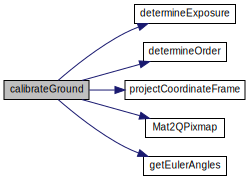
\includegraphics[width=350pt]{main_8h_a7ad2e3cfb5056dbab2098e0dd3bd353f_cgraph}
\end{center}
\end{figure}
Here is the caller graph for this function\+:\nopagebreak
\begin{figure}[H]
\begin{center}
\leavevmode
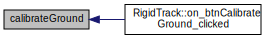
\includegraphics[width=337pt]{main_8h_a7ad2e3cfb5056dbab2098e0dd3bd353f_icgraph}
\end{center}
\end{figure}
\mbox{\label{main_8h_af2a8b7de0b15dc17198c147ba39e85f3}} 
\index{main.\+h@{main.\+h}!close\+U\+DP@{close\+U\+DP}}
\index{close\+U\+DP@{close\+U\+DP}!main.\+h@{main.\+h}}
\subsubsection{close\+U\+D\+P()}
{\footnotesize\ttfamily void close\+U\+DP (\begin{DoxyParamCaption}{ }\end{DoxyParamCaption})}



close the U\+DP ports again to release network interfaces etc. 

check if the socket is open and if yes close it Here is the call graph for this function\+:\nopagebreak
\begin{figure}[H]
\begin{center}
\leavevmode
\includegraphics[width=286pt]{main_8h_af2a8b7de0b15dc17198c147ba39e85f3_cgraph}
\end{center}
\end{figure}
Here is the caller graph for this function\+:\nopagebreak
\begin{figure}[H]
\begin{center}
\leavevmode
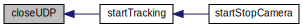
\includegraphics[width=350pt]{main_8h_af2a8b7de0b15dc17198c147ba39e85f3_icgraph}
\end{center}
\end{figure}
\mbox{\label{main_8h_a0416912fce6274568e80019b10ba294f}} 
\index{main.\+h@{main.\+h}!determine\+Exposure@{determine\+Exposure}}
\index{determine\+Exposure@{determine\+Exposure}!main.\+h@{main.\+h}}
\subsubsection{determine\+Exposure()}
{\footnotesize\ttfamily int determine\+Exposure (\begin{DoxyParamCaption}{ }\end{DoxyParamCaption})}



get the optimal exposure for the camera. For that find the minimum and maximum exposure were the right number of markers are detected 

== For Opti\+Track Ethernet cameras, it\textquotesingle{}s important to enable development mode if you == want to stop execution for an extended time while debugging without disconnecting == the Ethernet devices. Lets do that now\+:

== Initialize Camera S\+DK ==--

== At this point the Camera S\+DK is actively looking for all connected cameras and will initialize == them on it\textquotesingle{}s own.

== Get a connected camera ================-\/---

== If no device connected, pop a message box and exit ==--

== Determine camera resolution to size application window ==-\/---

set the camera mode to precision mode, it used greyscale imformation for marker property calculations

== Start camera output ==--

== Turn on some overlay text so it\textquotesingle{}s clear things are ===--- == working even if there is nothing in the camera\textquotesingle{}s view. ===---

set the camera exposure

set the camera infrared L\+ED intensity

set the camera framerate to 100 Hz

enable the filter that blocks visible light and only passes infrared light

enable high power mode of the leds

enable continuous L\+ED light

set threshold for marker detection

set exposure such that num markers are visible

Number of objects (markers) found in the current picture with the given exposure

exposure when objects detected the first time is number\+Markers

exposure when objects detected is first time number\+Markers+1

set the exposure to the smallest value possible

if the markers arent found after number\+Tries then there might be no markers at all in the real world

Determine minimum exposure, hence when are number\+Markers objects detected

get a new camera frame

frame received

how many objects are detected in the image

if the right amount if markers is found, exit while loop

not the right amount of markers was found so increase the exposure and try again

Now determine maximum exposure, hence when are number\+Markers+1 objects detected

if the markers arent found after number\+Tries then there might be no markers at all in the real world

how many objects are detected in the image

if the right amount if markers is found, exit while loop

not the right amount of markers was found so decrease the exposure and try again

set the exposure to the mean of min and max exposure determined

and now check if the correct amount of markers is detected with that new value

how many objects are detected in the image

are all markers and not more or less detected in the image

== Release camera ==--

all markers and not more or less are found Here is the call graph for this function\+:\nopagebreak
\begin{figure}[H]
\begin{center}
\leavevmode
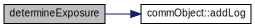
\includegraphics[width=327pt]{main_8h_a0416912fce6274568e80019b10ba294f_cgraph}
\end{center}
\end{figure}
Here is the caller graph for this function\+:\nopagebreak
\begin{figure}[H]
\begin{center}
\leavevmode
\includegraphics[width=350pt]{main_8h_a0416912fce6274568e80019b10ba294f_icgraph}
\end{center}
\end{figure}
\mbox{\label{main_8h_a11ff459289305229597defd39f510959}} 
\index{main.\+h@{main.\+h}!determine\+Order@{determine\+Order}}
\index{determine\+Order@{determine\+Order}!main.\+h@{main.\+h}}
\subsubsection{determine\+Order()}
{\footnotesize\ttfamily void determine\+Order (\begin{DoxyParamCaption}{ }\end{DoxyParamCaption})}

compute the order of the marker points in 2D so they are the same as in the 3D array. Hence marker 1 must be in first place for both, list\+\_\+points2d and list\+\_\+points3d determine the 3\+D-\/2D correspondences that are crucial for the PnP algorithm Try every possible correspondence and solve PnP Then project the 3D marker points into the 2D camera image and check the difference between projected points and points as seen by the camera the corresponce with the smallest difference is probably the correct one

the difference between true 2D points and projected points is super big

now try every possible permutation of correspondence

reset the starting values for solve\+PnP

sort the 2d points with the current permutation

Call solve P\+NP with P3P since its more robust and sufficient for start value determination

set the current difference of all point correspondences to zero

project the 3D points with the solve\+PnP solution onto 2D

now compute the absolute difference (error)

if the difference with the current permutation is smaller than the smallest value till now it is probably the more correct permutation

set the smallest value of difference to the current one

now safe the better permutation

try every permutation

now that the correct order is found assign it to the indices array Here is the caller graph for this function\+:\nopagebreak
\begin{figure}[H]
\begin{center}
\leavevmode
\includegraphics[width=350pt]{main_8h_a11ff459289305229597defd39f510959_icgraph}
\end{center}
\end{figure}
\mbox{\label{main_8h_af6430ad2592a955a3618549547dfc5be}} 
\index{main.\+h@{main.\+h}!draw\+Position\+Text@{draw\+Position\+Text}}
\index{draw\+Position\+Text@{draw\+Position\+Text}!main.\+h@{main.\+h}}
\subsubsection{draw\+Position\+Text()}
{\footnotesize\ttfamily void draw\+Position\+Text (\begin{DoxyParamCaption}\item[{cv\+::\+Mat \&}]{Picture,  }\item[{cv\+::\+Vec3d \&}]{Position,  }\item[{cv\+::\+Vec3d \&}]{Euler,  }\item[{double}]{error }\end{DoxyParamCaption})}



draw the position, attitude and reprojection error in the picture 

Here is the caller graph for this function\+:\nopagebreak
\begin{figure}[H]
\begin{center}
\leavevmode
\includegraphics[width=350pt]{main_8h_af6430ad2592a955a3618549547dfc5be_icgraph}
\end{center}
\end{figure}
\mbox{\label{main_8h_a44774828fee2764f3f3734bbd3f446e3}} 
\index{main.\+h@{main.\+h}!load\+\_\+calibration@{load\+\_\+calibration}}
\index{load\+\_\+calibration@{load\+\_\+calibration}!main.\+h@{main.\+h}}
\subsubsection{load\+\_\+calibration()}
{\footnotesize\ttfamily void load\+\_\+calibration (\begin{DoxyParamCaption}\item[{int}]{method }\end{DoxyParamCaption})}



Load a previously saved camera calibration from a file. 

Here is the call graph for this function\+:\nopagebreak
\begin{figure}[H]
\begin{center}
\leavevmode
\includegraphics[width=310pt]{main_8h_a44774828fee2764f3f3734bbd3f446e3_cgraph}
\end{center}
\end{figure}
Here is the caller graph for this function\+:\nopagebreak
\begin{figure}[H]
\begin{center}
\leavevmode
\includegraphics[width=350pt]{main_8h_a44774828fee2764f3f3734bbd3f446e3_icgraph}
\end{center}
\end{figure}
\mbox{\label{main_8h_af39fa6c3a36ad6bc24a327db7a9d73c2}} 
\index{main.\+h@{main.\+h}!load\+Camera\+Position@{load\+Camera\+Position}}
\index{load\+Camera\+Position@{load\+Camera\+Position}!main.\+h@{main.\+h}}
\subsubsection{load\+Camera\+Position()}
{\footnotesize\ttfamily void load\+Camera\+Position (\begin{DoxyParamCaption}{ }\end{DoxyParamCaption})}

load the rotation matrix from camera Co\+Sy to ground Co\+Sy It is determined during ground calibration and once the camera is mounted and fixed stays the same Open the reference\+Data.\+xml that contains the rotation from camera Co\+Sy to ground Co\+Sy Here is the call graph for this function\+:\nopagebreak
\begin{figure}[H]
\begin{center}
\leavevmode
\includegraphics[width=330pt]{main_8h_af39fa6c3a36ad6bc24a327db7a9d73c2_cgraph}
\end{center}
\end{figure}
Here is the caller graph for this function\+:\nopagebreak
\begin{figure}[H]
\begin{center}
\leavevmode
\includegraphics[width=350pt]{main_8h_af39fa6c3a36ad6bc24a327db7a9d73c2_icgraph}
\end{center}
\end{figure}
\mbox{\label{main_8h_a56c7f641859cb2b6b99b0947d03be800}} 
\index{main.\+h@{main.\+h}!load\+Marker\+Config@{load\+Marker\+Config}}
\index{load\+Marker\+Config@{load\+Marker\+Config}!main.\+h@{main.\+h}}
\subsubsection{load\+Marker\+Config()}
{\footnotesize\ttfamily void load\+Marker\+Config (\begin{DoxyParamCaption}\item[{int}]{method }\end{DoxyParamCaption})}



load a marker configuration from file. This file has to be created by hand, use the standard marker configuration file as template 

during start up of the programm load the standard marker configuration

open the standard marker configuration file

copy the values to the respective variables

inizialise vectors with correct length depending on the number of markers

save the marker locations in the points3d vector

if the load marker configuration button was clicked show a open file dialog

was cancel or abort clicked

if yes load the standard marker configuration

open the selected marker configuration file

copy the values to the respective variables

inizialise vectors with correct length depending on the number of markers

save the marker locations in the points3d vector

Print out the number of markers and their position to the G\+UI

check if P3P algorithm can be enabled, it needs exactly 4 marker points to work

if P3P is possible, let the user choose which algorithm he wants but keep iterative active

More (or less) marker than 4 loaded, P3P is not possible, hence user cant select P3P in G\+UI

now display the marker configuration in the camera view

Set the camera pose parallel to the marker coordinate system Here is the call graph for this function\+:\nopagebreak
\begin{figure}[H]
\begin{center}
\leavevmode
\includegraphics[width=344pt]{main_8h_a56c7f641859cb2b6b99b0947d03be800_cgraph}
\end{center}
\end{figure}
Here is the caller graph for this function\+:\nopagebreak
\begin{figure}[H]
\begin{center}
\leavevmode
\includegraphics[width=350pt]{main_8h_a56c7f641859cb2b6b99b0947d03be800_icgraph}
\end{center}
\end{figure}
\mbox{\label{main_8h_a2104a5d9d6b9f1e29bc4cd858c59882e}} 
\index{main.\+h@{main.\+h}!project\+Coordinate\+Frame@{project\+Coordinate\+Frame}}
\index{project\+Coordinate\+Frame@{project\+Coordinate\+Frame}!main.\+h@{main.\+h}}
\subsubsection{project\+Coordinate\+Frame()}
{\footnotesize\ttfamily void project\+Coordinate\+Frame (\begin{DoxyParamCaption}\item[{Mat}]{picture\+Frame }\end{DoxyParamCaption})}



project a coordinate Co\+Sy with the rotation and translation of the object for visualization 

z-\/axis

x-\/axis

y-\/axis Here is the caller graph for this function\+:\nopagebreak
\begin{figure}[H]
\begin{center}
\leavevmode
\includegraphics[width=350pt]{main_8h_a2104a5d9d6b9f1e29bc4cd858c59882e_icgraph}
\end{center}
\end{figure}
\mbox{\label{main_8h_a54b6b6db348b48d21e1265e22829c61f}} 
\index{main.\+h@{main.\+h}!send\+Data\+U\+DP@{send\+Data\+U\+DP}}
\index{send\+Data\+U\+DP@{send\+Data\+U\+DP}!main.\+h@{main.\+h}}
\subsubsection{send\+Data\+U\+D\+P()}
{\footnotesize\ttfamily void send\+Data\+U\+DP (\begin{DoxyParamCaption}\item[{cv\+::\+Vec3d \&}]{Position,  }\item[{cv\+::\+Vec3d \&}]{Euler }\end{DoxyParamCaption})}



send the position and attitude over U\+DP to every receiver, the safety receiver is handled on its own in the start\+\_\+camera function 

Roll Pitch Heading

if second receiver is activated send it also the tracking data Here is the caller graph for this function\+:\nopagebreak
\begin{figure}[H]
\begin{center}
\leavevmode
\includegraphics[width=350pt]{main_8h_a54b6b6db348b48d21e1265e22829c61f_icgraph}
\end{center}
\end{figure}
\mbox{\label{main_8h_ad19da4e648bbdc80d3123eb94711588e}} 
\index{main.\+h@{main.\+h}!set\+Heading\+Offset@{set\+Heading\+Offset}}
\index{set\+Heading\+Offset@{set\+Heading\+Offset}!main.\+h@{main.\+h}}
\subsubsection{set\+Heading\+Offset()}
{\footnotesize\ttfamily void set\+Heading\+Offset (\begin{DoxyParamCaption}\item[{double}]{d }\end{DoxyParamCaption})}



Add a heading offset to the attitude for the case it is necessary. 

Convert heading offset from degrees to rad

Calculate rotation about x axis

Calculate rotation about y axis

Calculate rotation about z axis

Combined rotation matrix Here is the caller graph for this function\+:\nopagebreak
\begin{figure}[H]
\begin{center}
\leavevmode
\includegraphics[width=350pt]{main_8h_ad19da4e648bbdc80d3123eb94711588e_icgraph}
\end{center}
\end{figure}
\mbox{\label{main_8h_ae624b0189bc5e32cbbb1f178b9f1a360}} 
\index{main.\+h@{main.\+h}!set\+Up\+U\+DP@{set\+Up\+U\+DP}}
\index{set\+Up\+U\+DP@{set\+Up\+U\+DP}!main.\+h@{main.\+h}}
\subsubsection{set\+Up\+U\+D\+P()}
{\footnotesize\ttfamily void set\+Up\+U\+DP (\begin{DoxyParamCaption}{ }\end{DoxyParamCaption})}



open the U\+DP ports for communication 

Initialise the Q\+Data\+Stream that stores the data to be send

Create U\+DP slots

if the safety feature is activated open the udp port

if the second receiver feature is activated open the udp port Here is the call graph for this function\+:\nopagebreak
\begin{figure}[H]
\begin{center}
\leavevmode
\includegraphics[width=288pt]{main_8h_ae624b0189bc5e32cbbb1f178b9f1a360_cgraph}
\end{center}
\end{figure}
Here is the caller graph for this function\+:\nopagebreak
\begin{figure}[H]
\begin{center}
\leavevmode
\includegraphics[width=350pt]{main_8h_ae624b0189bc5e32cbbb1f178b9f1a360_icgraph}
\end{center}
\end{figure}
\mbox{\label{main_8h_a7f3915653dcf5181fdc6e552ae8e6363}} 
\index{main.\+h@{main.\+h}!set\+Zero@{set\+Zero}}
\index{set\+Zero@{set\+Zero}!main.\+h@{main.\+h}}
\subsubsection{set\+Zero()}
{\footnotesize\ttfamily int set\+Zero (\begin{DoxyParamCaption}{ }\end{DoxyParamCaption})}



determine the initial position of the object that serves as reference point or as ground frame origin 

initialize the variables with starting values

== Initialize Camera S\+DK ==--

== At this point the Camera S\+DK is actively looking for all connected cameras and will initialize == them on it\textquotesingle{}s own.

== Get a connected camera ================-\/---

== If no device connected, pop a message box and exit ==--

== Determine camera resolution to size application window ==-\/---

Set camera mode to precision mode, it directly provides marker coordinates

== Start camera output ==--

== Turn on some overlay text so it\textquotesingle{}s clear things are ===--- == working even if there is nothing in the camera\textquotesingle{}s view. ===--- Set some other parameters as well of the camera

sample some frames and calculate the position and attitude. then average those values and use that as zero position

difference between the marker points as seen by the camera and the projected marker points with Rvec and Tvec

== Fetch a new frame from the camera ===---

== Ok, we\textquotesingle{}ve received a new frame, lets do something == with it.

==for(int i=0; i$<$frame-\/$>$Object\+Count(); i++)

sort the 2d points with the correct indices as found in the preceeding order determination algorithm

Compute the pose from the 3\+D-\/2D corresponses

project the marker 3d points with the solution into the camera image Co\+Sy and calculate difference to true camera image

Iterative Method needs time to converge to solution

That are not the values of yaw, roll and pitch yet! Rodriguez has to be called first.

==-- one sample more \+:D

== Release camera ==--

Divide by the number of samples to get the mean of the reference position

euler\+Ref is here in Axis Angle notation

axis angle to rotation matrix

==-- Euler Angles, finally

rotation matrix to euler

compute the difference between last obtained T\+Vec and the average Value When it is large the iterative method has not converged properly so it is advised to start the \doxyref{set\+Zero()}{p.}{main_8cpp_a7f3915653dcf5181fdc6e552ae8e6363} function once again Here is the call graph for this function\+:\nopagebreak
\begin{figure}[H]
\begin{center}
\leavevmode
\includegraphics[width=350pt]{main_8h_a7f3915653dcf5181fdc6e552ae8e6363_cgraph}
\end{center}
\end{figure}
Here is the caller graph for this function\+:\nopagebreak
\begin{figure}[H]
\begin{center}
\leavevmode
\includegraphics[width=281pt]{main_8h_a7f3915653dcf5181fdc6e552ae8e6363_icgraph}
\end{center}
\end{figure}
\mbox{\label{main_8h_a7d029857f86ebf6ac36e9a73508699ad}} 
\index{main.\+h@{main.\+h}!start\+\_\+camera@{start\+\_\+camera}}
\index{start\+\_\+camera@{start\+\_\+camera}!main.\+h@{main.\+h}}
\subsubsection{start\+\_\+camera()}
{\footnotesize\ttfamily int start\+\_\+camera (\begin{DoxyParamCaption}{ }\end{DoxyParamCaption})}



start the loop that fetches frames, computes the position etc and sends it to other computers 

The order of points, hence which entry in list\+\_\+points3d corresponds to which in list\+\_\+points2d is not calculated yet

Use the value of Rvec that was set in \doxyref{main()}{p.}{main_8cpp_a0ddf1224851353fc92bfbff6f499fa97} as starting value for the solve\+PnP algorithm

Use the value of Tvec that was set in \doxyref{main()}{p.}{main_8cpp_a0ddf1224851353fc92bfbff6f499fa97} as starting value for the solve\+PnP algorithm

Get the current date and time to name the log file

Concat the log file name as followed. The file is saved in the folder /logs in the Rigid Track installation folder

Convert the Q\+String to a standard string

Get the exposure where the right amount of markers is detected

For Opti\+Track Ethernet cameras, it\textquotesingle{}s important to enable development mode if you want to stop execution for an extended time while debugging without disconnecting the Ethernet devices. Lets do that now\+:

Initialize Camera S\+DK

At this point the Camera S\+DK is actively looking for all connected cameras and will initialize them on it\textquotesingle{}s own

Get a connected camera

If no camera can be found, inform user in message log and exit function

Determine camera resolution to size application window

Set the camera mode to precision mode, it used greyscale imformation for marker property calculations

Start camera output

Turn on some overlay text so it\textquotesingle{}s clear things are working even if there is nothing in the camera\textquotesingle{}s view

Set the camera exposure

Set the camera infrared L\+ED intensity

Set the camera framerate to 100 Hz

Enable the filter that blocks visible light and only passes infrared light

Enable high power mode of the L\+E\+Ds

Disable continuous L\+ED light

Set threshold for marker detection

Create a new matrix that stores the grayscale picture from the camera

Q\+Pixmap is the corresponding Qt class that saves images

Matrix that stores the colored picture, hence marker points, coordinate frame and reprojected points

Helper variable used to kick safety switch

Variables for the min and max values that are needed for sanity checks

Ff a marker is not visible or accuracy is bad increase this counter

Equals the quality of the tracking

Open sockets and ports for U\+DP communication

If the safety feature is enabled send the starting message

Send enable message, hence send a 9 and then a 1

Fetch a new frame from the camera

Get the timestamp of the first frame. This time is subtracted from every subseeding frame so the time starts at 0 in the logs

While no new frame is received loop

Get a new camera frame

There is actually a new frame

Get the time stamp for the first frame. It is subtracted for the following frames

Release the frame so the camera can continue

Exit the while loop

Now enter the main loop that processes each frame and computes the pose, sends it and logs stuff

Check if the user has not pressed \char`\"{}\+Stop Tracking\char`\"{} yet

Fetch a new frame from the camera

Did we got a new frame or does the camera still need more time

Increase by one, if everything is okay it is decreased at the end of the loop again

Only use this frame it the right number of markers is found in the picture

Get the marker points in 2D in the camera image frame and store them in the list\+\_\+points2d\+Unsorted vector The order of points that come from the camera corresponds to the Y coordinate

Was the order already determined? This is false for the first frame and from then on true

Now compute the order

Sort the 2d points with the correct indices as found in the preceeding order determination algorithm

point\+Order\+Indices was calculated in \doxyref{determine\+Order()}{p.}{main_8cpp_a11ff459289305229597defd39f510959}

The first time the 2\+D-\/3D corresspondence was determined with got\+Order was okay. But this order can change as the object moves and the marker objects appear in a different order in the frame-\/$>$Object() array. The solution is that\+: When a marker point (in the camera image, hence in 2D) was at a position then it wont move that much from one frame to the other. So for the new frame we take a marker object and check which marker was closest this point in the old image frame? This is probably the same (true) marker. And we do that for every other marker as well. When tracking is good and no frames are dropped because of missing markers this should work every frame.

The sum of point distances is set to something unrealistic large

Calculate N\+\_\+2 norm of unsorted points minus old points

If the norm is smaller than min\+Point\+Distance the correspondence is more likely to be correct

Update the array that saves the new point order

Now the new order is found, set the point order to the new value

Save the unsorted position of the marker points for the next loop

Compute the object pose from the 3\+D-\/2D corresponses

Project the marker 3d points with the solution into the camera image Co\+Sy and calculate difference to true camera image

Difference of true pose and found pose

Increase the frames\+Dropped variable if accuracy of tracking is too bad

Set number of subsequent frames dropped to zero because error is small enough and no marker was missing

Get the min and max values from T\+Vec for sanity check

Sanity check of values. negative z means the marker Co\+Sy is behind the camera, that\textquotesingle{}s not possible.

Release the frame so the camera can move on

Release the camera

Close all U\+DP connections so the programm can be closed later on and no resources are locked

Exit the function

Next step is the transformation from camera Co\+Sy to navigation Co\+Sy Compute the relative object position from the reference position to the current one given in the camera Co\+Sy\+: T\+\_\+\+C$^\wedge$\{NM\} = Tvec -\/ Tvec\+\_\+\{Ref\}

Transform the position from the camera Co\+Sy to the navigation Co\+Sy with I\+NS alligned heading and convert from [mm] to [m] T\+\_\+\+N$^\wedge$\{NM\} = M\+\_\+\{NC\}  T\+\_\+\+C$^\wedge$\{NM\}

Position is the result of the preceeding calculation

Invert Z if check box in G\+UI is activated, hence height above ground is considered

Realtive angle between reference orientation and current orientation

Convert axis angle respresentation to ordinary rotation matrix

The difference of the reference rotation and the current rotation R\+\_\+\{ NM \} = M\+\_\+\{ NC \}  R\+\_\+\{ CM \}

Euler Angles, finally

Get the euler angles from the rotation matrix

Add the heading offset to the heading angle

Compute the velocity with finite differences. Only use is the log file. It is done here because the more precise time stamp can be used

Time between the old frame and the current frame

Set the old frame time to the current one

Calculate the x velocity with finite differences

Calculate the y velocity with finite differences

Calculate the z velocity with finite differences

Set the old position to the current one for next frame velocity calcuation

Send position and Euler angles over Wi\+Fi with 100 Hz

Save the values in a log file, values are\+: Time sinc tracking started Position Euler Angles Velocity

Open the log file, the folder is Rigid\+Track\+Installation\+Folder/logs

Close the file to save values

Check if the position and euler angles are below the allowed value, if yes send O\+K\+AY signal (1), if not send shutdown signal (0) Absolute x, y and z position in navigation Co\+Sy must be smaller than the allowed distance

Absolute Euler angles must be smaller than allowed value. Heading is not considered

Send the O\+K\+AY signal to the desired computer every 5th time

Send the 1

reset the counter that is needed for decimation to every 5th time step

The euler angles of the object exceeded the allowed euler angles, send the shutdown signal (0)

Send the shutdown signal, a 0

Inform the user

The position of the object exceeded the allowed position, shut the object down

Send the shutdown signal, a 0

Inform the user

Inform the user if tracking system is disturbed (marker lost or so) or error was too big

Also send the shutdown signal

Send the shutdown signal, a 0

Inform the user

Rasterize the frame so it can be shown in the G\+UI

Convert the frame from greyscale as it comes from the camera to rgb color

Project (draw) the marker Co\+Sy origin into 2D and save it in the c\+Frame image

Project the marker points from 3D to the camera image frame (2d) with the computed pose

Draw a circle around the projected points so the result can be better compared to the real marker position In the resulting picture those are the red dots

Write the current position, attitude and error values as text in the frame

Send the new camera picture to the G\+UI and call the G\+UI processing routine

Update the picture in the G\+UI

Give Qt time to handle everything

Release the camera frame to fetch the new one

User choose to stop the tracking, clean things up

Close the U\+DP connections so resources are deallocated

Release camera Here is the call graph for this function\+:\nopagebreak
\begin{figure}[H]
\begin{center}
\leavevmode
\includegraphics[width=350pt]{main_8h_a7d029857f86ebf6ac36e9a73508699ad_cgraph}
\end{center}
\end{figure}
Here is the caller graph for this function\+:\nopagebreak
\begin{figure}[H]
\begin{center}
\leavevmode
\includegraphics[width=350pt]{main_8h_a7d029857f86ebf6ac36e9a73508699ad_icgraph}
\end{center}
\end{figure}
\mbox{\label{main_8h_a2daa058d8e8204f4e0c51cd8f7d0f962}} 
\index{main.\+h@{main.\+h}!start\+\_\+stop\+Camera@{start\+\_\+stop\+Camera}}
\index{start\+\_\+stop\+Camera@{start\+\_\+stop\+Camera}!main.\+h@{main.\+h}}
\subsubsection{start\+\_\+stop\+Camera()}
{\footnotesize\ttfamily void start\+\_\+stop\+Camera (\begin{DoxyParamCaption}{ }\end{DoxyParamCaption})}



Start or stop the camera depending on if the camera is currently running or not. 

tracking is not running so start it

tracking is currently running, set exit\+Request to true so the while loop in \doxyref{start\+\_\+camera()}{p.}{main_8cpp_a7d029857f86ebf6ac36e9a73508699ad} exits Here is the call graph for this function\+:\nopagebreak
\begin{figure}[H]
\begin{center}
\leavevmode
\includegraphics[width=350pt]{main_8h_a2daa058d8e8204f4e0c51cd8f7d0f962_cgraph}
\end{center}
\end{figure}
Here is the caller graph for this function\+:\nopagebreak
\begin{figure}[H]
\begin{center}
\leavevmode
\includegraphics[width=350pt]{main_8h_a2daa058d8e8204f4e0c51cd8f7d0f962_icgraph}
\end{center}
\end{figure}
\mbox{\label{main_8h_a49aae6cc1a72ace00943d9226b5070b3}} 
\index{main.\+h@{main.\+h}!test\+\_\+\+Algorithm@{test\+\_\+\+Algorithm}}
\index{test\+\_\+\+Algorithm@{test\+\_\+\+Algorithm}!main.\+h@{main.\+h}}
\subsubsection{test\+\_\+\+Algorithm()}
{\footnotesize\ttfamily void test\+\_\+\+Algorithm (\begin{DoxyParamCaption}{ }\end{DoxyParamCaption})}



project some points from 3D to 2D and then check the accuracy of the algorithms 

in mm

0 = iterative 1 = E\+P\+NP 2 = P3P 4 = U\+P\+NP //! not used

0 = iterative 1 = E\+P\+NP 2 = P3P 4 = U\+P\+NP //! not used

0 = iterative 1 = E\+P\+NP 2 = P3P 4 = U\+P\+NP //! not used

0 = iterative 1 = E\+P\+NP 2 = P3P 4 = U\+P\+NP //! not used Here is the call graph for this function\+:\nopagebreak
\begin{figure}[H]
\begin{center}
\leavevmode
\includegraphics[width=332pt]{main_8h_a49aae6cc1a72ace00943d9226b5070b3_cgraph}
\end{center}
\end{figure}
Here is the caller graph for this function\+:\nopagebreak
\begin{figure}[H]
\begin{center}
\leavevmode
\includegraphics[width=350pt]{main_8h_a49aae6cc1a72ace00943d9226b5070b3_icgraph}
\end{center}
\end{figure}


\subsection{Variable Documentation}
\mbox{\label{main_8h_af29e7fc07ae0979d5fb61b473241d33d}} 
\index{main.\+h@{main.\+h}!comm\+Obj@{comm\+Obj}}
\index{comm\+Obj@{comm\+Obj}!main.\+h@{main.\+h}}
\subsubsection{comm\+Obj}
{\footnotesize\ttfamily \textbf{ comm\+Object} comm\+Obj}

\mbox{\label{main_8h_a5cc3bd09f5801804b7ae65846e0b9824}} 
\index{main.\+h@{main.\+h}!invertZ@{invertZ}}
\index{invertZ@{invertZ}!main.\+h@{main.\+h}}
\subsubsection{invertZ}
{\footnotesize\ttfamily int invertZ}



variable if tracking loop should be exited 

\mbox{\label{main_8h_ab97ac0d82b1753d0eef37089be17e5e1}} 
\index{main.\+h@{main.\+h}!I\+P\+Adress\+Object@{I\+P\+Adress\+Object}}
\index{I\+P\+Adress\+Object@{I\+P\+Adress\+Object}!main.\+h@{main.\+h}}
\subsubsection{I\+P\+Adress\+Object}
{\footnotesize\ttfamily Q\+Host\+Address I\+P\+Adress\+Object}



socket for the communication with the rope winch 

\mbox{\label{main_8h_afefb1102a8a4a71b55d6f24f46404cc5}} 
\index{main.\+h@{main.\+h}!I\+P\+Adress\+Safety@{I\+P\+Adress\+Safety}}
\index{I\+P\+Adress\+Safety@{I\+P\+Adress\+Safety}!main.\+h@{main.\+h}}
\subsubsection{I\+P\+Adress\+Safety}
{\footnotesize\ttfamily Q\+Host\+Address I\+P\+Adress\+Safety}



I\+Pv4 adress of the object wifi telemetry chip, can change to 192.\+168.\+4.\+x. This is where the position etc is sent to. 

\mbox{\label{main_8h_a354806cf8cbface3575f2541d8fbcbda}} 
\index{main.\+h@{main.\+h}!I\+P\+Adress\+Safety2@{I\+P\+Adress\+Safety2}}
\index{I\+P\+Adress\+Safety2@{I\+P\+Adress\+Safety2}!main.\+h@{main.\+h}}
\subsubsection{I\+P\+Adress\+Safety2}
{\footnotesize\ttfamily Q\+Host\+Address I\+P\+Adress\+Safety2}



I\+Pv4 adress of the circuit breaker, stays the same. 

\mbox{\label{main_8h_ab5e634b66221f494504aea1557af5df9}} 
\index{main.\+h@{main.\+h}!method\+P\+NP@{method\+P\+NP}}
\index{method\+P\+NP@{method\+P\+NP}!main.\+h@{main.\+h}}
\subsubsection{method\+P\+NP}
{\footnotesize\ttfamily int method\+P\+NP}



set to true and the algorithm uses the last result as starting value 

\mbox{\label{main_8h_a9a00043c93a3362969c1c1fcd3a70fea}} 
\index{main.\+h@{main.\+h}!port\+Object@{port\+Object}}
\index{port\+Object@{port\+Object}!main.\+h@{main.\+h}}
\subsubsection{port\+Object}
{\footnotesize\ttfamily int port\+Object}



I\+Pv4 adress of the rope winch,. 

\mbox{\label{main_8h_a137bc8cc9d53ad9b176c988a99bc7142}} 
\index{main.\+h@{main.\+h}!port\+Safety@{port\+Safety}}
\index{port\+Safety@{port\+Safety}!main.\+h@{main.\+h}}
\subsubsection{port\+Safety}
{\footnotesize\ttfamily int port\+Safety}



Port of the object. 

\mbox{\label{main_8h_a2601be9c226be24c71ec8282f632e723}} 
\index{main.\+h@{main.\+h}!port\+Safety2@{port\+Safety2}}
\index{port\+Safety2@{port\+Safety2}!main.\+h@{main.\+h}}
\subsubsection{port\+Safety2}
{\footnotesize\ttfamily int port\+Safety2}



Port of the safety switch. 

\mbox{\label{main_8h_a436fb814ccc3f02617dade4dc6511143}} 
\index{main.\+h@{main.\+h}!safety2\+Enable@{safety2\+Enable}}
\index{safety2\+Enable@{safety2\+Enable}!main.\+h@{main.\+h}}
\subsubsection{safety2\+Enable}
{\footnotesize\ttfamily bool safety2\+Enable}



is the safety feature enabled 

\mbox{\label{main_8h_ae65386c3310ab826e84fba757296de9a}} 
\index{main.\+h@{main.\+h}!safety\+Angle@{safety\+Angle}}
\index{safety\+Angle@{safety\+Angle}!main.\+h@{main.\+h}}
\subsubsection{safety\+Angle}
{\footnotesize\ttfamily int safety\+Angle}



length of the safety area cube in meters 

\mbox{\label{main_8h_a2c1b807fcb2de5a6759bd60ccae6dd7e}} 
\index{main.\+h@{main.\+h}!safety\+Box\+Length@{safety\+Box\+Length}}
\index{safety\+Box\+Length@{safety\+Box\+Length}!main.\+h@{main.\+h}}
\subsubsection{safety\+Box\+Length}
{\footnotesize\ttfamily double safety\+Box\+Length}



is the second receiver enabled 

\mbox{\label{main_8h_aa6266eedab8b3c011be53baffbfc42ab}} 
\index{main.\+h@{main.\+h}!safety\+Enable@{safety\+Enable}}
\index{safety\+Enable@{safety\+Enable}!main.\+h@{main.\+h}}
\subsubsection{safety\+Enable}
{\footnotesize\ttfamily bool safety\+Enable}


\hypertarget{_rigid_track_8cpp}{}\section{Rigid\+Track/\+Rigid\+Track.cpp File Reference}
\label{_rigid_track_8cpp}\index{Rigid\+Track/\+Rigid\+Track.\+cpp@{Rigid\+Track/\+Rigid\+Track.\+cpp}}


Rigid Track G\+UI source that contains functions for G\+UI events.  


{\ttfamily \#include \char`\"{}Rigid\+Track.\+h\char`\"{}}\newline
{\ttfamily \#include $<$Q\+Process$>$}\newline
{\ttfamily \#include $<$Qdesktop\+Services$>$}\newline
{\ttfamily \#include $<$Q\+Dir$>$}\newline
{\ttfamily \#include $<$Q\+Message\+Box$>$}\newline
{\ttfamily \#include $<$Q\+Url$>$}\newline
{\ttfamily \#include \char`\"{}main.\+h\char`\"{}}\newline
{\ttfamily \#include \char`\"{}communication.\+h\char`\"{}}\newline
{\ttfamily \#include $<$exception$>$}\newline
Include dependency graph for Rigid\+Track.\+cpp\+:
\nopagebreak
\begin{figure}[H]
\begin{center}
\leavevmode
\includegraphics[width=350pt]{_rigid_track_8cpp__incl}
\end{center}
\end{figure}


\subsection{Detailed Description}
Rigid Track G\+UI source that contains functions for G\+UI events. 

\begin{DoxyAuthor}{Author}
Florian J.\+T. Wachter 
\end{DoxyAuthor}
\begin{DoxyVersion}{Version}
1.\+0 
\end{DoxyVersion}
\begin{DoxyDate}{Date}
April, 8th 2017 
\end{DoxyDate}

\hypertarget{_rigid_track_8h}{}\section{Rigid\+Track/\+Rigid\+Track.h File Reference}
\label{_rigid_track_8h}\index{Rigid\+Track/\+Rigid\+Track.\+h@{Rigid\+Track/\+Rigid\+Track.\+h}}
{\ttfamily \#include $<$Qt\+Widgets/\+Q\+Main\+Window$>$}\newline
{\ttfamily \#include \char`\"{}ui\+\_\+\+Rigid\+Track.\+h\char`\"{}}\newline
{\ttfamily \#include $<$qpixmap.\+h$>$}\newline
{\ttfamily \#include \char`\"{}main.\+h\char`\"{}}\newline
{\ttfamily \#include \char`\"{}communication.\+h\char`\"{}}\newline
Include dependency graph for Rigid\+Track.\+h\+:\nopagebreak
\begin{figure}[H]
\begin{center}
\leavevmode
\includegraphics[width=350pt]{_rigid_track_8h__incl}
\end{center}
\end{figure}
This graph shows which files directly or indirectly include this file\+:\nopagebreak
\begin{figure}[H]
\begin{center}
\leavevmode
\includegraphics[width=350pt]{_rigid_track_8h__dep__incl}
\end{center}
\end{figure}
\subsection*{Classes}
\begin{DoxyCompactItemize}
\item 
class \hyperlink{class_rigid_track}{Rigid\+Track}
\end{DoxyCompactItemize}

%--- End generated contents ---

% Index
\backmatter
\newpage
\phantomsection
\clearemptydoublepage
\addcontentsline{toc}{chapter}{Index}
\printindex

\end{document}